%%%%%%%% ICML 2020 EXAMPLE LATEX SUBMISSION FILE %%%%%%%%%%%%%%%%%

\documentclass{article}
\usepackage{times}
\usepackage{epsfig}
\usepackage{graphicx}
\usepackage{amsmath}
\usepackage{amssymb}
\usepackage{times}
\usepackage{epsfig}
\usepackage{graphicx}
\usepackage{amsmath}
\usepackage{amssymb}
% Include other packages here, before hyperref.
\usepackage{xcolor}
\usepackage[ruled,vlined,onelanguage]{algorithm2e}
\usepackage{setspace}
\usepackage{collcell}
\usepackage{xr}
\usepackage{natbib}
\usepackage{multirow}
\usepackage{subcaption}
\usepackage{mathtools}
\usepackage{colortbl,dcolumn}
\usepackage{algorithm2e}
\usepackage{standalone}

% Include other packages here, before hyperref.

% If you comment hyperref and then uncomment it, you should delete
% egpaper.aux before re-running latex.  (Or just hit 'q' on the first latex
% run, let it finish, and you should be clear).
\usepackage[pagebackref=true,breaklinks=true,letterpaper=true,colorlinks,bookmarks=false]{hyperref}

% \cvprfinalcopy % *** Uncomment this line for the final submission

\def\cvprPaperID{****} % *** Enter the CVPR Paper ID here
\def\httilde{\mbox{\tt\raisebox{-.5ex}{\symbol{126}}}}

\newcommand{\todo}[1]{{\color{blue}TODO #1}}
\newcommand{\toref}[1]{{\color{red}REF #1 }}
\newcommand{\registered}{\textsuperscript{\tiny\textregistered}}
%\newcommand{\etal}{\textit{et al.}}
\renewcommand{\eqref}[1]{\hyperref[#1]{Eq.\ \ref*{#1}}}
\newcommand{\figref}[1]{\hyperref[#1]{Fig.\ \ref*{#1}}}
\newcommand{\tabref}[1]{\hyperref[#1]{Table\ \ref*{#1}}}
\newcommand{\secref}[1]{\hyperref[#1]{Section\ \ref*{#1}}}
\newcommand{\algoref}[1]{\hyperref[#1]{Algorithm\ \ref*{#1}}}
\newcolumntype{C}[1]{>{\centering}m{#1}}
\newcommand{\N}{{\cal N}}
\newcommand{\std}[1]{ \normalfont \color{darkgray}\footnotesize{$\pm$#1} }

% SYMBOL
\newcommand{\E}{{\mathbb E}}
\newcommand{\Q}{{\mathbb Q}}

\hypersetup{
    colorlinks=true,
    linkcolor=blue,
    filecolor=magenta,      
    urlcolor=blue,
}

\urlstyle{same}

% Recommended, but optional, packages for figures and better typesetting:
\usepackage{microtype}
\usepackage{booktabs} % for professional tables
\setlength{\abovedisplayskip}{-2pt}
\setlength{\belowdisplayskip}{-2pt}

% hyperref makes hyperlinks in the resulting PDF.
% If your build breaks (sometimes temporarily if a hyperlink spans a page)
% please comment out the following usepackage line and replace
% \usepackage{icml2020} with \usepackage[nohyperref]{icml2020} above.
\usepackage{hyperref}

% Attempt to make hyperref and algorithmic work together better:
\newcommand{\theHalgorithm}{\arabic{algorithm}}

% Use the following line for the initial blind version submitted for review:
%\usepackage{icml2020}

% If accepted, instead use the following line for the camera-ready submission:
\usepackage[accepted]{icml2020}

% The \icmltitle you define below is probably too long as a header.
% Therefore, a short form for the running title is supplied here:
\icmltitlerunning{Bayesian active learning for production}
\begin{document}

\twocolumn[
\icmltitle{Bayesian active learning for production, a systematic study and a reusable library}

% It is OKAY to include author information, even for blind
% submissions: the style file will automatically remove it for you
% unless you've provided the [accepted] option to the icml2020
% package.

% List of affiliations: The first argument should be a (short)
% identifier you will use later to specify author affiliations
% Academic affiliations should list Department, University, City, Region, Country
% Industry affiliations should list Company, City, Region, Country

% You can specify symbols, otherwise they are numbered in order.
% Ideally, you should not use this facility. Affiliations will be numbered
% in order of appearance and this is the preferred way.
\icmlsetsymbol{equal}{*}

\begin{icmlauthorlist}
\icmlauthor{Parmida Atighehchian}{equal,eai}
\icmlauthor{Fr\'ed\'eric Branchaud-Charron}{equal,eai}
\icmlauthor{Alexandre Lacoste}{eai}
\end{icmlauthorlist}

\icmlaffiliation{eai}{Element AI, Montr\'eal, Canada}

\icmlcorrespondingauthor{Fr\'ed\'eric Branchaud-Charron}{frederic.branchaud-charron@elementai.com}

% You may provide any keywords that you
% find helpful for describing your paper; these are used to populate
% the "keywords" metadata in the PDF but will not be shown in the document
\icmlkeywords{Machine Learning, Active Learning, Uncertainty Estimation}

\vskip 0.3in
]

% this must go after the closing bracket ] following \twocolumn[ ...

% This command actually creates the footnote in the first column
% listing the affiliations and the copyright notice.
% The command takes one argument, which is text to display at the start of the footnote.
% The \icmlEqualContribution command is standard text for equal contribution.
% Remove it (just {}) if you do not need this facility.

%\printAffiliationsAndNotice{}  % leave blank if no need to mention equal contribution
\printAffiliationsAndNotice{\icmlEqualContribution} % otherwise use the standard text.

\begin{figure}
    \centering
    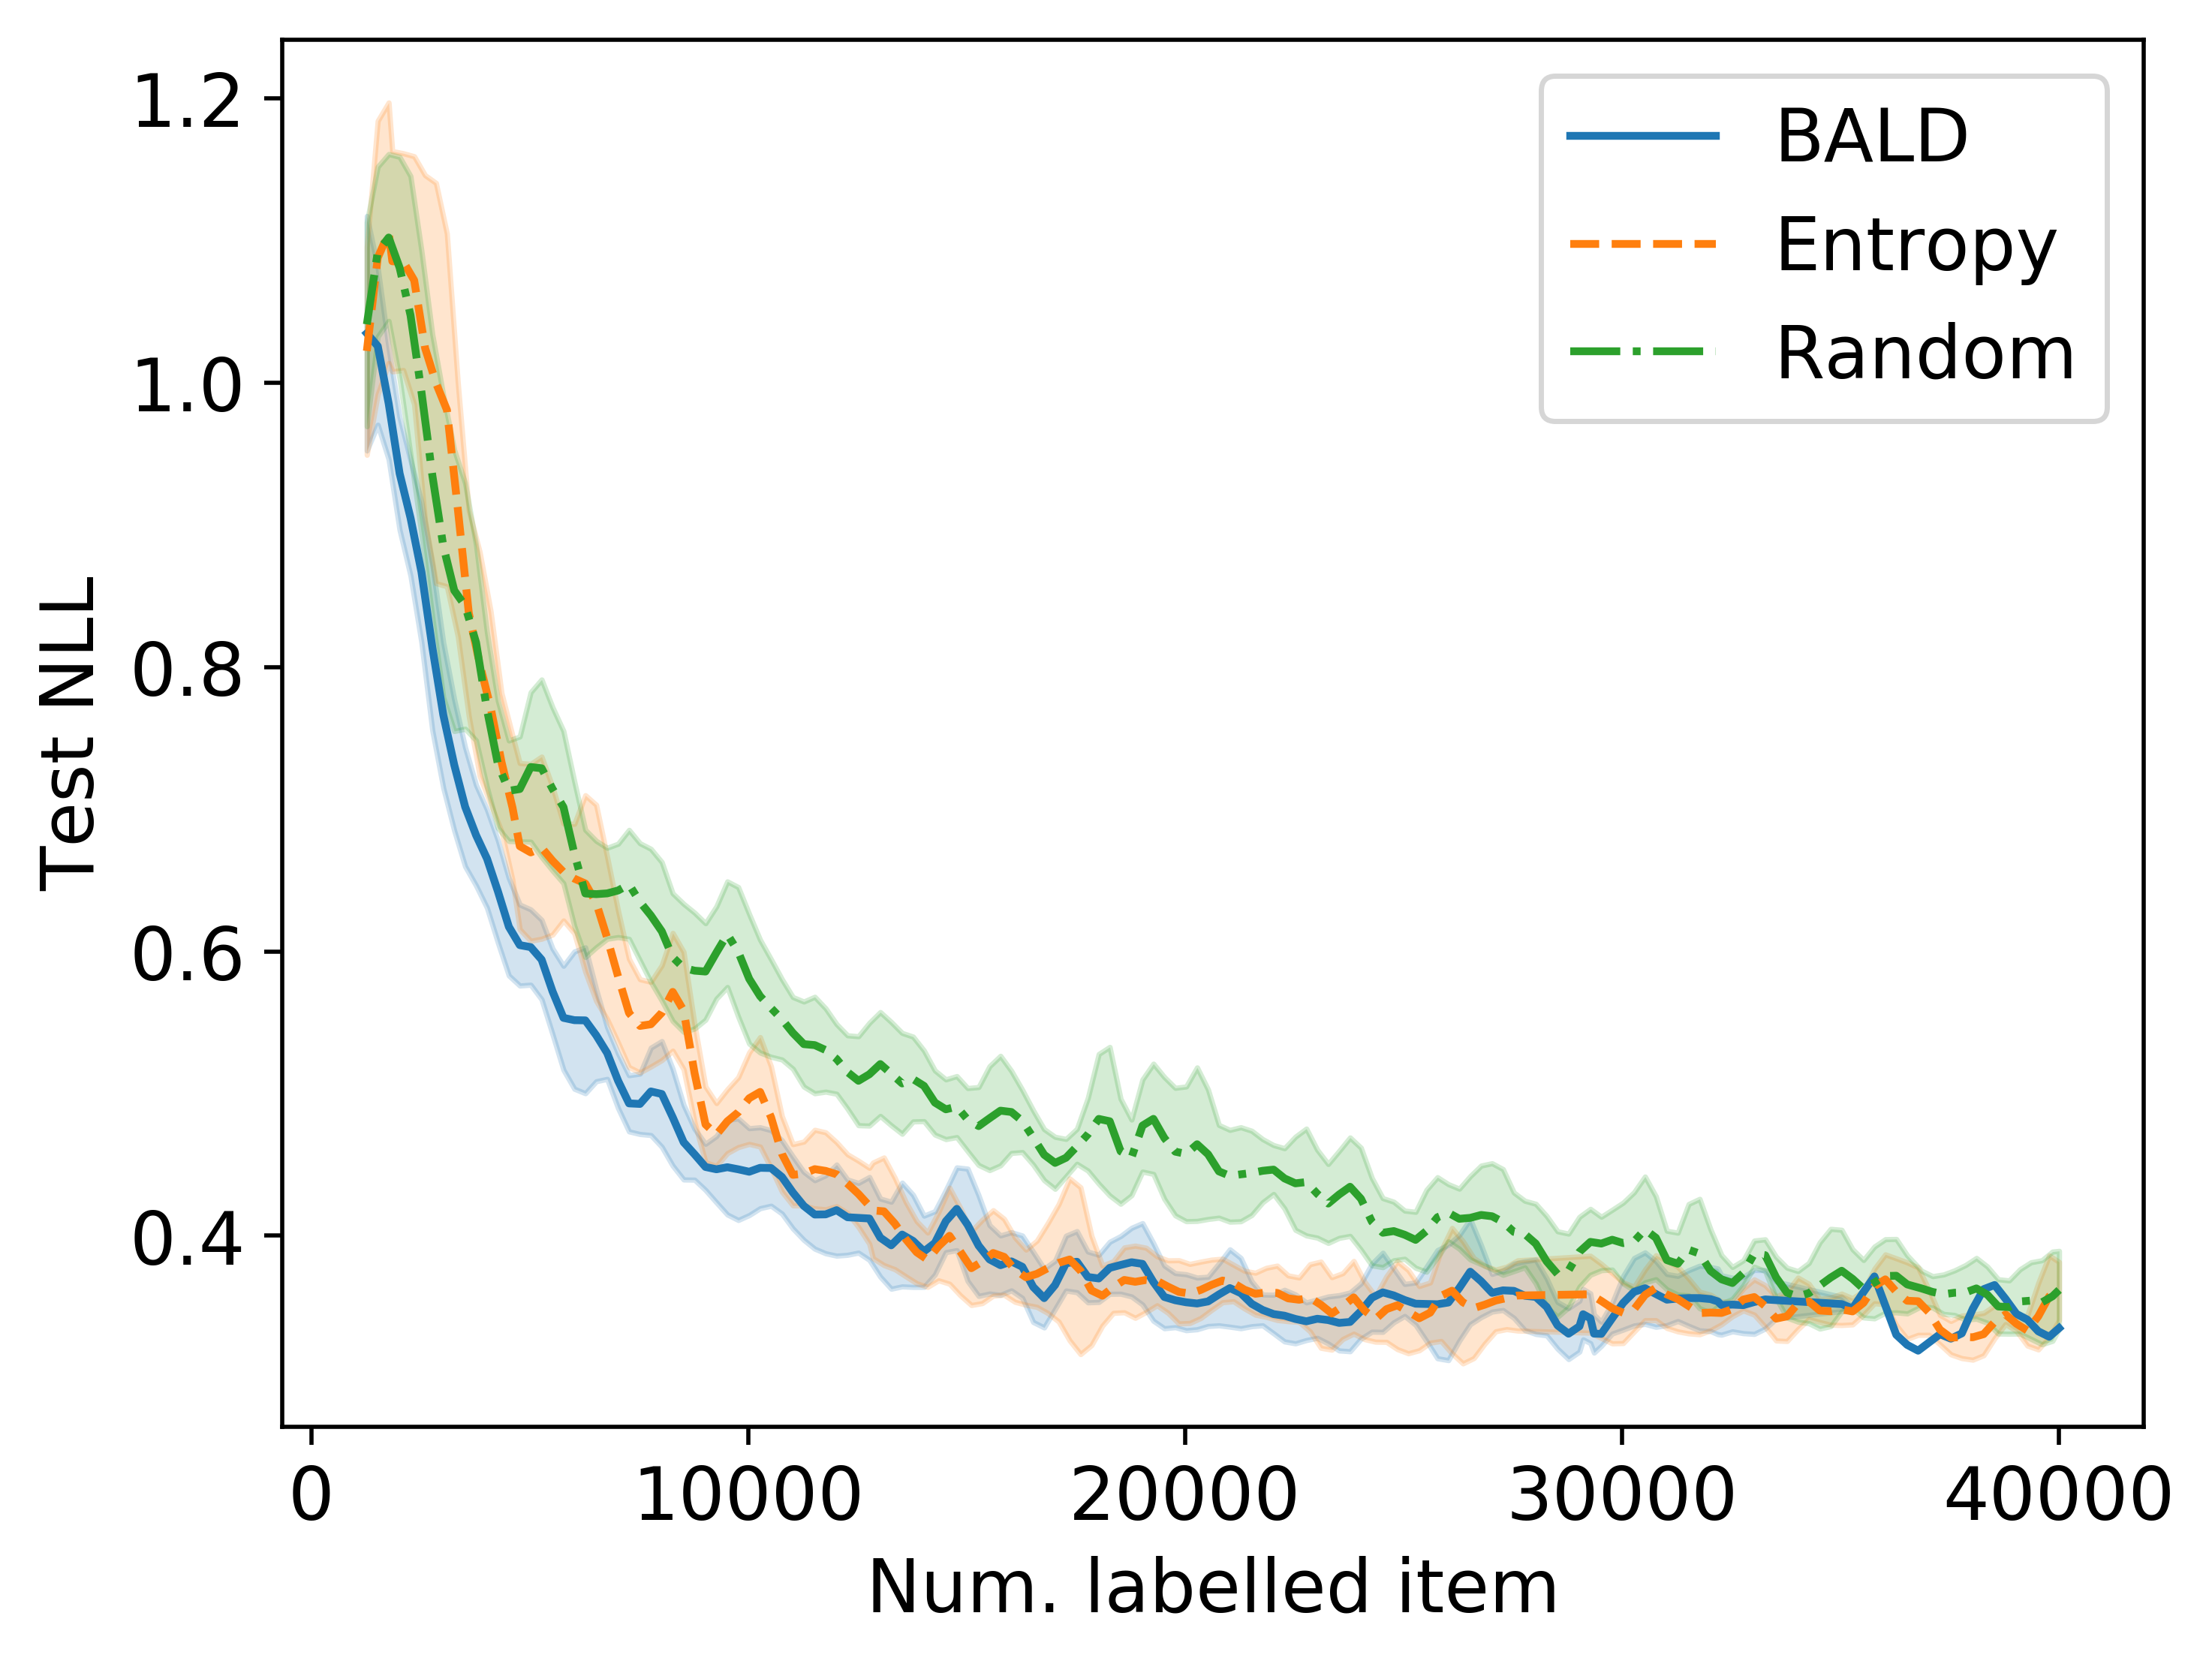
\includegraphics[width=0.4\textwidth]{fig/standard.png}
    \caption{Baselines results on CIFAR10 using MC-Dropout and VGG-16. On an academic dataset, both active learning techniques are competitive.}
    \label{fig:standard}
\end{figure}

\begin{abstract}
\vspace{-0.60cm}
   Active learning is able to reduce the amount of labelling effort by using a machine learning model to query the user for specific inputs.
   While there are many papers on new active learning techniques, these techniques rarely satisfy the constraints of a real-world project. In this paper, we analyse the main drawbacks of current active learning techniques and we present approaches to alleviate them. We do a systematic study on the effects of the most common issues of real-world datasets on the deep active learning process: model convergence, annotation error, and dataset imbalance. We derive two techniques that can speed up the active learning loop such as partial uncertainty sampling and larger query size. Finally, we present our open-source Bayesian active learning library, BaaL.
\end{abstract}

%%%%%%%%% BODY TEXT

%%%%%%%%%%%%%%%%%%%%%%%%%%%
%% See https://docs.google.com/document/d/148Rkq9R44TIT4QdDR8jsHhQ3zBIPdbVbrjEFkod4hV8/edit?usp=sharing
%%%%%%%%%%%%%%%%%%%%%%%%%%%%
\section{Introduction}
The amount of data readily available for machine learning has exploded in recent years. 
However, for data to be used for deep learning models, labelling is often a required step. 
A common problem when labelling new datasets is the required human effort to perform the annotation. In particular, tasks that require particular domain knowledge such as medical imaging, are expensive to annotate. To solve this, active learning (AL) has been proposed to only label the core set of observations useful for training.

While the active learning field includes many approaches \citep{kirsch2019batchbald, tsymbalov2019deeper, beluch2018power, maddox2019simple}, these methods are often not scalable to large datasets or too slow to be used in a more realistic environment e.g. in a production setup. In particular, active learning applied to images or text requires the usage of deep learning models which are slow to train and themselves require a noticeable huge amount of data to be effective \citep{imagenet_cvpr09, abu2016youtube}.

Furthermore, deep learning models require carefully tuned hyperparameters to be effective. In a research environment, one can fine-tune and perform hyperparameter search to find the optimal combination that gives the biggest reduction in labelling  effort. In a real-world setting, the hyperparameters are set at the beginning with no guarantee for the outcome.

Finally, in a real-world setup, the data is often not cleaned nor balanced. In particular, studies have shown that humans are far from perfect when labelling and the problem is even worse when using crowd-sourcing \citep{ipeirotis2010quality, allahbakhsh2013quality}.

Our contributions are three-fold. We perform a systematic study on the effect of the most common pathologies found in real-world datasets on active learning. Second, we propose several techniques that make active learning suitable for production. Finally, we present a case study of using active learning on a real-world dataset. 

In addition, we present our freely available Bayesian active learning library, BaaL\footnote{\url{https://github.com/ElementAI/baal}} which provides all the necessary set up and tools for active learning experiments at any scale.

\section{Problem setting}

We consider the problem of supervised learning where we observe a dataset made of $n$ pairs $D_L= \{(x_i, y_i)\}_i^{N}$ and our goal is to estimate a prediction function $p(y\mid x)$. In addition, we have $N'$ observations without label $D_U = \{x_i\}_i^{N'}$. More specifically, we consider the problem of active learning where the algorithm is summarized in \algoref{algo:al}.

\begin{algorithm}
 \KwData{$D = \{x_0, \ldots, x_n\}$}
 \KwResult{$D_L = \{(x_0, y_0), \ldots\}$}
 ~~$D_L \leftarrow$ Label randomly B points\;\\
 $D_U \leftarrow D \setminus D_L$ \;\\
\While{labelling budget is available}{
  Train model to convergence on $D_L$\;\\
  Compute uncertainty $U(x), \text{for all } x \in D_U$\;\\
  Label top-\textit{k} most uncertain samples\;
 }
 \caption{\textbf{Active learning process.} For batch active learning, the algorithm train a model on $D_L$ before estimating the uncertainty on the pool $D_U$, the most uncertain samples are labelled by a human before restarting the loop.}
 \label{algo:al}
\end{algorithm}

%-------------------------------------------------------------------------
\section{Background}\label{background}
%The goal of active learning is to reduce the labelling effort without giving up on model performance. Deep Learning models are powerful solutions given a good representation of the domain \citep{krizhevsky2012imagenet, ioffe2015batch}. Unfortunately, acquiring and labelling  data is a tedious, time-consuming and expensive task. Reducing the number of samples we need to label is key to make deep learning more affordable.
% ICML CUT In the past years, there have been different attempts of adjusting active learning for deep learning models. The most complete literature for active learning is concentrated on
Active learning has received a lot of attention in the past years, specifically on classification tasks \citep{gal2017deep}. However, some work has been done on segmentation \citep{kendall2017uncertainties}, localization \citep{miller2019evaluating}, natural language processing \citep{siddhant2018deep}, and time series \citep{peng2017acts}. In this paper, we focus our attention on image classification. %There are several challenges involved in changing the training procedure of a model to active training. 

\paragraph{Bayesian active Learning}
Current state-of-the-art techniques used in active learning relies on uncertainty estimation to perform queries~\citep{gal2017deep}.
%\todo{No evidence, needs at least a ref: For once, the more complicated the task, the harder to estimate the model uncertainty and hence, it is more challenging to achieve the state of the art model accuracy/precision with active learning.} 
%The  active learning procedure is time-consuming due to the need to retrain the model between queries. In a perfect scenario, one would imagine to have an active training framework in which the annotator could get new queries to be labelled as soon as possible, i.e. the model should be fast enough to compute the uncertainty between each sample labelled. 
A common issue highlighted in \citet{tsymbalov2019deeper, kirsch2019batchbald} is the need to retrain the model and recompute the uncertainties as often as possible. Otherwise, the next samples to be selected may be too similar to previously annotated samples. This is problematic due to the long training time of deep-learning models as well as the expensive task of uncertainty estimation.
\citet{tsymbalov2019deeper, houlsby2011bayesian} and \citet{Wilson2015DeepKL} proposed solutions to this issue, are memory expensive and time-consuming when used on large input size or large datasets.
In reality, due to the large cost of inference and retraining for large scale datasets, it is not feasible to recompute the uncertainties in a timely fashion. In consequence, multiple samples are annotated between retraining. We call this framework batch active learning.

%FRED: This needs to be moved
% The idea behind bayesian active learning is simple, the model is able to to actively “query” example(s) to be labelled. By doing that, we hope to label only the most effective samples for training the model instead of random selection. 
%CUT ICML There are, at a high level, two types of strategies for choosing data points for labelling . One is to sample data points you hope will be most representative of your dataset as a whole, in order for any model you train to quickly learn features that represent fundamental variation in the data. The other is to choose data points that will maximize the information gain from a model trained in parallel.
%CUT ICML Sampling data points at random is a naive example of the first strategy. It would sample from the data distribution which contains uninformative samples. However, there are ways to improve on this, for example by clustering the data and using this cluster structure to sample a diverse representative set of observation. \citet{sener2017active} are proposed as a way to extract a subset representative of the overall distribution of the dataset. In this paper, we will focus on the second strategy.
Machine leanings algorithms can suffer from two types of uncertainties \citep{kendall2017uncertainties}:

1) \emph{Aleatoric Uncertainty}, the uncertainty intrinsic to the data, which cannot be explained with more samples. This is due to e.g.: errors during labelling, occlusion, poor data acquisition ,or when two classes are highly confused. 

2) \emph{Epistemic Uncertainty}, the uncertainty about the underlying model. Obtaining more samples will provide more information about the underlying model and reduce the amount of epistemic uncertainty. Crucially, some samples are more informative than others. 

\paragraph{Uncertainty estimations} 
Computing the uncertainty of deep neural networks is crucial to many applications from medical imaging to loan application. Unfortunately, deep neural networks are often overconfident as they are not designed to provide calibrated predictions \citep{scalia2019evaluating,gal2016uncertainty}. Hence, researchers proposed new methods to get a trustful estimation of the epistemic uncertainty such as MC-Dropout \citep{gal2016dropout}, Bayesian neural networks \citep{blundell2015weight} or Ensembles. More recently, \citet{wilson2020bayesian} proposed to combine variational inference and ensembles. While this approach is state-of-the-art, it is far too computationally expensive to be used in the industry.

%In this paper, we will focus on MC-Dropout because it can be used with most common architectures and has a non-prohibitive inference time when optimally implemented.

In this paper, we will use MC-Dropout \citep{gal2016dropout}. In this technique proposes the Dropout layers are kept activated at test time to sample from the posterior distribution. Hence, this method can be used on any architecture that uses Dropout which makes it usable on a wide range of applications.

% Should we say that BNN estimates both aleactoric and epistemic while MCDropout + BALD just estimate epistemic (Gal et al.)

\paragraph{Acquisition functions}
Many heuristics have been proposed to extract the uncertainty value from the stochastic prediction sampling. We define  Monte-Carlo sampling from the posterior distribution $p(w\mid D)$ as:
\begin{equation*}
    p_t(y \mid x) = p(y \mid x, w_t), t \in \{1 \ldots T\}, w_t \sim p(w\mid D)
\end{equation*}

where $T$ is the number of Monte-Carlo samples. %For example, a classification task with $C$ classes, $p$ contains a matrix $C\times T$.
We compute the Bayesian model average, $\hat p(y \mid x) = \frac{1}{T} \sum_t^T p_t(y \mid x)$. When highly uncertain, $\hat p(y \mid x)$ will be close to a uniform distribution. A naive approach to estimate the uncertainty is to compute the entropy of this distribution.

% \begin{align*}
%     U(x) =& \sum_c \hat p(y = c \mid x) * \log(\hat p(y = c \mid x)).
% \end{align*}

% By assuming a Gaussian prior over the weights, we can compute 
% \begin{equation*}
%     U(X) = \E_c[Var(p(y=c \mid x))]
% \end{equation*}
% the expected variance of the model.

A more sophisticated approach is BALD~\citep{houlsby2011bayesian}, which estimates the epistemic uncertainty by computing the mutual information between the model posterior distribution and the prediction:
\begin{equation*}
    I(y, w \mid x, D_L) = H[y \mid x, D_L] - \E_{p(w \mid D_L)}(H[y \mid x, w]).
\end{equation*}


BALD compares the entropy of the mean estimator to the entropies of all estimators. The result is high when there are high disagreements between predictions, which addresses the overconfidence issue in deep learning models.

% We can combine this network with MC-Dropout such that the BALD uncertainty can be computed with:

% \begin{align*}
%     U(x) &= H[y \mid x, D_L] - \E_{p(w \mid D_L)}(H[y \mid x, w]) \\
%     &= H[y \mid x, D_L] - \frac{1}{T} \sum_t^T \sum_c^C f_c(x) \log f_c(x) \\
%     &= \hat f(x) \log \hat f(x) - \frac{1}{T} \sum_t^T \sum_c^C f_c(x) \log f_c(x). 
% \end{align*}

\section{Experiments}

In this paper, we want to demonstrate the usability of active learning in a real-world scenario. First, we analyze the effect of common pathologies in deep learning on active learning. Secondly, a common issue in active learning is the time required between steps in the active learning loop. As stated by \citet{kirsch2019batchbald}, retraining as soon as possible is crucial to obtain decorrelated samples. We investigate if a) this is the case in large-scale datasets and b) what can we do to make this faster. Implementation details can be found in Annex. Baselines for all  acquisition functions can be found in \figref{fig:standard}.

% Our methodology is as follow. We use a VGG-16 \citep{zhang2015accelerating} with an input size of $224 \times 224$. The inputs are preprocessed according to the standard preprocessing pipeline of ImageNet \citep{imagenet_cvpr09}. At each active learning step, we reset the network to its initial weights and train to convergence. We then predict on the unlabelled pool using 20 Monte-Carlo inferences. Finally, we label the 100 most uncertain elements and add them to $D_L$. For all experiments, we report the performance over 5 runs. Baselines for BALD, Entropy and Random acquisition functions can be found in \figref{fig:standard}. Beside the random baseline, BALD and Entropy are similar.





%CUT ICML We train the network on the current labelled dataset for 50 epochs using standard SGD optimizer with 0.001 learning rate, 0.9 momentum and $5e^-4$ weight decay. We then perform 20 Monte-Carlo inference passes on each unlabelled image and use the heuristic to rank samples from the most to the least informative. 
% FRED: Keep for later? To remove sampling bias\toref, we shuffle 5\% of the samples.
%CUT ICML Finally, we label the top $K$ elements and add them to $D_L$. The active learning procedure stops once we reach a plateau ie. the model is not improving anymore when we add new data.

\subsection{Pathologies}\label{pathologies}
In this section, we verify if common pathologies in deep learning hold for active learning. Problems such as annotation error or  model convergence % or imbalanced dataset (already covered in \citet{gal2017deep}, but we make a deeper study in Annex)
may be hurtful to the procedure and are often overlooked in the literature. In particular, due to the small amount of annotated data, models are more at risk than when they are trained on large datasets.


\paragraph{Effect of annotation error}
While standard datasets are of good quality, humans are far from perfect and will produce errors when labelling. This is especially true when using crowdsourcing \citep{allahbakhsh2013quality}.
Because active learning relies on the training data to train a model and there are only a few labelled samples, we make the hypothesis that active learning would be highly sensitive to noise.

To confirm this hypothesis, we introduce noise by corrupting $\lambda \%$ of the labels. We test our hypothesis on CIFAR10~\citep{krizhevsky2009learning}. In \tabref{fig:labl_noise}, we can assess that depending on $\lambda$, the active learning procedure is highly affected by labelling noise. Furthermore, when we compare to random selection, the gain of using active learning decreases when noise is involved, but it is still useful.% Furthermore, one could identify errors later in the procedure as \citet{brodley1999identifying} proposes.

\begin{table}
    \centering
    {\small
    \begin{tabular}{llll}
\toprule
Dataset size &            5000 &           10000 &           20000 \\
\midrule
     $\lambda$=               0 &                 &                 \\
     \hline
        BALD &  0.65 \std{0.01} &  0.53 \std{0.01} &  0.43 \std{0.02} \\
     Entropy &  0.68 \std{0.03} &  0.52 \std{0.02} &  0.43 \std{0.03} \\
      Random &  0.71 \std{0.02} &  0.58 \std{0.02} &  0.47 \std{0.01} \\
      \hline
     $\lambda$=            0.05 &                 &                 \\
     \hline
        BALD &  0.72 \std{0.02} &  0.57 \std{0.01} &  0.43 \std{0.02} \\
     Entropy &  0.72 \std{0.02} &  0.54 \std{0.02} &  0.41 \std{0.01} \\
      Random &  0.73 \std{0.03} &  0.61 \std{0.03} &  0.51 \std{0.02} \\
      \hline
     $\lambda$ =             0.1 &                 &                 \\
     \hline
        BALD &  0.78 \std{0.03} &  0.62 \std{0.01} &  0.48 \std{0.01} \\
     Entropy &  0.71 \std{0.02} &  0.57 \std{0.01} &  0.44 \std{0.02} \\
      Random &  0.76 \std{0.02} &  0.64 \std{0.02} &  0.54 \std{0.01} \\
\bottomrule
\end{tabular}}

    \caption{Effect of annotation error on active learning by randomly shuffling $\lambda$\% labels. The test log-likelihood is averaged over 5 runs.}
    %By randomly shuffling $\lambda$\% labels, we recreate a real-world situation. Active learning suffers greatly from this pathology and BALD even more so than Entropy. Performance averaged over 5 runs.}
    \label{fig:labl_noise}
\end{table}


\paragraph{Effect of model convergence}

Because we have no control over the training regime at each time step, it is hard to train the model to an optimal solution. With fully annotated datasets, we can fine-tune our training setup with hyper-parameter search or train for days at a time. In a production environment, we are limited in our ability to best train the model. % needs to be trained in a timely fashion. Moreover, we cannot select the best training setup, since it may change from step to step. 
In consequence, the model may be under or overfitted to the current dataset and provide flawed uncertainty estimations. %Finally, the size of the validation set is often quite small and may not be an accurate representation of the domain.

To confirm our hypothesis, we vary the number of epochs the model is trained for. As seen in \figref{fig:convergence}, underfitted models are highly affected while overfitted models suffer, but are still performant. This is due to a poor fit of the model that lead to a wrong estimation of the model uncertainty. %Note that this experiment is also a valid way to accelerate the active learning loop, but this hyperparameter would be hard to fine-tune in a real-world situation.
In Annex, we present the difference in performance between BALD and Random.

\begin{figure}
    \centering
    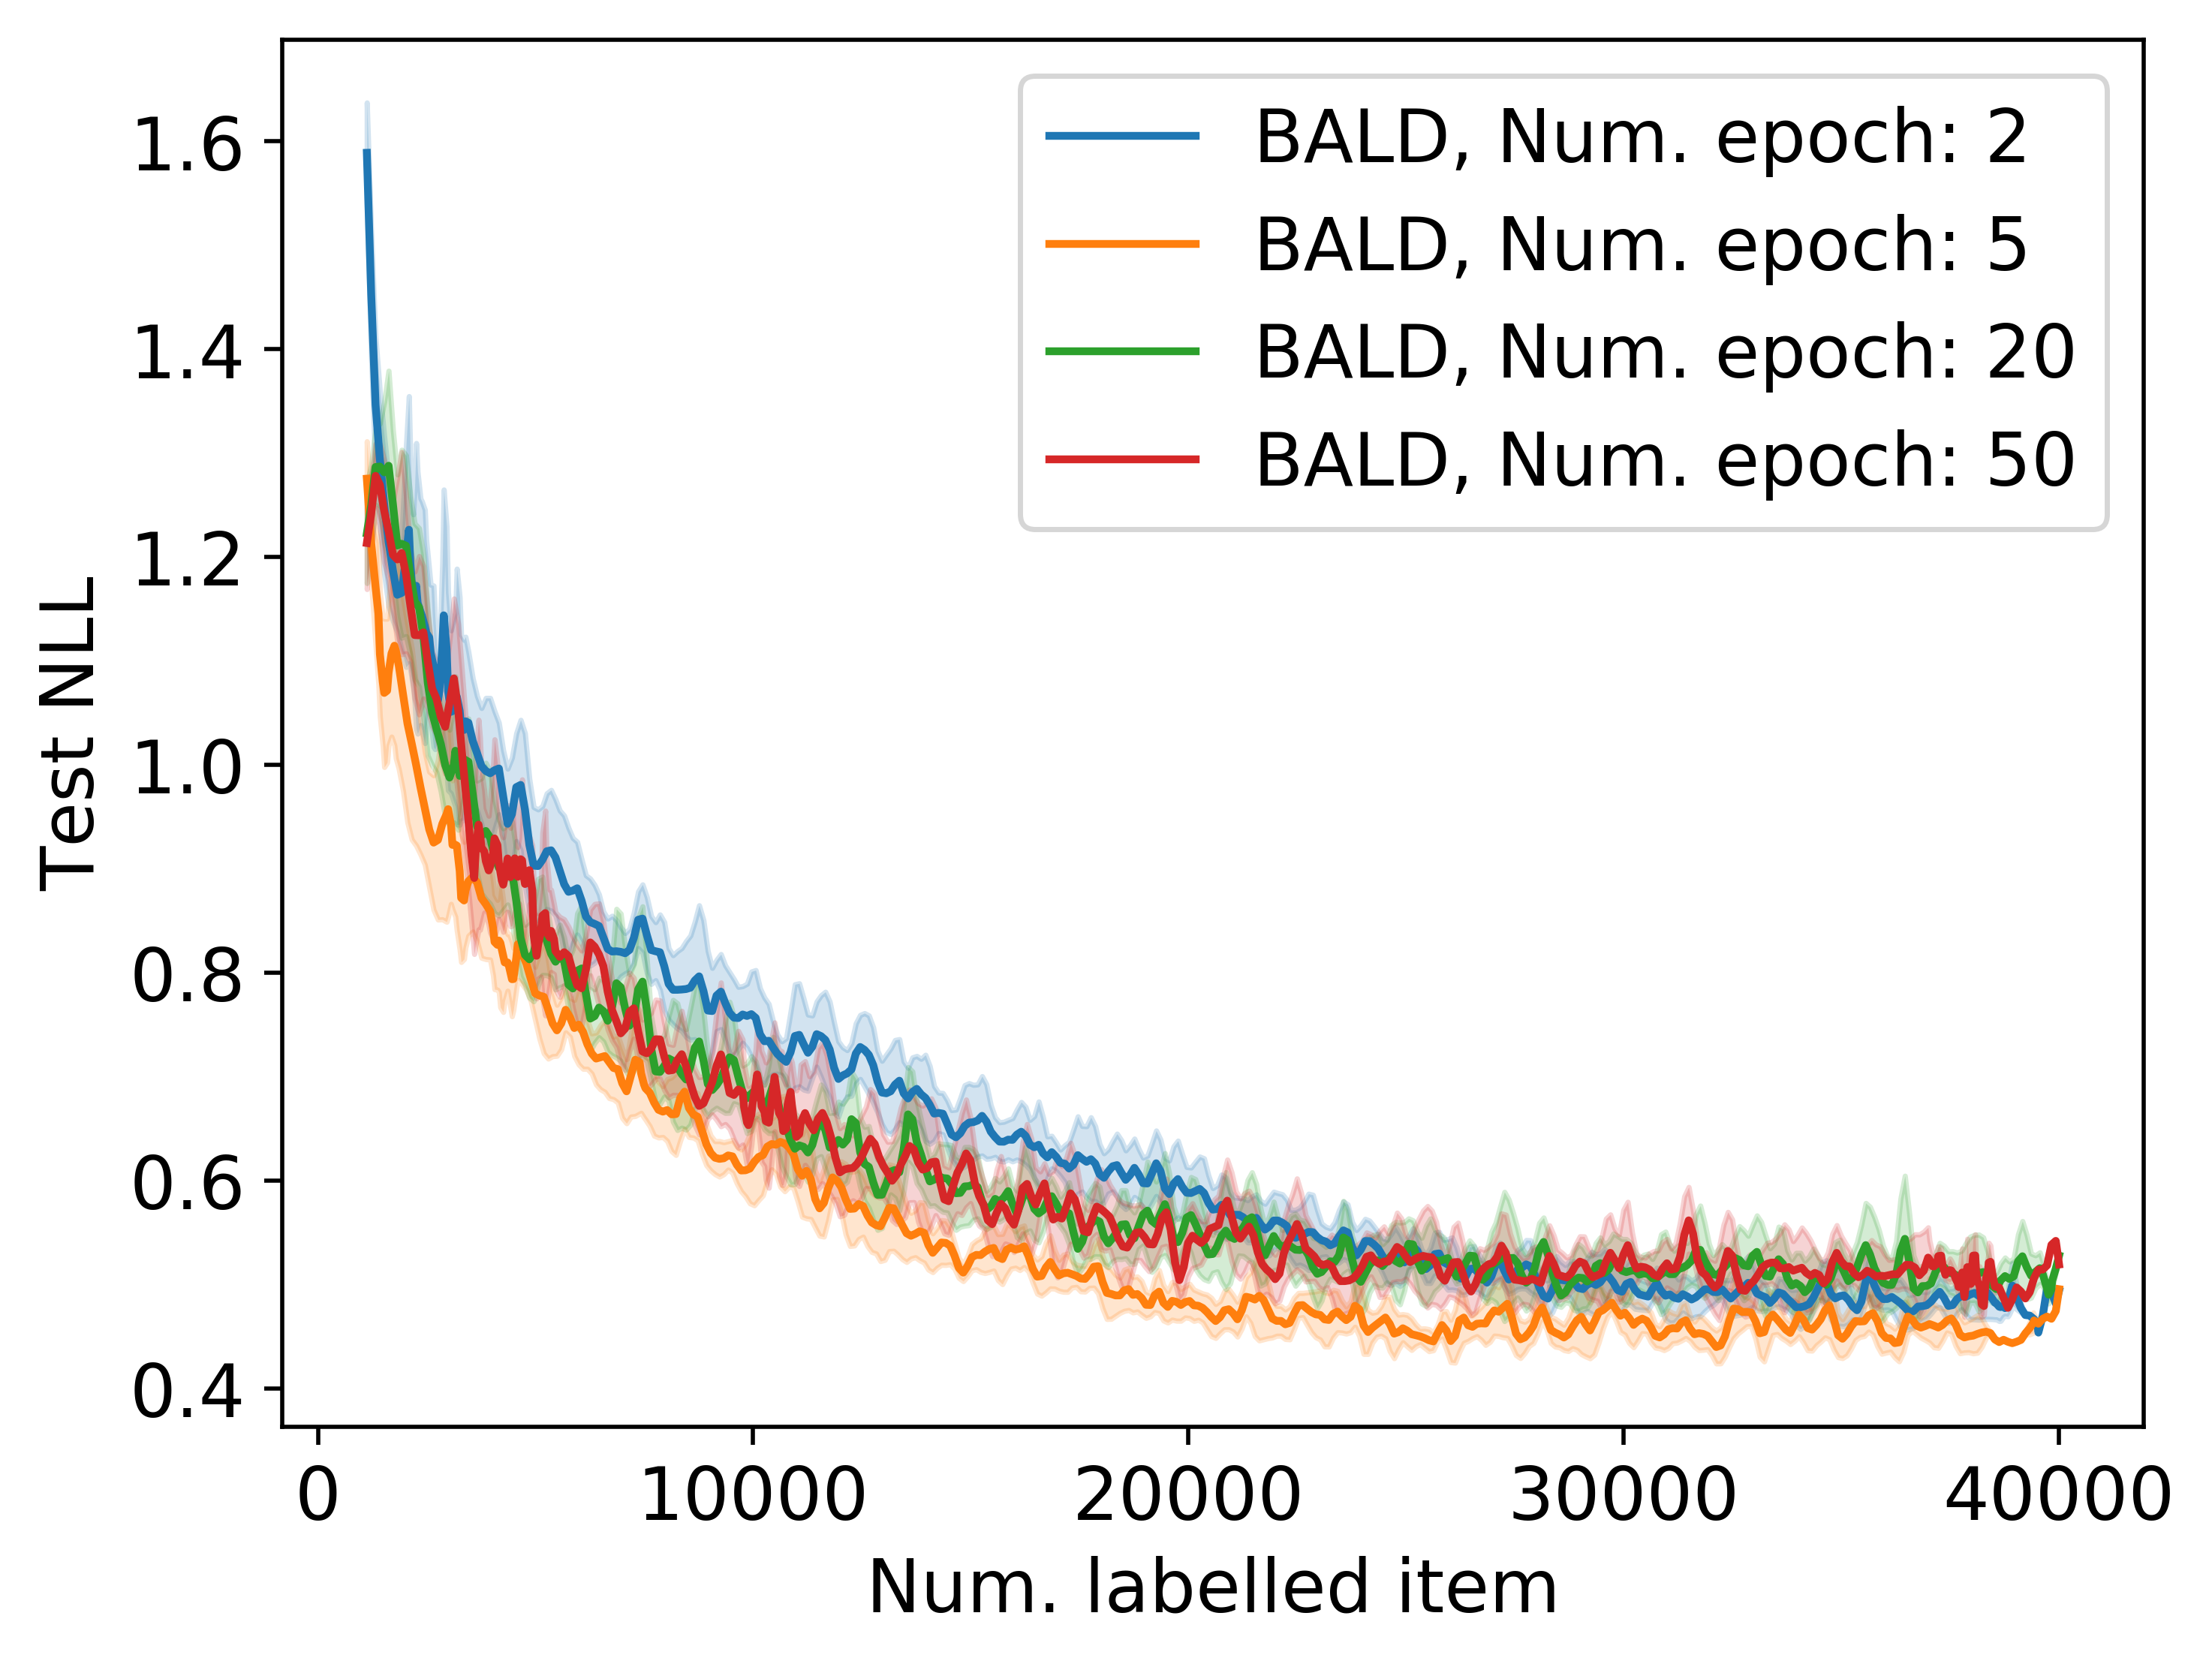
\includegraphics[width=0.35\textwidth]{fig/lrn_epoch.png}
    \caption{Effect of different training schedules. By comparing overfitted and underfitted models, we assess the impact of uncertainty quality on active learning. Performance averaged over 5 runs.}
    \label{fig:convergence}
\end{figure}


% \paragraph{Imbalanced datasets}

% How to deal with imbalanced datasets is an entire area of research \citep{krawczyk2016learning}, but little has been done to deal with it when we are not aware of the \textit{a priori} class distribution. In consequence, the active learning model may quickly overfit to the more popular classes and reduce the effectiveness of active learning procedure. From \citet{gal2017deep}, it is known that Bayesian active learning will favor underrepresented classes. But, we find the reported experiments to too simple. We  test this hypothesis in a controlled environment where we can set the amount of unrepresented classes. 

% In \tabref{fig:imbalanced}, we took the standard CIFAR100 dataset and we mimic an imbalanced dataset where few classes have a high number of examples. A class selected to be under represented sees its number of samples to be reduced by 90\%. When we increase the number of underrepresented classes, the gain of using MC-Dropout versus random sampling become more obvious. This is due to regions on the learned manifold associated with underrepresented classes to be highly uncertain. In consequence, these regions will be selected for labelling very early in the process.

% \begin{table}
%     \centering
%     \begin{tabular}{llll}
    
%     \toprule
%     Dataset size &         5000 &        10000 &        20000 \\
    
%     \hline
%   $\Delta =10$ \\
%     BALD &  4.39 \std{0.4} &  3.99 \std{0.01} &  3.57 \std{0.05} \\
%     Entropy &  4.71 \std{0.02} &  4.54 \std{0.07} &  3.94 \std{0.01} \\
%     Random &  4.52 \std{0.09} &  4.10 \std{0.03} &  3.71 \std{0.05} \\
%     \hline
%   $\Delta =25$ \\
%     BALD &  4.40 \std{0.03}	&4.04\std{0.03} &	3.61\std{0.08} \\
%     Entropy &  4.76 \std{0.02} &  4.68 \std{0.08} &   4.00 \std{0.01} \\
%     Random &  4.58 \std{0.08} &  4.18 \std{0.04} &  3.75 \std{0.01} \\
%     \hline 
%   $\Delta =50$ \\
%     BALD &  4.49 \std{0.08} &   4.07 \std{0.02} &   3.66 \std{0.04} \\
%     Entropy &  4.83 \std{0.04} &  4.60 \std{0.14} &  4.07 \std{0.28} \\
%     Random &  4.62 \std{0.03} &   4.21 \std{0.02} &   3.76 \std{0.04}
%     \end{tabular}
%     \caption{Effect of using active learning on imbalanced versions of CIFAR100. $\Delta$ is the number of class that contains 25\% of their data. From \citep{gal2017deep}, we know that BALD is robust to imbalanced datasets, but the study was not extensive. While BALD is robust to imbalanced datasets, the effect is catastrophic when using Entropy.  Performance averaged over 5 runs.}
%     \label{fig:imbalanced}
% \end{table}


% In this section, we investigated how common issues in deep learning are affecting active learning. While BALD is robust to data imbalance, it is highly affected by the annotation error or being under fitted.
In this section, we investigated the effect of two common deep learning pathologies in active learning. In summary, prior knowledge on the quality of the annotations and on how long to train the model, could help using active learning. 

\subsection{Efficient techniques for active learning}\label{techniques}

An important problem with current active learning pipelines is the delay between active learning steps. %In particular, at the beginning of the process, computing the uncertainty on the unlabelled pool of observations has a prohibitive cost. When the labelled dataset becomes large, then the cost of training the model becomes prohibitive. 
To make active learning efficient, we propose several techniques that maintain performance while speeding up the training or inference phases.

\paragraph{Query size}
An important hyper-parameter in batch active learning is to decide how many samples should be labelled at each active learning step \citep{gal2017deep, tsymbalov2019deeper}. %This parameter turns out to be vital to be set properly as \citet{tsymbalov2019deeper} as shown. 
In a real-world scenario, we can't ask the annotation team to wait between steps especially in a crowd-sourcing environment. %Of course, we do not want to label the whole pool of dataset in the next coming active learning step, and on the other extreme, we neither want to add only one sample label to the labelled subset of data. The first scenario would require labelling the whole dataset which is against the purpose of the whole framework and the latter will result in an exhaustively slow process which we obviously could not afford in a production setup. 
Therefore, there needs to be a configuration where we could benefit from a good uncertainty estimation quality and a reasonable runtime. We present our findings in \tabref{fig:query_size} where we tested this approach on CIFAR10. 
From our results, the query size does decreases performances, especially at 10,000 labels where the gap between BALD and Entropy is thinner as the query size grows.

\begin{table}
{\small
\begin{tabular}{llll}
\toprule
    Dataset size &          5000 &         10000 &         20000 \\
\midrule
\textbf{Random} &  0.71 \std{0.03} &  0.54 \std{0.01} &  0.42 \std{0.05} \\
\hline
   $\Q$=50 &                  &                  &                  \\
   \hline
            BALD &  0.59 \std{0.01} &  0.46 \std{0.05} &  0.34 \std{0.02} \\
         Entropy &  0.69 \std{0.06} &  0.55 \std{0.11} &  0.34 \std{0.00} \\
          \hline
  $\Q$=250 &                  &                  &                  \\
  \hline
            BALD &  0.61 \std{0.03} &  0.43 \std{0.01} &  0.35 \std{0.03} \\
         Entropy &  0.67 \std{0.05} &  0.49 \std{0.04} &  0.35 \std{0.00} \\
          \hline
  $\Q$=500 &                  &                  &                  \\
  \hline
            BALD &  0.61 \std{0.07} &  0.42 \std{0.02} &  0.36 \std{0.01} \\
         Entropy &  0.61 \std{0.07} &  0.47 \std{0.00} &  0.37 \std{0.00} \\
          \hline
 $\Q$=2000 &                  &                  &                  \\
 \hline
            BALD &  0.77 \std{0.05} &  0.53 \std{0.03} &  0.37 \std{0.03} \\
         Entropy &  0.87 \std{0.01} &  0.52 \std{0.07} &  0.35 \std{0.01} \\
\bottomrule
\end{tabular}}



    \centering
    \caption{Effect of increasing the query size $\Q$ on CIFAR10. Performance averaged over 5 runs. BALD is weaker when used with a large query size, making Entropy competitive.}
    \label{fig:query_size}
\end{table}

\paragraph{Limit pool size}

The most time-consuming part of active learning is the uncertainty estimation step. In particular, this step is expensive when using techniques that require Monte-Carlo sampling such as MC-Dropout or Bayesian neural networks. 
Of course, this problem is embarrassingly parallel, but for low-budget deployment, one has not access to the resources required to parallelize this task cheaply.
A simple idea to solve this is to randomly select unlabelled samples from the pool instead of using the entire pool. We test this idea by varying the number of samples selected for uncertainty estimation. 
%In \figref{fig:pool_size}, we show that there is no difference between choosing between the entire pool or less than 25\%. This shows that one can heavily speed up the inference phase by limiting the size of the pool
From our experiments (figure in Annex), we show that the performance is not affected when using less than 25\% of the pool. By doing this, we can speed up this phase by a factor of 3.

In this section, we proposed two approaches to make active learning usable in production. First, we can increase the query size higher than previously used in the literature. Second, we can select the next batch using a small subset of the pool.

% \begin{figure}
%     \centering
%     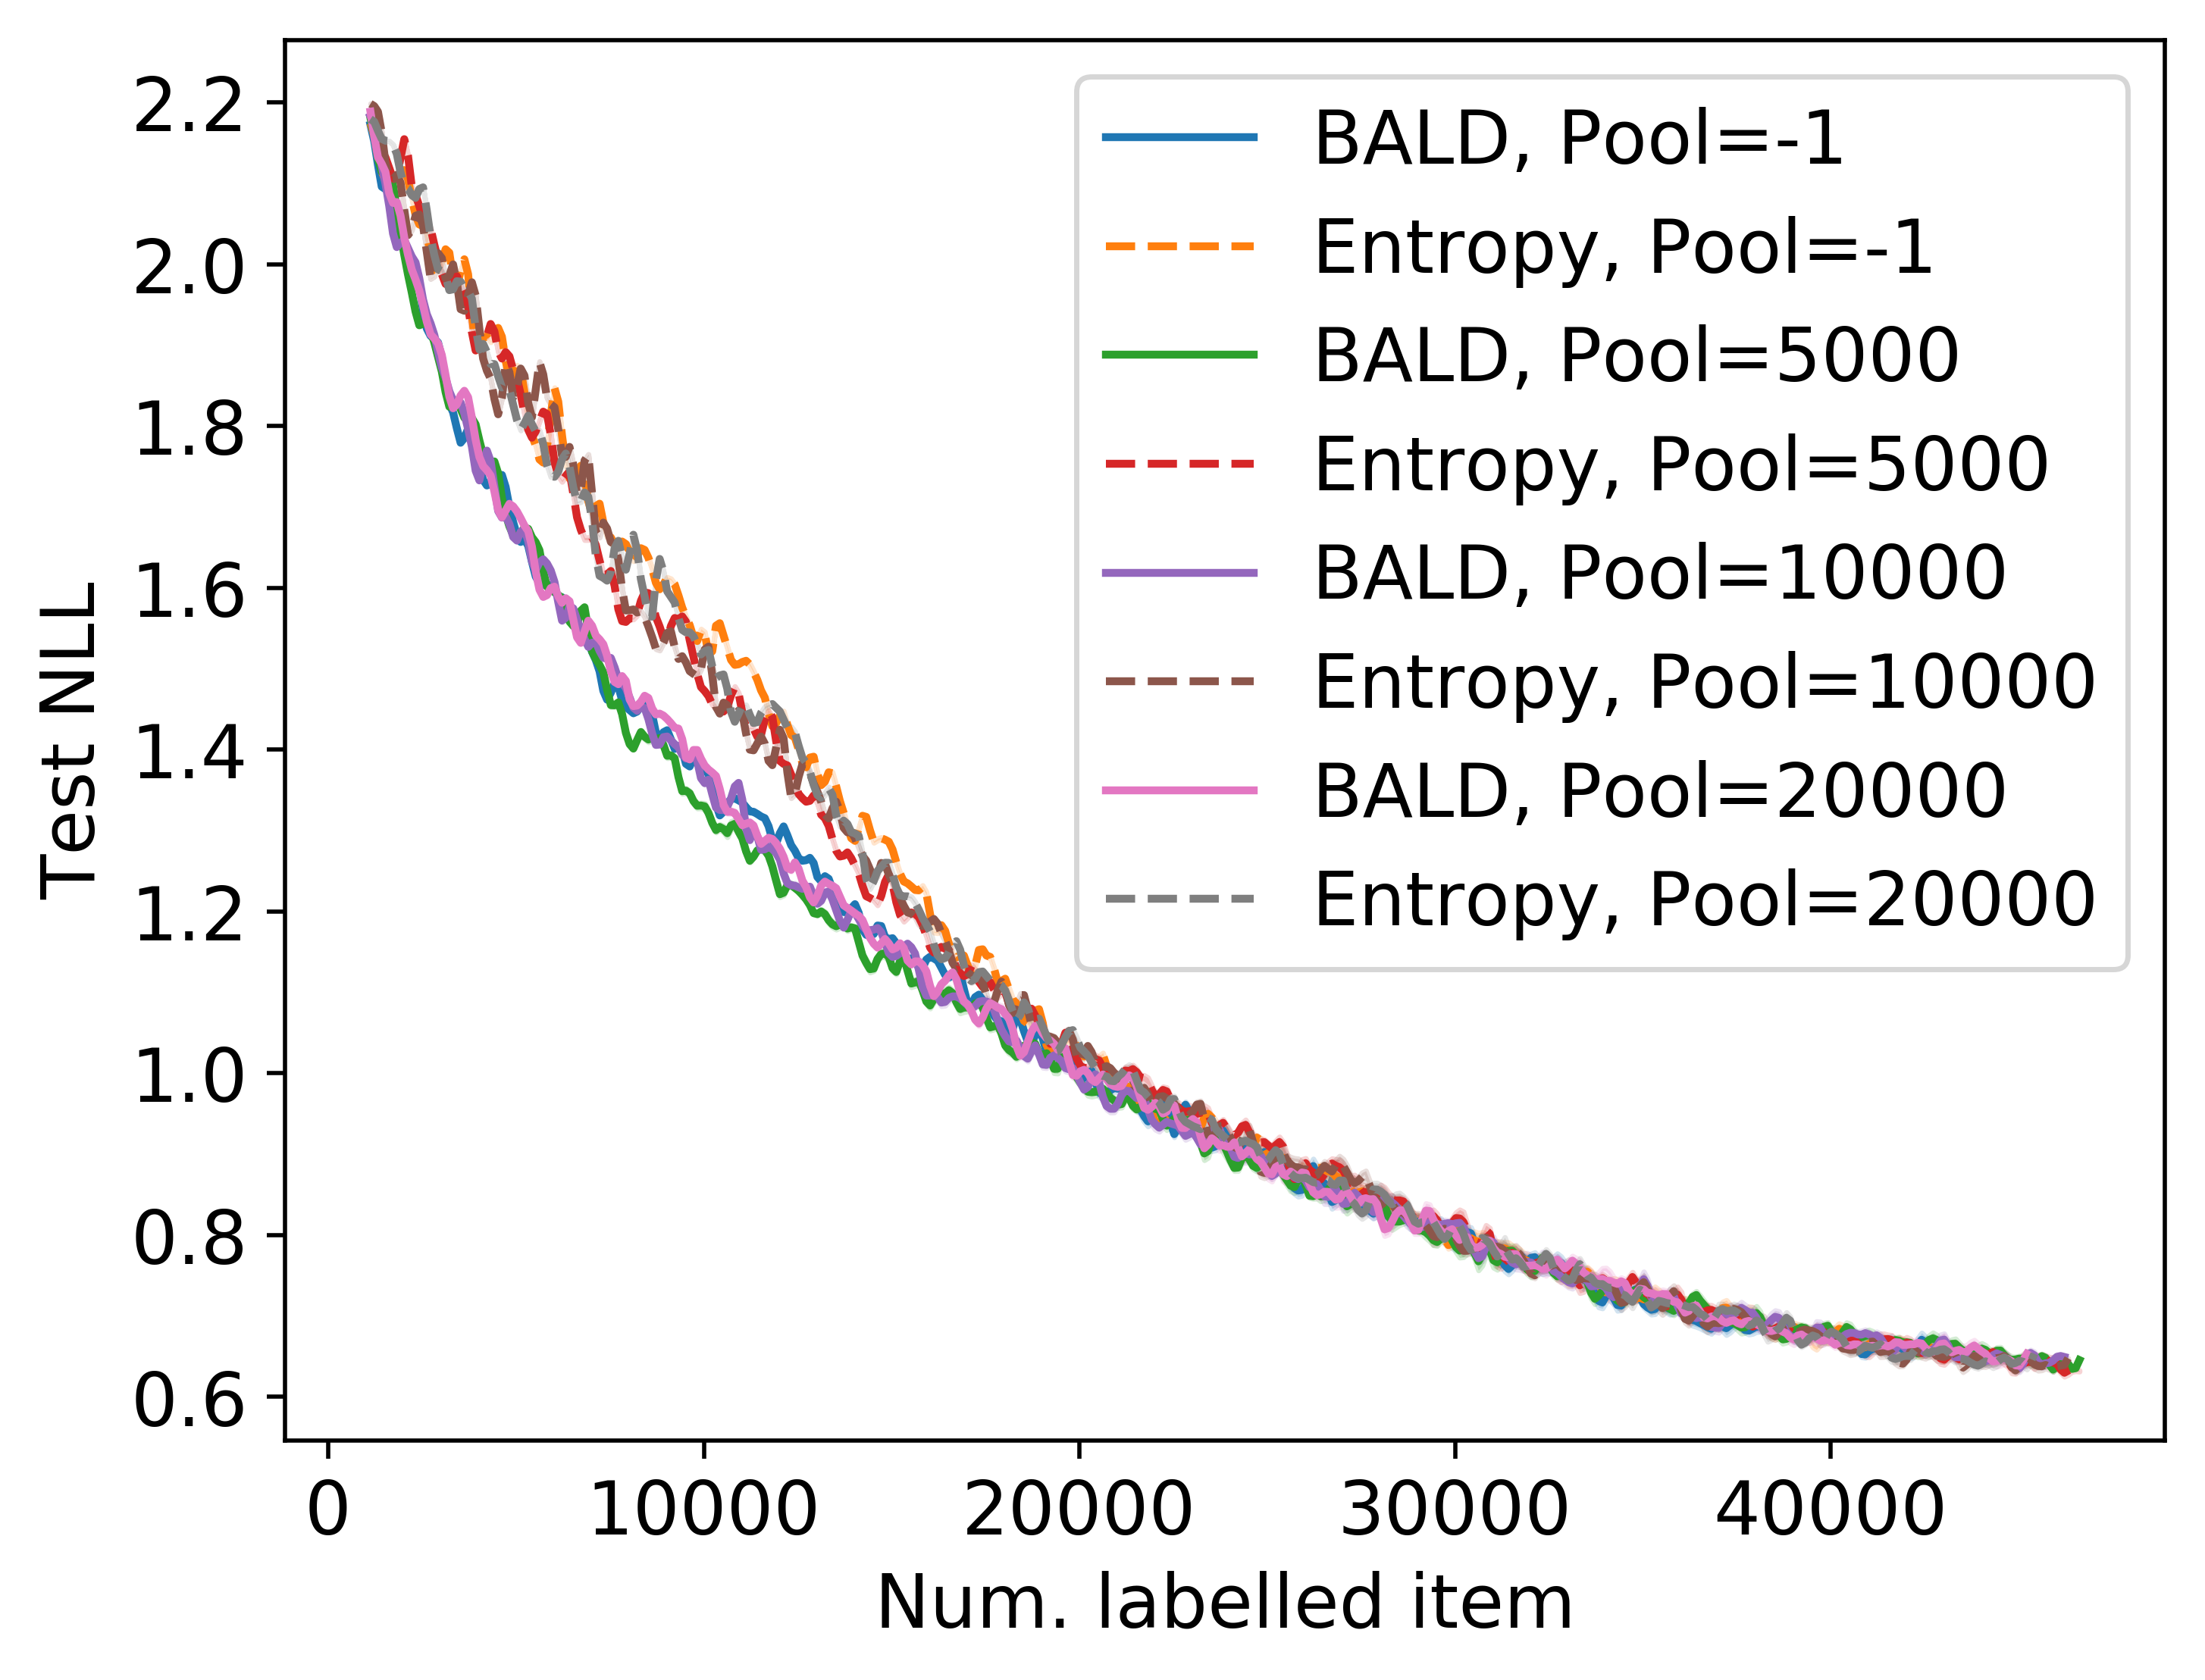
\includegraphics[width=0.4\textwidth]{fig/pol_size.png}
%     \caption{Effect of reducing the size of the pool on CIFAR10. \textbf{-1} indicates no reduction. For all heuristics, the performance is not affected by the size of the pool showing that AL can be efficient when tuned properly.  Performance averaged over 5 runs.}
%     \label{fig:pool_size}
% \end{figure}

\section{Case study: Mio-TCD}

Few datasets have been proposed to mimic a "real-world" situation where the dataset suffers from labelling noise, duplicates, or imbalanced datasets. Mio-TCD \citep{luo2018mio} has been recently proposed to showcase these issues. The dataset contains 500,000 samples split into 11 classes with heavy class imbalance. For example, the training set contains 50\% \textit{Cars} and 20\% \textit{Background}. 

\paragraph{Benefits of active learning.}
As shown in \citet{gal2017deep} (and further in Annex), active learning helps when used on imbalanced data. We can verify this, by comparing the performance of underrepresented classes in Mio-TCD. From the current leader board, we can select two difficult classes: \textit{Single-Unit Truck, and Bicycle}. We use the same setup as before, but limit the size of the pool to 20,000 samples. %Comparing the results in \figref{fig:standard}, BALD is clearly superior which further validates the need for better benchmarks in active learning.



% \subsubsection{Adding random noise to the selection}

% We first analyze the impact of the proposition of \citet{dasgupta2011two} to add noise when selecting the next samples to label.
% In this highly imbalanced dataset, we make the hypothesis that it would be highly valuable as it is likely that some classes are not represented in the initial random sampling. Furthermore, at each active learning step, the pool of unlabelled data would be ranked based on model uncertainty before selecting the samples to be labeled. In this setting, two classes can be highly confused and ,depending on the selection process, still be highly confident predictions.

% Furthermore, as \citet{lowell2019practical} has demonstrated, datasets labelled using active learning are good to train deep learning models, but not so much when training models from different paradigms. % ICML CUT new paper By adding noise to the selection, we hope to remove some part of the selection bias added to the dataset.
\begin{figure}
    \centering
    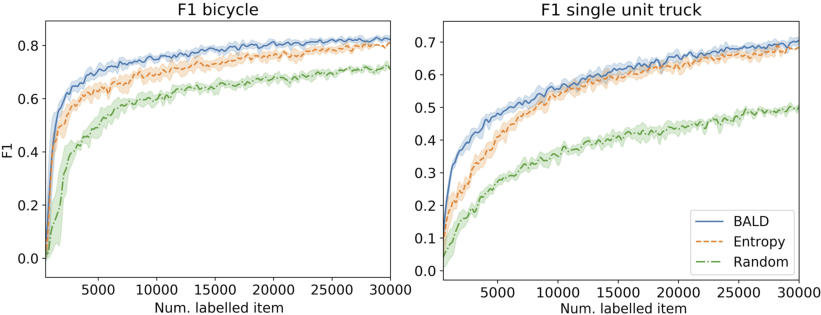
\includegraphics[width=0.5\textwidth]{fig/F1_Miotcd_top.pdf}
    \caption{Performance of different active learning procedures on Mio-TCD. While any active learning method is strong against random, BALD is especially strong at the beginning of the labelling process.  Performance averaged over 5 runs.}
    \label{fig:mioclasses}
\end{figure}
% However, what model chooses to be most valuable in the next round of training is not necessarily diverse enough and could be concentrated on part of the data which is simply harder to decode for the model. Continuing in adding samples solely based on model uncertainty feedback, could eventually teach the model to learn the most uncertain part of the data while the least uncertain part do not get any representation in the bigger scale and hence model would fail in learning the whole data distribution\cite{dasgupta2011two}. 

In \figref{fig:mioclasses}, we present the F1 scores for the two most difficult classes. One can clearly see the impact of using active learning in this setting. With active learning, underrepresented classes are quickly selected and get decent performance. In addition, the performance for the most populous class \textit{Cars} stays similar across acquisition functions (figure in Annex). 

%ICML CUT no gain actually Given the percentage of noise, we randomly swap samples from the ranked set of pool. For example, choosing to label 100 samples at each active learning step with 10\% noise means that 90 data point will be labelled based on model uncertainty decision and 10 data points will be labelled randomly. Using this method is especially useful for \textit{entropy} which is weaker than BALD. On the contrary, BALD is not affected by this method, but it does not get hurt it either.

This experiment shows that using active learning on non-academic datasets is highly beneficial and the need for the active learning community to use new benchmarks to compare methods.





\section{Conclusion}

In this paper, we have investigated the impact of uncleaned data on deep active learning models used for active learning. We also propose several techniques to make active learning usable in a real-world environment. Subsequently, we test our findings on a real-world dataset Mio-TCD, showing that active learning can be used in this setting.  As a result of this study, we introduce our newly released Bayesian active learning library which can be useful to both researchers and developers (see Annex).


In summary, we show that active learning can be used in a production setting on real data with success. We hope this work can fasten the application of active learning on real-world projects and improve the quality of annotation by getting more information per sample. Interesting areas of research include the study of the interaction between the human and the machine during a labelling task.

\clearpage
\bibliography{example_paper}
\bibliographystyle{icml2020}
% For submission, needs to be 2 documents and then concat together.
\appendix
%%%%%%%% ICML 2020 EXAMPLE LATEX SUBMISSION FILE %%%%%%%%%%%%%%%%%

\documentclass{article}
\usepackage{times}
\usepackage{epsfig}
\usepackage{graphicx}
\usepackage{amsmath}
\usepackage{amssymb}
\usepackage{times}
\usepackage{epsfig}
\usepackage{graphicx}
\usepackage{amsmath}
\usepackage{amssymb}
% Include other packages here, before hyperref.
\usepackage{xcolor}
\usepackage[ruled,vlined,onelanguage]{algorithm2e}
\usepackage{setspace}
\usepackage{collcell}
\usepackage{xr}
\usepackage{natbib}
\usepackage{multirow}
\usepackage{subcaption}
\usepackage{mathtools}
\usepackage{colortbl,dcolumn}
\usepackage{algorithm2e}

% Include other packages here, before hyperref.

% If you comment hyperref and then uncomment it, you should delete
% egpaper.aux before re-running latex.  (Or just hit 'q' on the first latex
% run, let it finish, and you should be clear).
\usepackage[pagebackref=true,breaklinks=true,letterpaper=true,colorlinks,bookmarks=false]{hyperref}

% \cvprfinalcopy % *** Uncomment this line for the final submission

\def\cvprPaperID{****} % *** Enter the CVPR Paper ID here
\def\httilde{\mbox{\tt\raisebox{-.5ex}{\symbol{126}}}}

\newcommand{\todo}[1]{{\color{blue}TODO #1}}
\newcommand{\toref}[1]{{\color{red}REF #1 }}
\newcommand{\registered}{\textsuperscript{\tiny\textregistered}}
%\newcommand{\etal}{\textit{et al.}}
\renewcommand{\eqref}[1]{\hyperref[#1]{Eq.\ \ref*{#1}}}
\newcommand{\figref}[1]{\hyperref[#1]{Fig.\ \ref*{#1}}}
\newcommand{\tabref}[1]{\hyperref[#1]{Table\ \ref*{#1}}}
\newcommand{\secref}[1]{\hyperref[#1]{Section\ \ref*{#1}}}
\newcommand{\algoref}[1]{\hyperref[#1]{Algorithm\ \ref*{#1}}}
\newcolumntype{C}[1]{>{\centering}m{#1}}
\newcommand{\N}{{\cal N}}
\newcommand{\std}[1]{ \normalfont \color{darkgray}\footnotesize{$\pm$#1} }

% SYMBOL
\newcommand{\E}{{\mathbb E}}

\hypersetup{
    colorlinks=true,
    linkcolor=blue,
    filecolor=magenta,      
    urlcolor=blue,
}

\urlstyle{same}

% Recommended, but optional, packages for figures and better typesetting:
\usepackage{microtype}
\usepackage{booktabs} % for professional tables

% hyperref makes hyperlinks in the resulting PDF.
% If your build breaks (sometimes temporarily if a hyperlink spans a page)
% please comment out the following usepackage line and replace
% \usepackage{icml2020} with \usepackage[nohyperref]{icml2020} above.
\usepackage{hyperref}

% Attempt to make hyperref and algorithmic work together better:
\newcommand{\theHalgorithm}{\arabic{algorithm}}

% Use the following line for the initial blind version submitted for review:
%\usepackage{icml2020}

% If accepted, instead use the following line for the camera-ready submission:
\usepackage[accepted]{icml2020}

% The \icmltitle you define below is probably too long as a header.
% Therefore, a short form for the running title is supplied here:
\icmltitlerunning{Bayesian active learning for production. Supplementary Material}

\begin{document}

\twocolumn[
\icmltitle{Supplementary Material}]

\section{Implementation details}
Our methodology is as follows. We train a VGG-16 \citep{zhang2015accelerating} pretrained on ImageNet~\citep{imagenet_cvpr09}. Our initial training set contains 500 samples. We estimate the uncertainty using 20 MC samples and label the 100 most uncertain elements. Following \citet{gal2017deep}, we reset the weights to their initial value between steps. 

\section{Imbalanced datasets}
 
How to deal with imbalanced datasets is an entire area of research \citep{krawczyk2016learning}, but little has been done to deal with it when we are not aware of the \textit{a priori} class distribution. In consequence, the active learning model may quickly overfit to the more popular classes and reduce the effectiveness of active learning procedure. From \citet{gal2017deep}, it is known that Bayesian active learning will favor underrepresented classes. But, we find the reported experiments to be too simple. We  test this hypothesis in a controlled environment where we can set the number of unrepresented classes. 

In \tabref{fig:imbalanced}, we took the standard CIFAR100 dataset and we mimic an imbalanced dataset where few classes have a high number of examples. A class selected to be underrepresented sees its number of samples to be reduced by 75\%. When we increase the number of underrepresented classes, the gain of using MC-Dropout versus random sampling becomes more obvious. This is due to regions on the learned manifold associated with underrepresented classes to be highly uncertain. In consequence, these regions will be selected for labelling very early in the process.

% In this section, we investigated how common issues in deep learning are affecting active learning. While BALD is robust to data imbalance, it is highly affected by the annotation error or being under fitted.


\begin{table}
    \centering
    \begin{tabular}{llll}
    
    \toprule
    Dataset size &         5000 &        10000 &        20000 \\
    
    \hline
   $\Delta =10$ \\
    BALD &  4.39 \std{0.4} &  3.99 \std{0.01} &  3.57 \std{0.05} \\
    Entropy &  4.71 \std{0.02} &  4.54 \std{0.07} &  3.94 \std{0.01} \\
    Random &  4.52 \std{0.09} &  4.10 \std{0.03} &  3.71 \std{0.05} \\
    \hline
   $\Delta =25$ \\
    BALD &  4.40 \std{0.03}	&4.04\std{0.03} &	3.61\std{0.08} \\
    Entropy &  4.76 \std{0.02} &  4.68 \std{0.08} &   4.00 \std{0.01} \\
    Random &  4.58 \std{0.08} &  4.18 \std{0.04} &  3.75 \std{0.01} \\
    \hline 
   $\Delta =50$ \\
    BALD &  4.49 \std{0.08} &   4.07 \std{0.02} &   3.66 \std{0.04} \\
    Entropy &  4.83 \std{0.04} &  4.60 \std{0.14} &  4.07 \std{0.28} \\
    Random &  4.62 \std{0.03} &   4.21 \std{0.02} &   3.76 \std{0.04} \\
    \end{tabular}
    \caption{Effect of using active learning on imbalanced versions of CIFAR100. $\Delta$ is the number of class that contains 25\% of their data. From \citep{gal2017deep}, we know that BALD is robust to imbalanced datasets, but the study was not extensive. While BALD is robust to imbalanced datasets, the effect is catastrophic when using Entropy.  Performance averaged over 5 runs.}
    \label{fig:imbalanced}
\end{table}

\section{Effect of convergence}

In \figref{fig:active_gain}, we computed the difference in performance between BALD and random. We call this measure the \textit{Active gain} $= NLL_{Random} - NLL_{BALD}$. When using an underfitted model, the gain goes negative i.e. you would be better to use random selection.

\begin{figure}
    \centering
    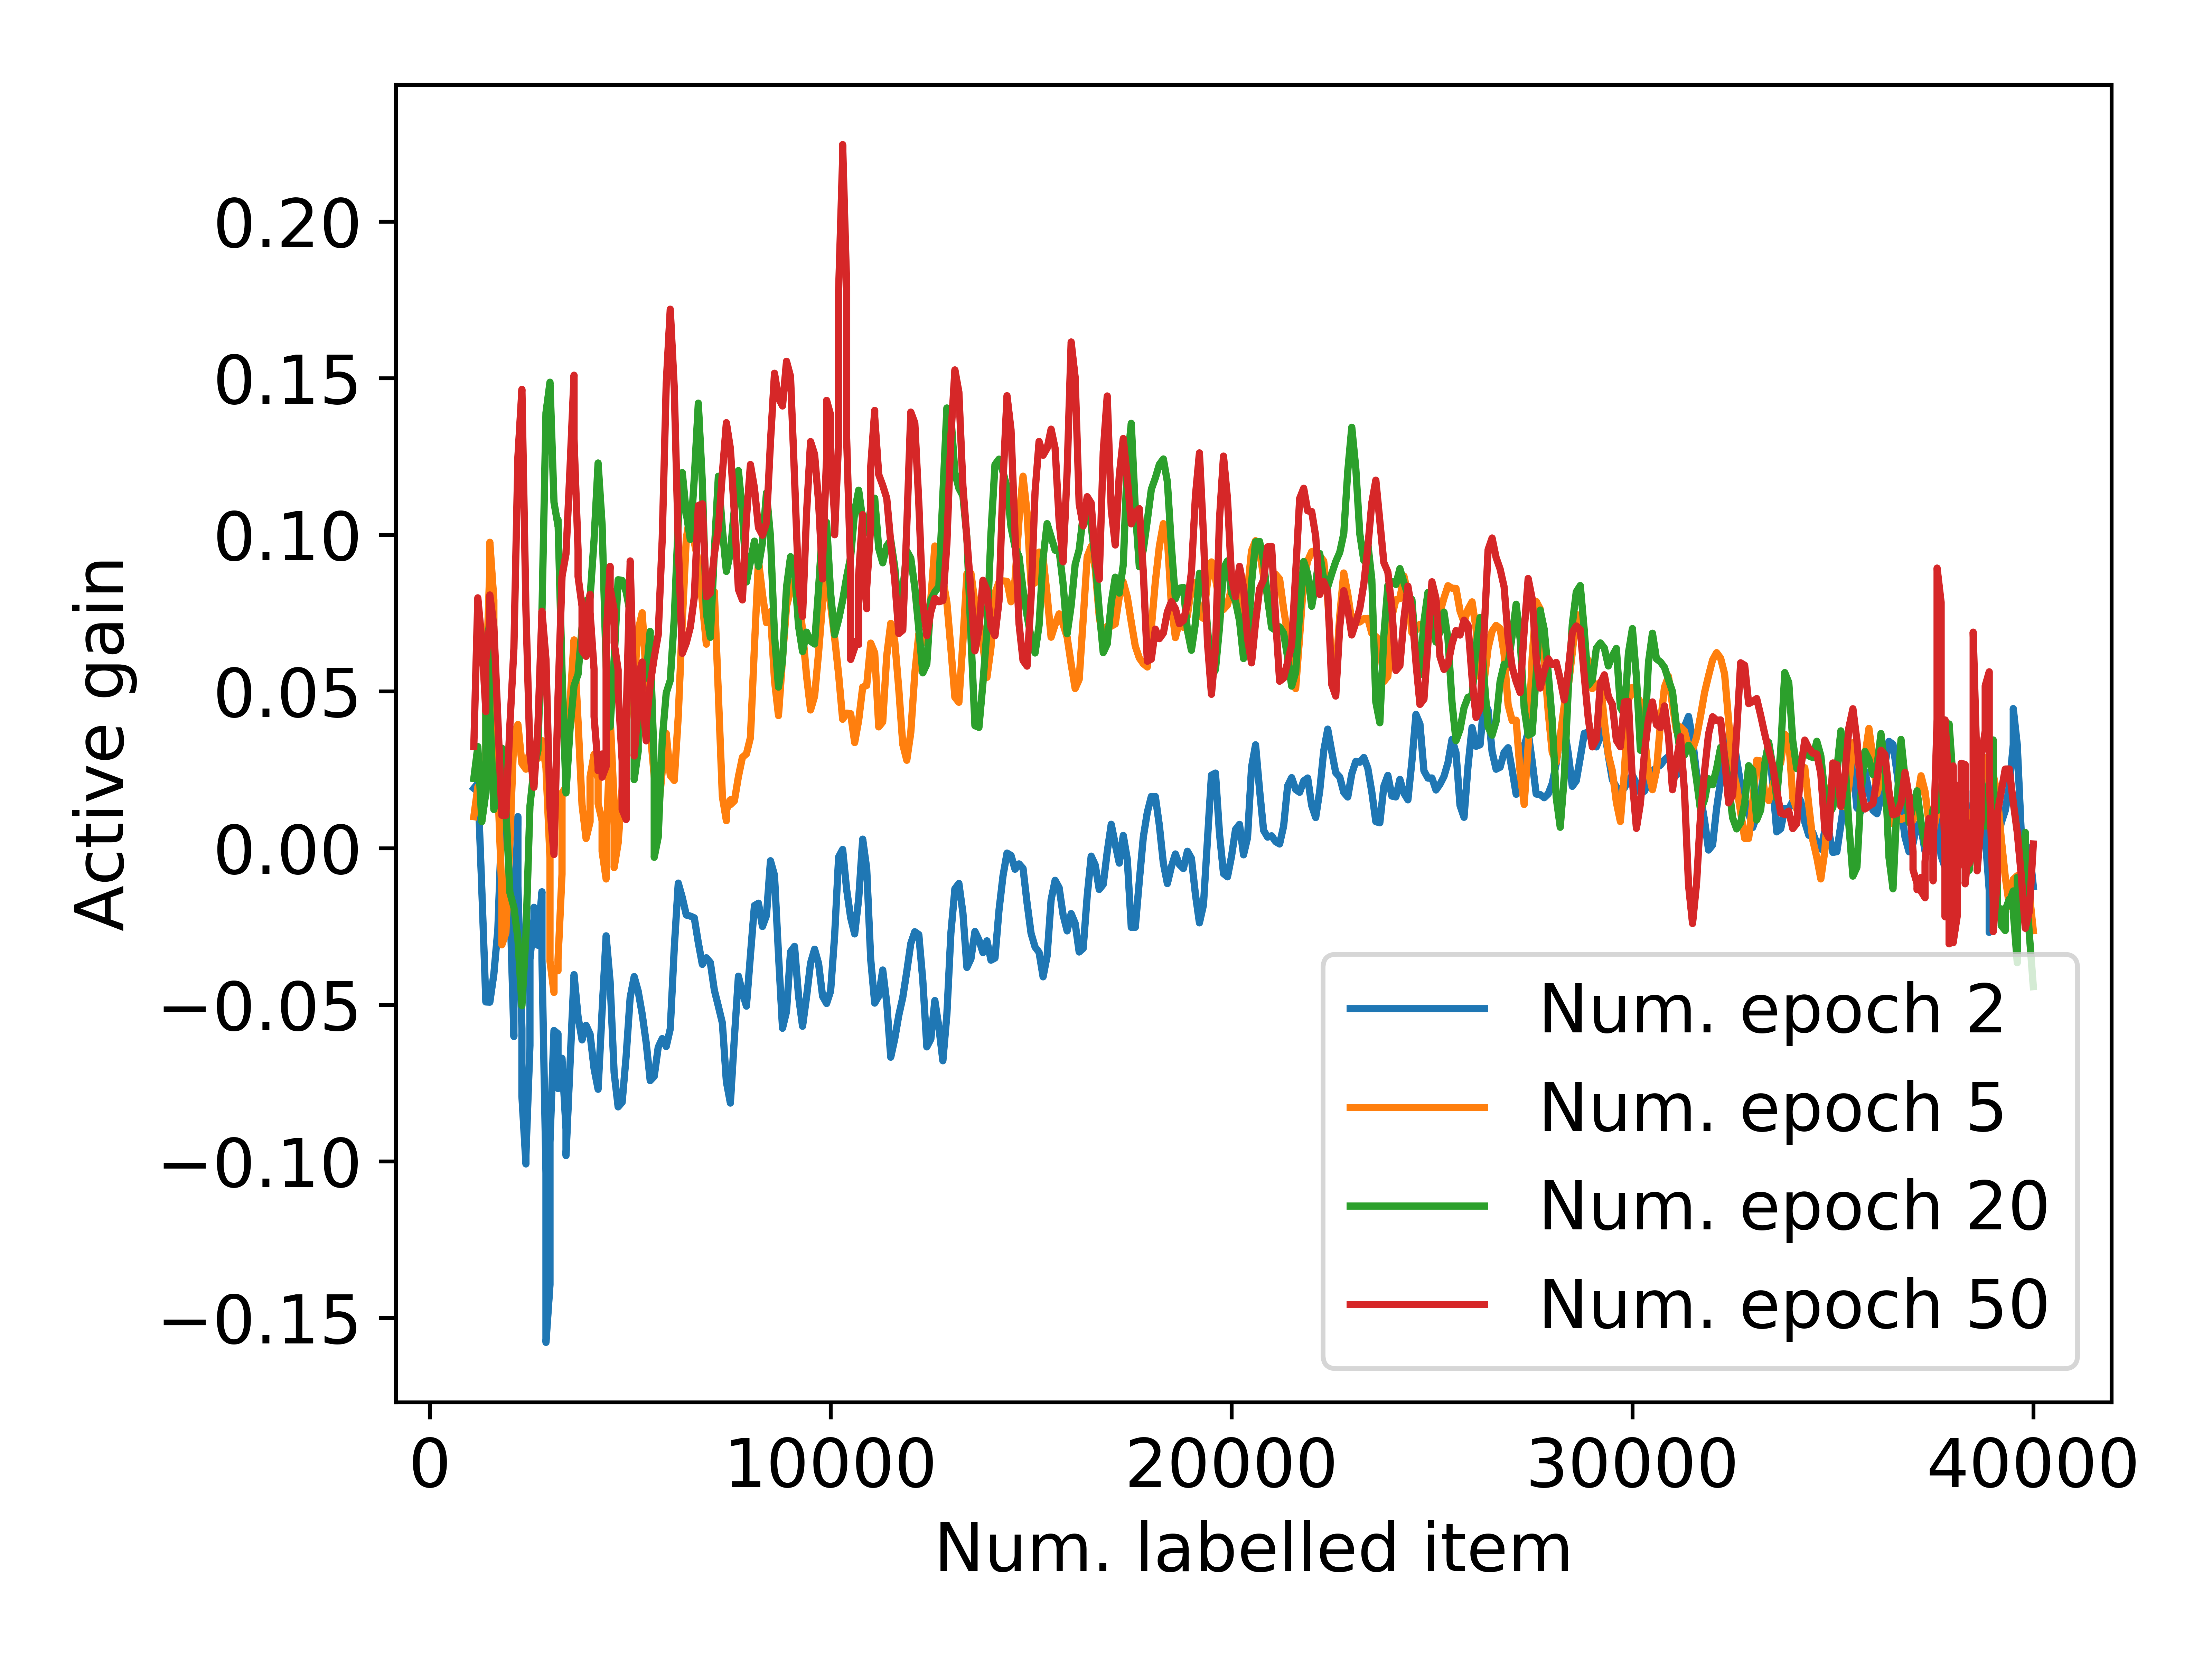
\includegraphics[width=0.5\textwidth]{fig/active_gain.png}
    \caption{Gain of using active learning when varying the number of training epochs. An underfitted model will cause harm to the model training and in this case, just using random would've been better.}
    \label{fig:active_gain}
\end{figure}

\section{Effect of reducing the pool size}
As part of the experiments, we test whether limiting the pool size would affect the performance of active learning. Our experiments in  \figref{fig:pool_size} show that whether to calculate the uncertainty for the whole pool data or a randomly selected subset, the performance of active learning is not affected. This leads to an the interesting outcome of limiting the uncertainty calculations (which is the most expensive part of an active learning loop) in production setup for faster active learning loops.

\begin{figure}
    \centering
    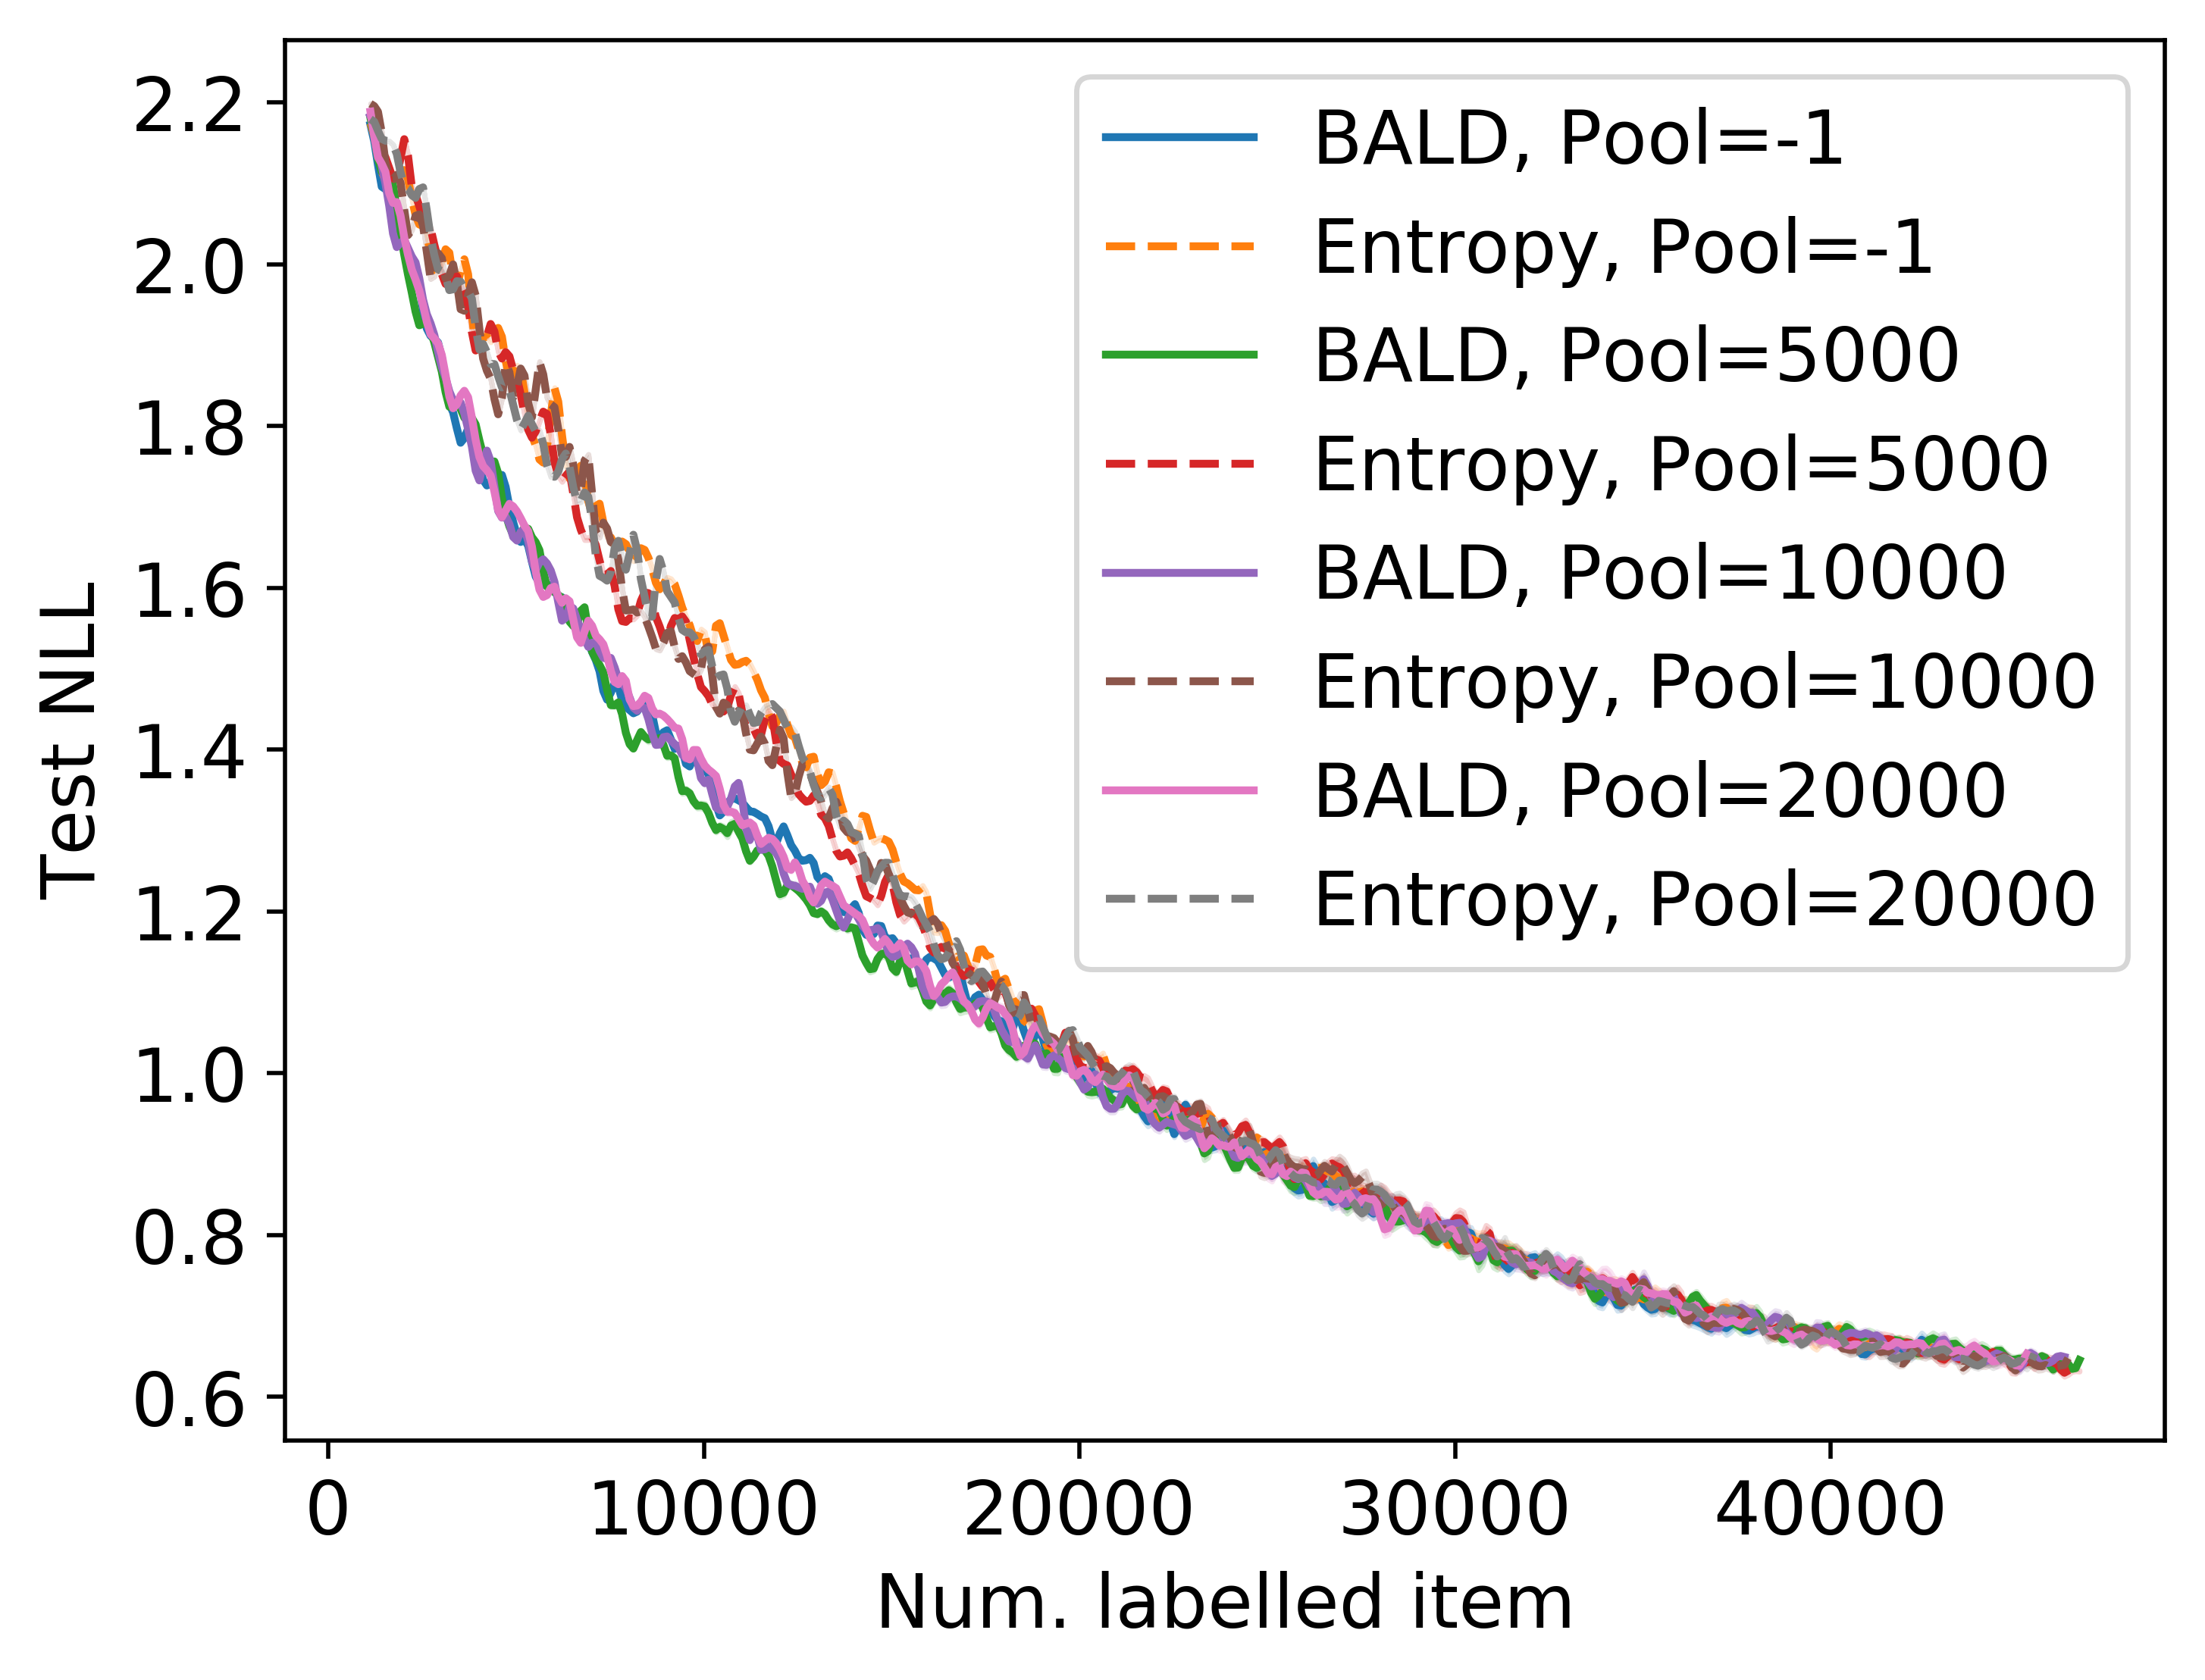
\includegraphics[width=0.4\textwidth]{fig/pol_size.png}
    \caption{Effect of reducing the size of the pool on CIFAR100. \textbf{-1} indicates no reduction. For all heuristics, the performance is not affected by the size of the pool showing that AL can be efficient when tuned properly.  Performance averaged over 5 runs.}
    \label{fig:pool_size}
\end{figure}

\begin{figure}
    \centering
    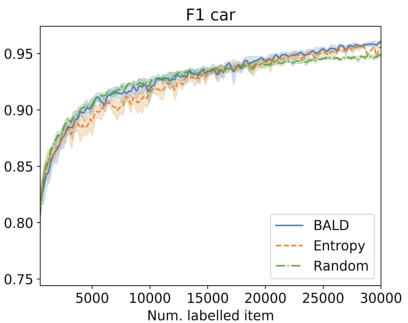
\includegraphics{fig/F1_Mio_tcd_annex.pdf}
    \caption{\textbf{F1 for the class \textit{car}}. BALD is great for underrepresented classes while not affecting more popular classes. Entropy decreases the performance on this class.}
    \label{fig:miotcd}
\end{figure}


\section{Bayesian active learning Library (BaaL)}

All the experiments in this paper have done using our publicly available Bayesian active learning library.  The goal of this library is to provide an easy to use but complete setup to test active learning on any project with few lines of code. We included features that current active learning libraries do not support. In particular, Bayesian methods such as MC-Dropout or Coresets are not widely available and there is no standard implementation of the active learning loop. Furthermore, research codebases are often hard to read and hard to maintain. Our proposed unified API could satisfy both research and industrial users.

 Our recently published open-source package named BaaL, aims at accelerating the transition from research to production. The core philosophy behind our library is to provide researchers with a well-designed API so that they focus on their novel idea and not on technical details. Our library proposes a task-agnostic system where one can mix-and-match any set of acquisition functions and uncertainty estimation methods.
The library consists of three main components:
\begin{enumerate}
    \item Dataset management to keep track and manage the labelled data $D_L$ and the unlabelled data $D_U$.
    \item Bayesian Methods i.e. MC-Dropout, MC-DropConnect and so on.
    \item Acquisition functions i.e. BALD, BatchBALD, Entropy and more.
\end{enumerate}

We provide full support for Pytorch \cite{paszke2017automatic} deep learning modules but our acquisition functions which are the most important part of active learning is implemented in  Numpy\cite{oliphant2006guide} and hence can be used on any platform. Our Data management module keeps track of what is labelled and what is unlabelled. We also provide facilitator methods to label a data point, update the pool of unlabelled data, and to randomly label a portion of the dataset. In our Bayesian module, we provide utilities to make any Pytorch model Bayesian with a single instruction. We also provide training, testing, and active learning loops that facilitate the active training procedure. Our acquisition functions are up-to-date with state-of-the-art methods. We provide easy to follow tutorials (https://baal.readthedocs.io/en/latest/) for each section of the library so that the user understands how each component works. Finally, our library is a member of Pytorch Ecosystem, which is reserved for libraries with outstanding documentation.

Our road-map has been indicated in the repository. Our current focus will include model calibration and semi-supervised learning. As more researchers contribute their methods to our library, we aim to become the standard Bayesian active learning library.

\end{document}
\end{document}



% This document was modified from the file originally made available by
% Pat Langley and Andrea Danyluk for ICML-2K. This version was created
% by Iain Murray in 2018, and modified by Alexandre Bouchard in
% 2019 and 2020. Previous contributors include Dan Roy, Lise Getoor and Tobias
% Scheffer, which was slightly modified from the 2010 version by
% Thorsten Joachims & Johannes Fuernkranz, slightly modified from the
% 2009 version by Kiri Wagstaff and Sam Roweis's 2008 version, which is
% slightly modified from Prasad Tadepalli's 2007 version which is a
% lightly changed version of the previous year's version by Andrew
% Moore, which was in turn edited from those of Kristian Kersting and
% Codrina Lauth. Alex Smola contributed to the algorithmic style files.

%%%%%%%% ICML 2020 EXAMPLE LATEX SUBMISSION FILE %%%%%%%%%%%%%%%%%

\documentclass{article}
\usepackage{times}
\usepackage{epsfig}
\usepackage{graphicx}
\usepackage{amsmath}
\usepackage{amssymb}
\usepackage{times}
\usepackage{epsfig}
\usepackage{graphicx}
\usepackage{amsmath}
\usepackage{amssymb}
% Include other packages here, before hyperref.
\usepackage{xcolor}
\usepackage[ruled,vlined,onelanguage]{algorithm2e}
\usepackage{setspace}
\usepackage{collcell}
\usepackage{xr}
\usepackage{natbib}
\usepackage{multirow}
\usepackage{subcaption}
\usepackage{mathtools}
\usepackage{colortbl,dcolumn}
\usepackage{algorithm2e}

% Include other packages here, before hyperref.

% If you comment hyperref and then uncomment it, you should delete
% egpaper.aux before re-running latex.  (Or just hit 'q' on the first latex
% run, let it finish, and you should be clear).
\usepackage[pagebackref=true,breaklinks=true,letterpaper=true,colorlinks,bookmarks=false]{hyperref}

% \cvprfinalcopy % *** Uncomment this line for the final submission

\def\cvprPaperID{****} % *** Enter the CVPR Paper ID here
\def\httilde{\mbox{\tt\raisebox{-.5ex}{\symbol{126}}}}

\newcommand{\todo}[1]{{\color{blue}TODO #1}}
\newcommand{\toref}[1]{{\color{red}REF #1 }}
\newcommand{\registered}{\textsuperscript{\tiny\textregistered}}
%\newcommand{\etal}{\textit{et al.}}
\renewcommand{\eqref}[1]{\hyperref[#1]{Eq.\ \ref*{#1}}}
\newcommand{\figref}[1]{\hyperref[#1]{Fig.\ \ref*{#1}}}
\newcommand{\tabref}[1]{\hyperref[#1]{Table\ \ref*{#1}}}
\newcommand{\secref}[1]{\hyperref[#1]{Section\ \ref*{#1}}}
\newcommand{\algoref}[1]{\hyperref[#1]{Algorithm\ \ref*{#1}}}
\newcolumntype{C}[1]{>{\centering}m{#1}}
\newcommand{\N}{{\cal N}}
\newcommand{\std}[1]{ \normalfont \color{darkgray}\footnotesize{$\pm$#1} }

% SYMBOL
\newcommand{\E}{{\mathbb E}}
\newcommand{\Q}{{\mathbb Q}}

\hypersetup{
    colorlinks=true,
    linkcolor=blue,
    filecolor=magenta,      
    urlcolor=blue,
}

\urlstyle{same}

% Recommended, but optional, packages for figures and better typesetting:
\usepackage{microtype}
\usepackage{booktabs} % for professional tables
\setlength{\abovedisplayskip}{-2pt}
\setlength{\belowdisplayskip}{-2pt}

% hyperref makes hyperlinks in the resulting PDF.
% If your build breaks (sometimes temporarily if a hyperlink spans a page)
% please comment out the following usepackage line and replace
% \usepackage{icml2020} with \usepackage[nohyperref]{icml2020} above.
\usepackage{hyperref}

% Attempt to make hyperref and algorithmic work together better:
\newcommand{\theHalgorithm}{\arabic{algorithm}}

% Use the following line for the initial blind version submitted for review:
%\usepackage{icml2020}

% If accepted, instead use the following line for the camera-ready submission:
\usepackage[]{icml2020}

% The \icmltitle you define below is probably too long as a header.
% Therefore, a short form for the running title is supplied here:
\icmltitlerunning{Bayesian active learning for production}
\begin{document}

\twocolumn[
\icmltitle{Bayesian active learning for production, a systematic study and a reusable library}

% It is OKAY to include author information, even for blind
% submissions: the style file will automatically remove it for you
% unless you've provided the [accepted] option to the icml2020
% package.

% List of affiliations: The first argument should be a (short)
% identifier you will use later to specify author affiliations
% Academic affiliations should list Department, University, City, Region, Country
% Industry affiliations should list Company, City, Region, Country

% You can specify symbols, otherwise they are numbered in order.
% Ideally, you should not use this facility. Affiliations will be numbered
% in order of appearance and this is the preferred way.
\icmlsetsymbol{equal}{*}

\begin{icmlauthorlist}
\icmlauthor{Parmida Atighehchian}{equal,eai}
\icmlauthor{Frédéric Branchaud-Charron}{equal,eai}
\icmlauthor{Alexandre Lacoste}{eai}
\end{icmlauthorlist}

\icmlaffiliation{eai}{Element AI, Montréal, Canada}

\icmlcorrespondingauthor{Frédéric Branchaud-Charron}{frederic.branchaud-charron@elementai.com}

% You may provide any keywords that you
% find helpful for describing your paper; these are used to populate
% the "keywords" metadata in the PDF but will not be shown in the document
\icmlkeywords{Machine Learning, Active Learning, Uncertainty Estimation}

\vskip 0.3in
]

% this must go after the closing bracket ] following \twocolumn[ ...

% This command actually creates the footnote in the first column
% listing the affiliations and the copyright notice.
% The command takes one argument, which is text to display at the start of the footnote.
% The \icmlEqualContribution command is standard text for equal contribution.
% Remove it (just {}) if you do not need this facility.

%\printAffiliationsAndNotice{}  % leave blank if no need to mention equal contribution
\printAffiliationsAndNotice{\icmlEqualContribution} % otherwise use the standard text.

\begin{figure}
    \centering
    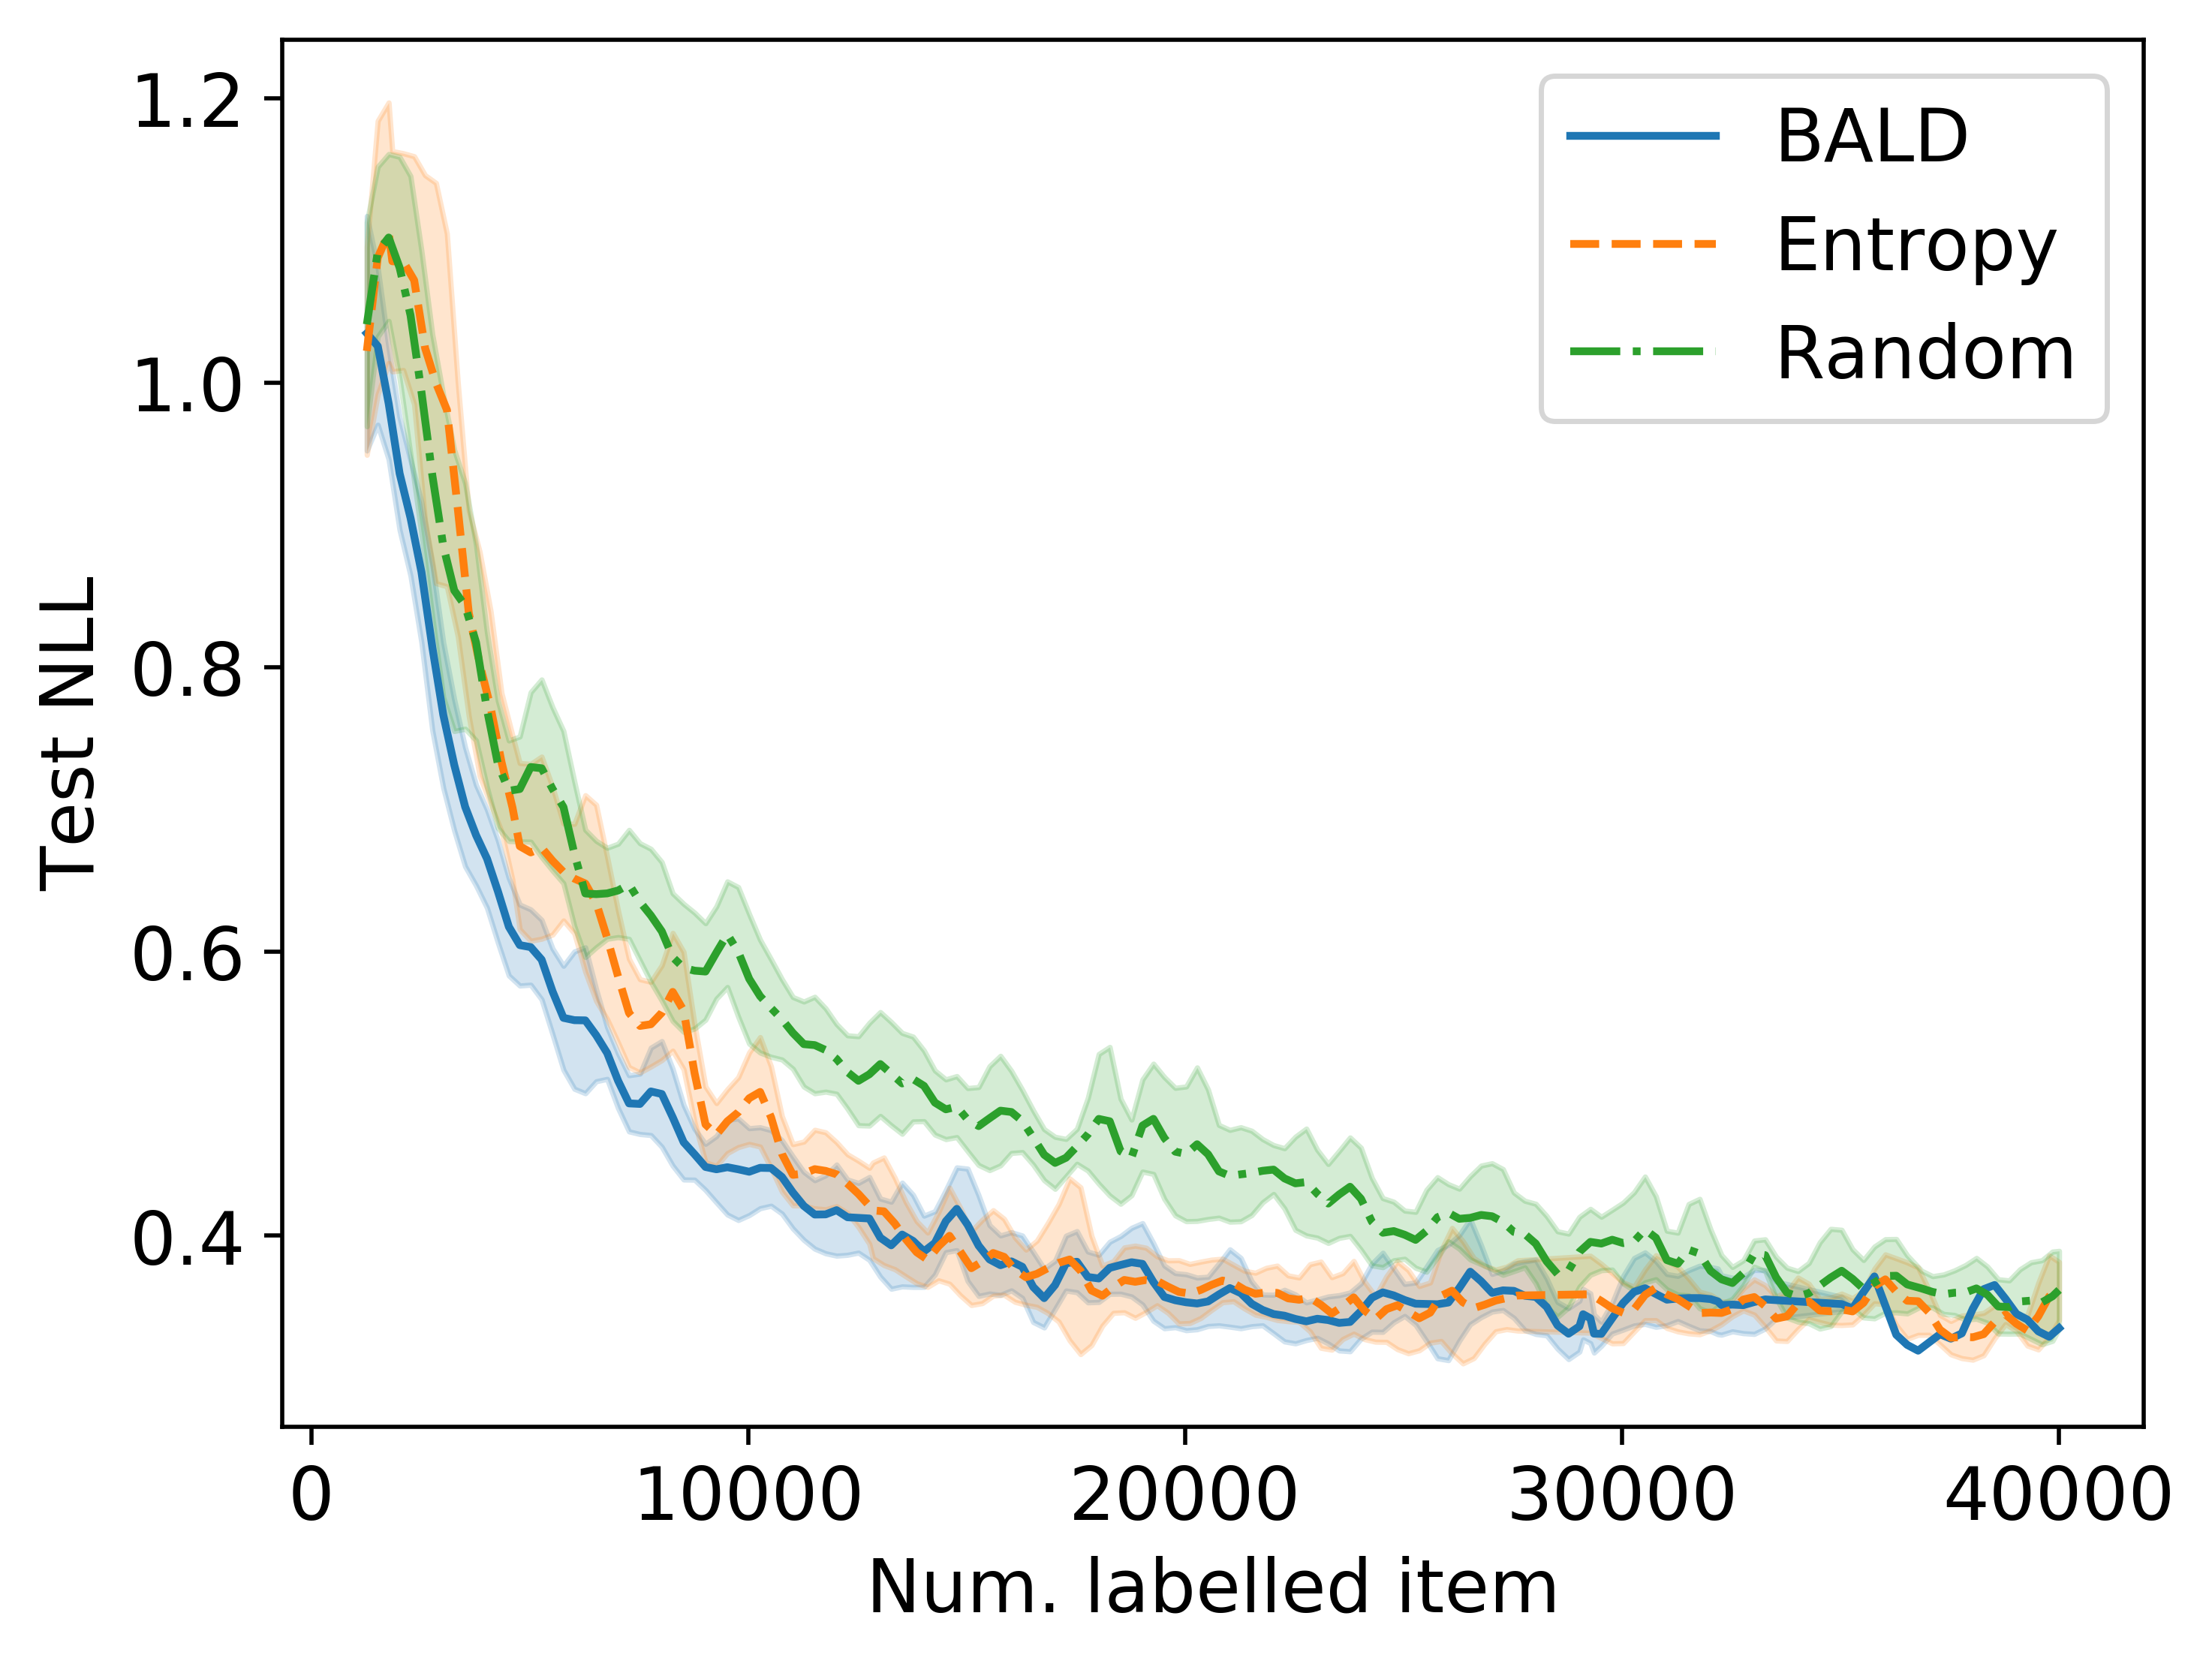
\includegraphics[width=0.4\textwidth]{fig/standard.png}
    \caption{Baselines results on CIFAR10 using MC-Dropout and VGG-16. On an academic dataset, both active learning techniques are competitive.}
    \label{fig:standard}
\end{figure}

\begin{abstract}
\vspace{-0.60cm}
   Active learning is able to reduce the amount of labelling effort by using a machine learning model to query the user for specific inputs.
   While there are many papers on new active learning techniques, these techniques rarely satisfy the constraints of a real-world project. In this paper, we analyse the main drawbacks of current active learning techniques and we present approaches to alleviate them. We do a systematic study on the effects of the most common issues of real-world datasets on the deep active learning process: model convergence, annotation error, and dataset imbalance. We derive two techniques that can speed up the active learning loop such as partial uncertainty sampling and larger query size. Finally, we present our open-source Bayesian active learning library, BaaL.
\end{abstract}

\bibliography{example_paper}
\bibliographystyle{icml2020}
% For submission, needs to be 2 documents and then concat together.
\end{document}



% This document was modified from the file originally made available by
% Pat Langley and Andrea Danyluk for ICML-2K. This version was created
% by Iain Murray in 2018, and modified by Alexandre Bouchard in
% 2019 and 2020. Previous contributors include Dan Roy, Lise Getoor and Tobias
% Scheffer, which was slightly modified from the 2010 version by
% Thorsten Joachims & Johannes Fuernkranz, slightly modified from the
% 2009 version by Kiri Wagstaff and Sam Roweis's 2008 version, which is
% slightly modified from Prasad Tadepalli's 2007 version which is a
% lightly changed version of the previous year's version by Andrew
% Moore, which was in turn edited from those of Kristian Kersting and
% Codrina Lauth. Alex Smola contributed to the algorithmic style files.

%%%%%%%% ICML 2020 EXAMPLE LATEX SUBMISSION FILE %%%%%%%%%%%%%%%%%

\documentclass{article}
\usepackage{times}
\usepackage{epsfig}
\usepackage{graphicx}
\usepackage{amsmath}
\usepackage{amssymb}
\usepackage{times}
\usepackage{epsfig}
\usepackage{graphicx}
\usepackage{amsmath}
\usepackage{amssymb}
% Include other packages here, before hyperref.
\usepackage{xcolor}
\usepackage[ruled,vlined,onelanguage]{algorithm2e}
\usepackage{setspace}
\usepackage{collcell}
\usepackage{xr}
\usepackage{natbib}
\usepackage{multirow}
\usepackage{subcaption}
\usepackage{mathtools}
\usepackage{colortbl,dcolumn}
\usepackage{algorithm2e}

% Include other packages here, before hyperref.

% If you comment hyperref and then uncomment it, you should delete
% egpaper.aux before re-running latex.  (Or just hit 'q' on the first latex
% run, let it finish, and you should be clear).
\usepackage[pagebackref=true,breaklinks=true,letterpaper=true,colorlinks,bookmarks=false]{hyperref}

% \cvprfinalcopy % *** Uncomment this line for the final submission

\def\cvprPaperID{****} % *** Enter the CVPR Paper ID here
\def\httilde{\mbox{\tt\raisebox{-.5ex}{\symbol{126}}}}

\newcommand{\todo}[1]{{\color{blue}TODO #1}}
\newcommand{\toref}[1]{{\color{red}REF #1 }}
\newcommand{\registered}{\textsuperscript{\tiny\textregistered}}
%\newcommand{\etal}{\textit{et al.}}
\renewcommand{\eqref}[1]{\hyperref[#1]{Eq.\ \ref*{#1}}}
\newcommand{\figref}[1]{\hyperref[#1]{Fig.\ \ref*{#1}}}
\newcommand{\tabref}[1]{\hyperref[#1]{Table\ \ref*{#1}}}
\newcommand{\secref}[1]{\hyperref[#1]{Section\ \ref*{#1}}}
\newcommand{\algoref}[1]{\hyperref[#1]{Algorithm\ \ref*{#1}}}
\newcolumntype{C}[1]{>{\centering}m{#1}}
\newcommand{\N}{{\cal N}}
\newcommand{\std}[1]{ \normalfont \color{darkgray}\footnotesize{$\pm$#1} }

% SYMBOL
\newcommand{\E}{{\mathbb E}}

\hypersetup{
    colorlinks=true,
    linkcolor=blue,
    filecolor=magenta,      
    urlcolor=blue,
}

\urlstyle{same}

% Recommended, but optional, packages for figures and better typesetting:
\usepackage{microtype}
\usepackage{booktabs} % for professional tables

% hyperref makes hyperlinks in the resulting PDF.
% If your build breaks (sometimes temporarily if a hyperlink spans a page)
% please comment out the following usepackage line and replace
% \usepackage{icml2020} with \usepackage[nohyperref]{icml2020} above.
\usepackage{hyperref}

% Attempt to make hyperref and algorithmic work together better:
\newcommand{\theHalgorithm}{\arabic{algorithm}}

% Use the following line for the initial blind version submitted for review:
%\usepackage{icml2020}

% If accepted, instead use the following line for the camera-ready submission:
\usepackage[accepted]{icml2020}

% The \icmltitle you define below is probably too long as a header.
% Therefore, a short form for the running title is supplied here:
\icmltitlerunning{Bayesian active learning for production. Supplementary Material}

\begin{document}

\twocolumn[
\icmltitle{Supplementary Material}]

\section{Implementation details}
Our methodology is as follows. We train a VGG-16 \citep{zhang2015accelerating} pretrained on ImageNet~\citep{imagenet_cvpr09}. Our initial training set contains 500 samples. We estimate the uncertainty using 20 MC samples and label the 100 most uncertain elements. Following \citet{gal2017deep}, we reset the weights to their initial value between steps. 

\section{Imbalanced datasets}
 
How to deal with imbalanced datasets is an entire area of research \citep{krawczyk2016learning}, but little has been done to deal with it when we are not aware of the \textit{a priori} class distribution. In consequence, the active learning model may quickly overfit to the more popular classes and reduce the effectiveness of active learning procedure. From \citet{gal2017deep}, it is known that Bayesian active learning will favor underrepresented classes. But, we find the reported experiments to be too simple. We  test this hypothesis in a controlled environment where we can set the number of unrepresented classes. 

In \tabref{fig:imbalanced}, we took the standard CIFAR100 dataset and we mimic an imbalanced dataset where few classes have a high number of examples. A class selected to be underrepresented sees its number of samples to be reduced by 75\%. When we increase the number of underrepresented classes, the gain of using MC-Dropout versus random sampling becomes more obvious. This is due to regions on the learned manifold associated with underrepresented classes to be highly uncertain. In consequence, these regions will be selected for labelling very early in the process.

% In this section, we investigated how common issues in deep learning are affecting active learning. While BALD is robust to data imbalance, it is highly affected by the annotation error or being under fitted.


\begin{table}
    \centering
    \begin{tabular}{llll}
    
    \toprule
    Dataset size &         5000 &        10000 &        20000 \\
    
    \hline
   $\Delta =10$ \\
    BALD &  4.39 \std{0.4} &  3.99 \std{0.01} &  3.57 \std{0.05} \\
    Entropy &  4.71 \std{0.02} &  4.54 \std{0.07} &  3.94 \std{0.01} \\
    Random &  4.52 \std{0.09} &  4.10 \std{0.03} &  3.71 \std{0.05} \\
    \hline
   $\Delta =25$ \\
    BALD &  4.40 \std{0.03}	&4.04\std{0.03} &	3.61\std{0.08} \\
    Entropy &  4.76 \std{0.02} &  4.68 \std{0.08} &   4.00 \std{0.01} \\
    Random &  4.58 \std{0.08} &  4.18 \std{0.04} &  3.75 \std{0.01} \\
    \hline 
   $\Delta =50$ \\
    BALD &  4.49 \std{0.08} &   4.07 \std{0.02} &   3.66 \std{0.04} \\
    Entropy &  4.83 \std{0.04} &  4.60 \std{0.14} &  4.07 \std{0.28} \\
    Random &  4.62 \std{0.03} &   4.21 \std{0.02} &   3.76 \std{0.04} \\
    \end{tabular}
    \caption{Effect of using active learning on imbalanced versions of CIFAR100. $\Delta$ is the number of class that contains 25\% of their data. From \citep{gal2017deep}, we know that BALD is robust to imbalanced datasets, but the study was not extensive. While BALD is robust to imbalanced datasets, the effect is catastrophic when using Entropy.  Performance averaged over 5 runs.}
    \label{fig:imbalanced}
\end{table}

\section{Effect of convergence}

In \figref{fig:active_gain}, we computed the difference in performance between BALD and random. We call this measure the \textit{Active gain} $= NLL_{Random} - NLL_{BALD}$. When using an underfitted model, the gain goes negative i.e. you would be better to use random selection.

\begin{figure}
    \centering
    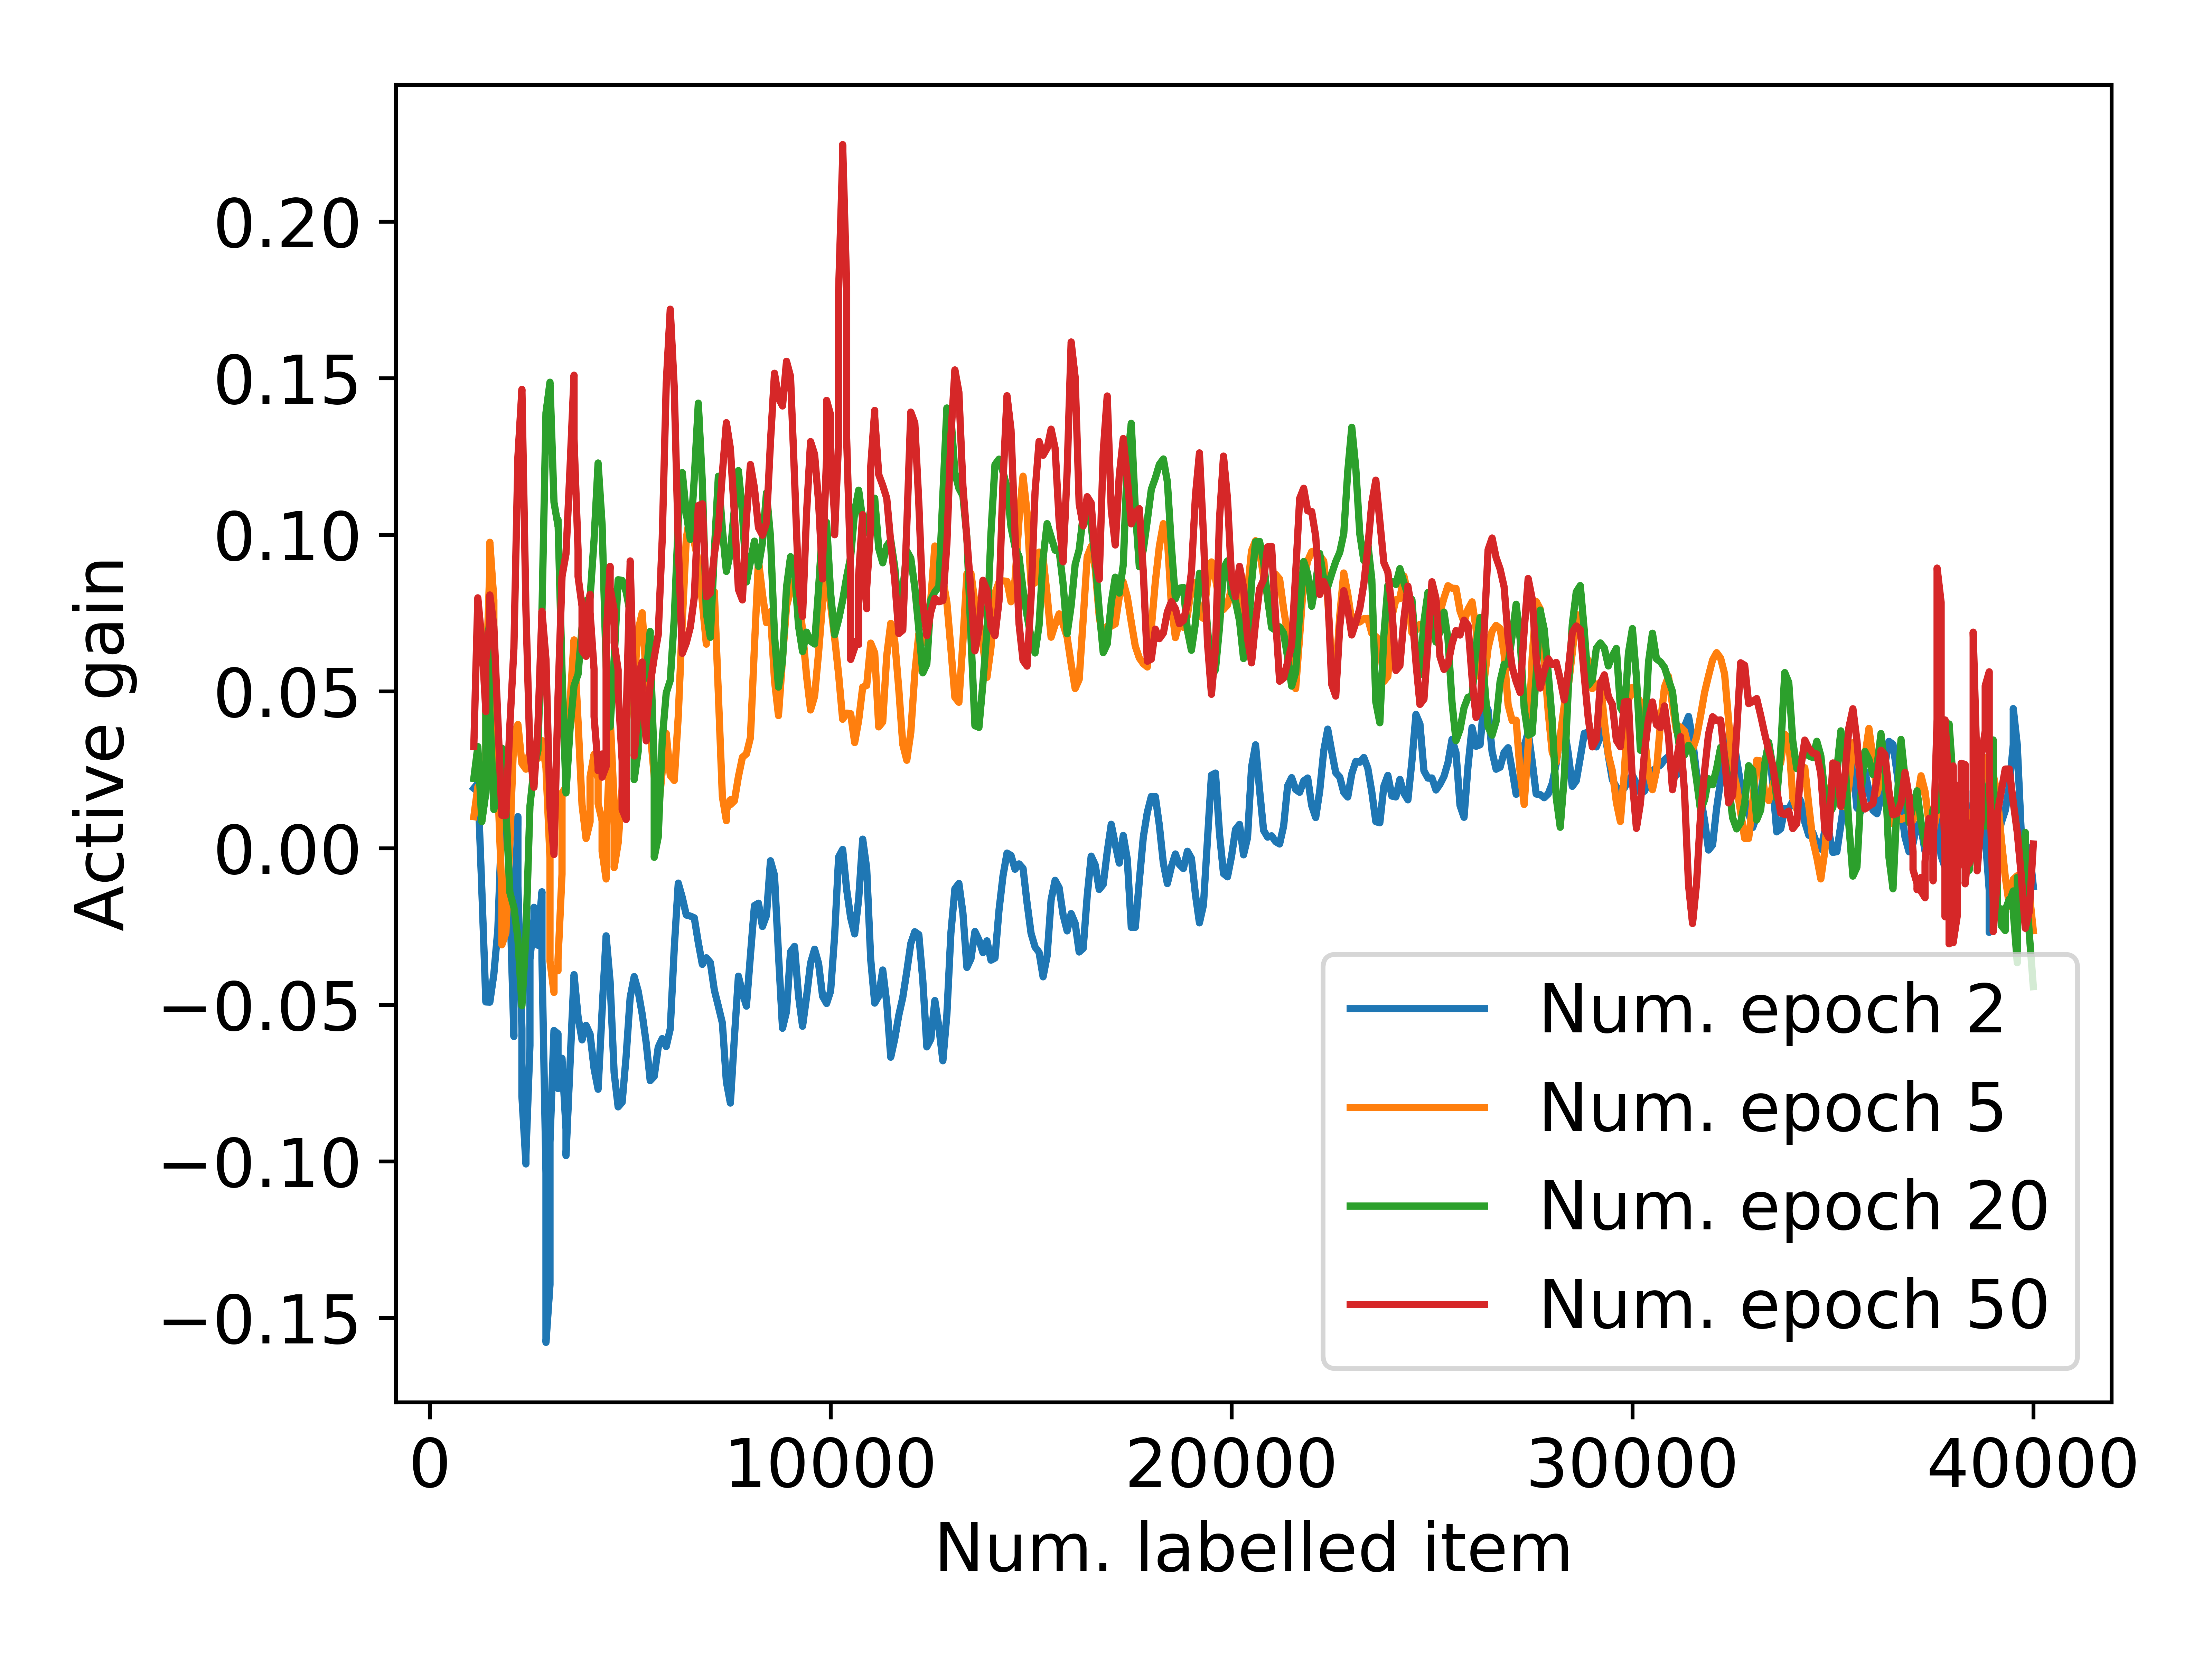
\includegraphics[width=0.5\textwidth]{fig/active_gain.png}
    \caption{Gain of using active learning when varying the number of training epochs. An underfitted model will cause harm to the model training and in this case, just using random would've been better.}
    \label{fig:active_gain}
\end{figure}

\section{Effect of reducing the pool size}
As part of the experiments, we test whether limiting the pool size would affect the performance of active learning. Our experiments in  \figref{fig:pool_size} show that whether to calculate the uncertainty for the whole pool data or a randomly selected subset, the performance of active learning is not affected. This leads to an the interesting outcome of limiting the uncertainty calculations (which is the most expensive part of an active learning loop) in production setup for faster active learning loops.

\begin{figure}
    \centering
    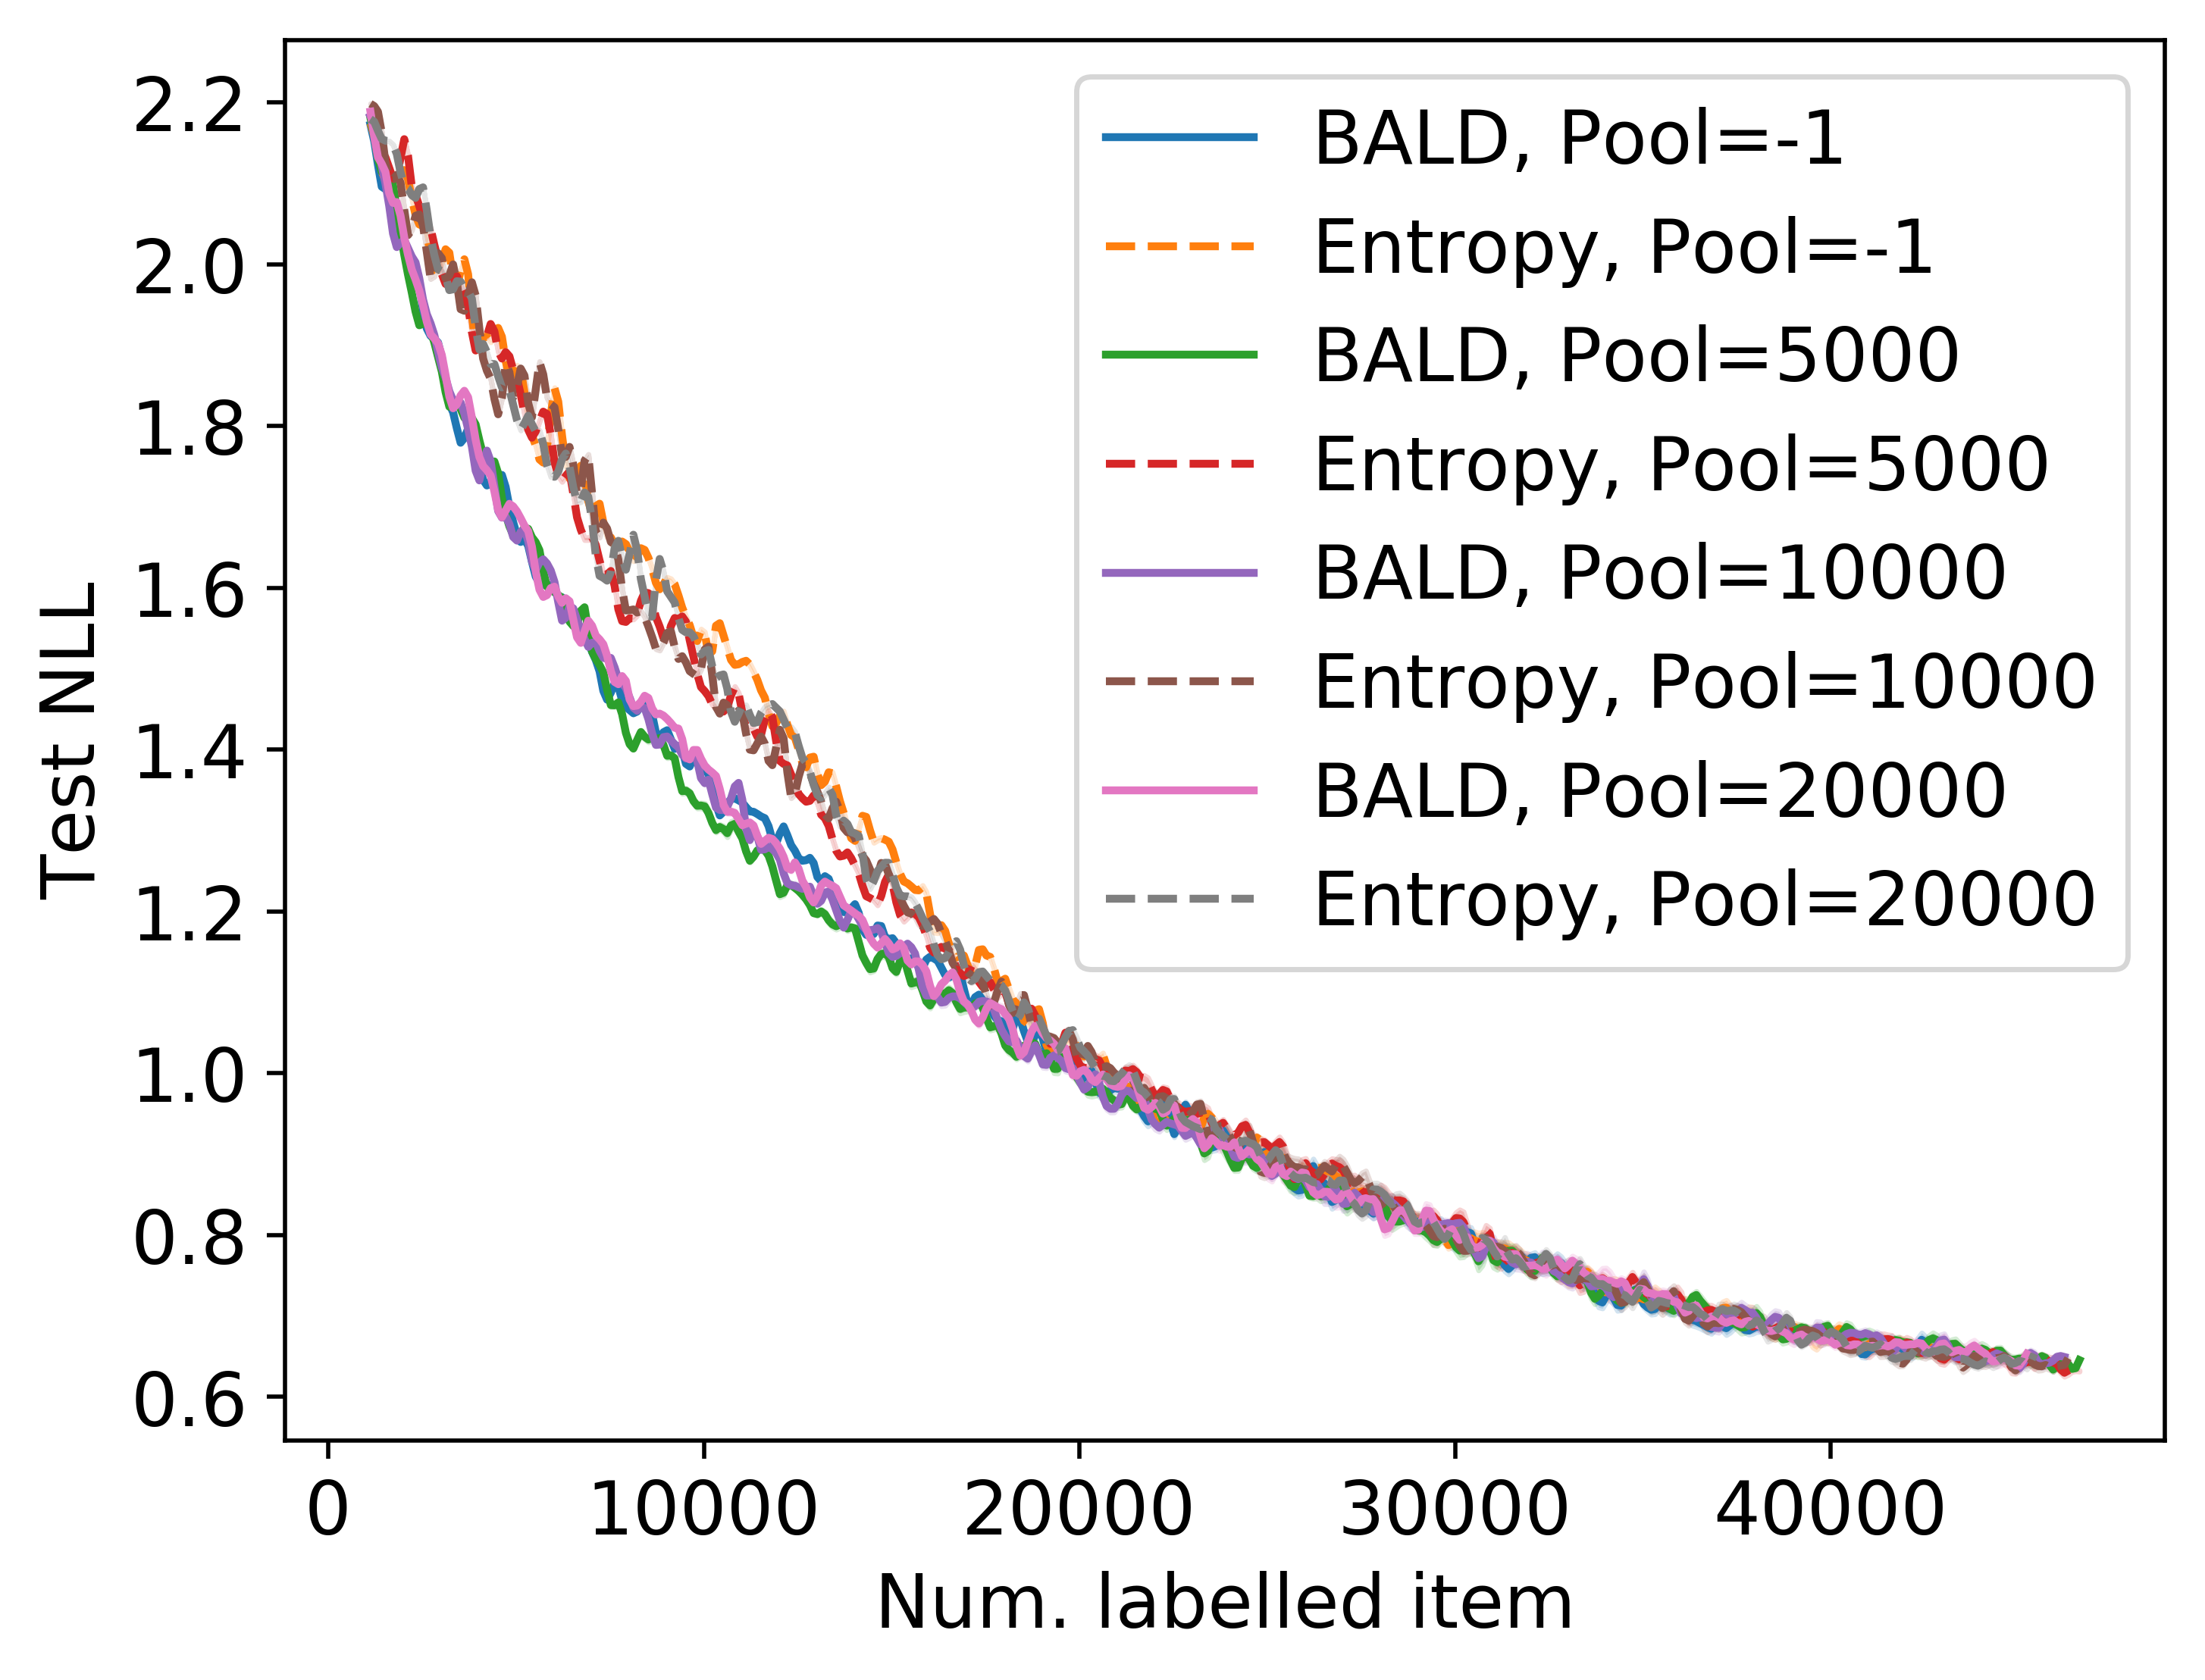
\includegraphics[width=0.4\textwidth]{fig/pol_size.png}
    \caption{Effect of reducing the size of the pool on CIFAR100. \textbf{-1} indicates no reduction. For all heuristics, the performance is not affected by the size of the pool showing that AL can be efficient when tuned properly.  Performance averaged over 5 runs.}
    \label{fig:pool_size}
\end{figure}

\begin{figure}
    \centering
    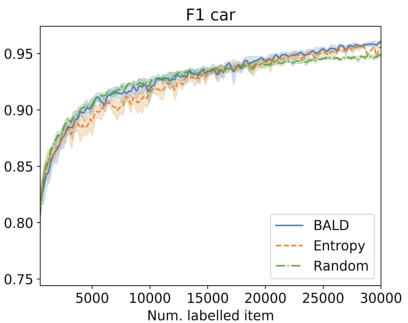
\includegraphics{fig/F1_Mio_tcd_annex.pdf}
    \caption{\textbf{F1 for the class \textit{car}}. BALD is great for underrepresented classes while not affecting more popular classes. Entropy decreases the performance on this class.}
    \label{fig:miotcd}
\end{figure}


\section{Bayesian active learning Library (BaaL)}

All the experiments in this paper have done using our publicly available Bayesian active learning library.  The goal of this library is to provide an easy to use but complete setup to test active learning on any project with few lines of code. We included features that current active learning libraries do not support. In particular, Bayesian methods such as MC-Dropout or Coresets are not widely available and there is no standard implementation of the active learning loop. Furthermore, research codebases are often hard to read and hard to maintain. Our proposed unified API could satisfy both research and industrial users.

 Our recently published open-source package named BaaL, aims at accelerating the transition from research to production. The core philosophy behind our library is to provide researchers with a well-designed API so that they focus on their novel idea and not on technical details. Our library proposes a task-agnostic system where one can mix-and-match any set of acquisition functions and uncertainty estimation methods.
The library consists of three main components:
\begin{enumerate}
    \item Dataset management to keep track and manage the labelled data $D_L$ and the unlabelled data $D_U$.
    \item Bayesian Methods i.e. MC-Dropout, MC-DropConnect and so on.
    \item Acquisition functions i.e. BALD, BatchBALD, Entropy and more.
\end{enumerate}

We provide full support for Pytorch \cite{paszke2017automatic} deep learning modules but our acquisition functions which are the most important part of active learning is implemented in  Numpy\cite{oliphant2006guide} and hence can be used on any platform. Our Data management module keeps track of what is labelled and what is unlabelled. We also provide facilitator methods to label a data point, update the pool of unlabelled data, and to randomly label a portion of the dataset. In our Bayesian module, we provide utilities to make any Pytorch model Bayesian with a single instruction. We also provide training, testing, and active learning loops that facilitate the active training procedure. Our acquisition functions are up-to-date with state-of-the-art methods. We provide easy to follow tutorials (https://baal.readthedocs.io/en/latest/) for each section of the library so that the user understands how each component works. Finally, our library is a member of Pytorch Ecosystem, which is reserved for libraries with outstanding documentation.

Our road-map has been indicated in the repository. Our current focus will include model calibration and semi-supervised learning. As more researchers contribute their methods to our library, we aim to become the standard Bayesian active learning library.

\end{document}
%%%%%%%% ICML 2020 EXAMPLE LATEX SUBMISSION FILE %%%%%%%%%%%%%%%%%

\documentclass{article}
\usepackage{times}
\usepackage{epsfig}
\usepackage{graphicx}
\usepackage{amsmath}
\usepackage{amssymb}
\usepackage{times}
\usepackage{epsfig}
\usepackage{graphicx}
\usepackage{amsmath}
\usepackage{amssymb}
% Include other packages here, before hyperref.
\usepackage{xcolor}
\usepackage[ruled,vlined,onelanguage]{algorithm2e}
\usepackage{setspace}
\usepackage{collcell}
\usepackage{xr}
\usepackage{natbib}
\usepackage{multirow}
\usepackage{subcaption}
\usepackage{mathtools}
\usepackage{colortbl,dcolumn}
\usepackage{algorithm2e}
\usepackage{standalone}

% Include other packages here, before hyperref.

% If you comment hyperref and then uncomment it, you should delete
% egpaper.aux before re-running latex.  (Or just hit 'q' on the first latex
% run, let it finish, and you should be clear).
\usepackage[pagebackref=true,breaklinks=true,letterpaper=true,colorlinks,bookmarks=false]{hyperref}

% \cvprfinalcopy % *** Uncomment this line for the final submission

\def\cvprPaperID{****} % *** Enter the CVPR Paper ID here
\def\httilde{\mbox{\tt\raisebox{-.5ex}{\symbol{126}}}}

\newcommand{\todo}[1]{{\color{blue}TODO #1}}
\newcommand{\toref}[1]{{\color{red}REF #1 }}
\newcommand{\registered}{\textsuperscript{\tiny\textregistered}}
%\newcommand{\etal}{\textit{et al.}}
\renewcommand{\eqref}[1]{\hyperref[#1]{Eq.\ \ref*{#1}}}
\newcommand{\figref}[1]{\hyperref[#1]{Fig.\ \ref*{#1}}}
\newcommand{\tabref}[1]{\hyperref[#1]{Table\ \ref*{#1}}}
\newcommand{\secref}[1]{\hyperref[#1]{Section\ \ref*{#1}}}
\newcommand{\algoref}[1]{\hyperref[#1]{Algorithm\ \ref*{#1}}}
\newcolumntype{C}[1]{>{\centering}m{#1}}
\newcommand{\N}{{\cal N}}
\newcommand{\std}[1]{ \normalfont \color{darkgray}\footnotesize{$\pm$#1} }

% SYMBOL
\newcommand{\E}{{\mathbb E}}
\newcommand{\Q}{{\mathbb Q}}

\hypersetup{
    colorlinks=true,
    linkcolor=blue,
    filecolor=magenta,      
    urlcolor=blue,
}

\urlstyle{same}

% Recommended, but optional, packages for figures and better typesetting:
\usepackage{microtype}
\usepackage{booktabs} % for professional tables
\setlength{\abovedisplayskip}{-2pt}
\setlength{\belowdisplayskip}{-2pt}

% hyperref makes hyperlinks in the resulting PDF.
% If your build breaks (sometimes temporarily if a hyperlink spans a page)
% please comment out the following usepackage line and replace
% \usepackage{icml2020} with \usepackage[nohyperref]{icml2020} above.
\usepackage{hyperref}

% Attempt to make hyperref and algorithmic work together better:
\newcommand{\theHalgorithm}{\arabic{algorithm}}

% Use the following line for the initial blind version submitted for review:
%\usepackage{icml2020}

% If accepted, instead use the following line for the camera-ready submission:
\usepackage[accepted]{icml2020}

% The \icmltitle you define below is probably too long as a header.
% Therefore, a short form for the running title is supplied here:
\icmltitlerunning{Bayesian active learning for production}
\begin{document}

\twocolumn[
\icmltitle{Bayesian active learning for production, a systematic study and a reusable library}

% It is OKAY to include author information, even for blind
% submissions: the style file will automatically remove it for you
% unless you've provided the [accepted] option to the icml2020
% package.

% List of affiliations: The first argument should be a (short)
% identifier you will use later to specify author affiliations
% Academic affiliations should list Department, University, City, Region, Country
% Industry affiliations should list Company, City, Region, Country

% You can specify symbols, otherwise they are numbered in order.
% Ideally, you should not use this facility. Affiliations will be numbered
% in order of appearance and this is the preferred way.
\icmlsetsymbol{equal}{*}

\begin{icmlauthorlist}
\icmlauthor{Parmida Atighehchian}{equal,eai}
\icmlauthor{Fr\'ed\'eric Branchaud-Charron}{equal,eai}
\icmlauthor{Alexandre Lacoste}{eai}
\end{icmlauthorlist}

\icmlaffiliation{eai}{Element AI, Montr\'eal, Canada}

\icmlcorrespondingauthor{Fr\'ed\'eric Branchaud-Charron}{frederic.branchaud-charron@elementai.com}

% You may provide any keywords that you
% find helpful for describing your paper; these are used to populate
% the "keywords" metadata in the PDF but will not be shown in the document
\icmlkeywords{Machine Learning, Active Learning, Uncertainty Estimation}

\vskip 0.3in
]

% this must go after the closing bracket ] following \twocolumn[ ...

% This command actually creates the footnote in the first column
% listing the affiliations and the copyright notice.
% The command takes one argument, which is text to display at the start of the footnote.
% The \icmlEqualContribution command is standard text for equal contribution.
% Remove it (just {}) if you do not need this facility.

%\printAffiliationsAndNotice{}  % leave blank if no need to mention equal contribution
\printAffiliationsAndNotice{\icmlEqualContribution} % otherwise use the standard text.

\begin{figure}
    \centering
    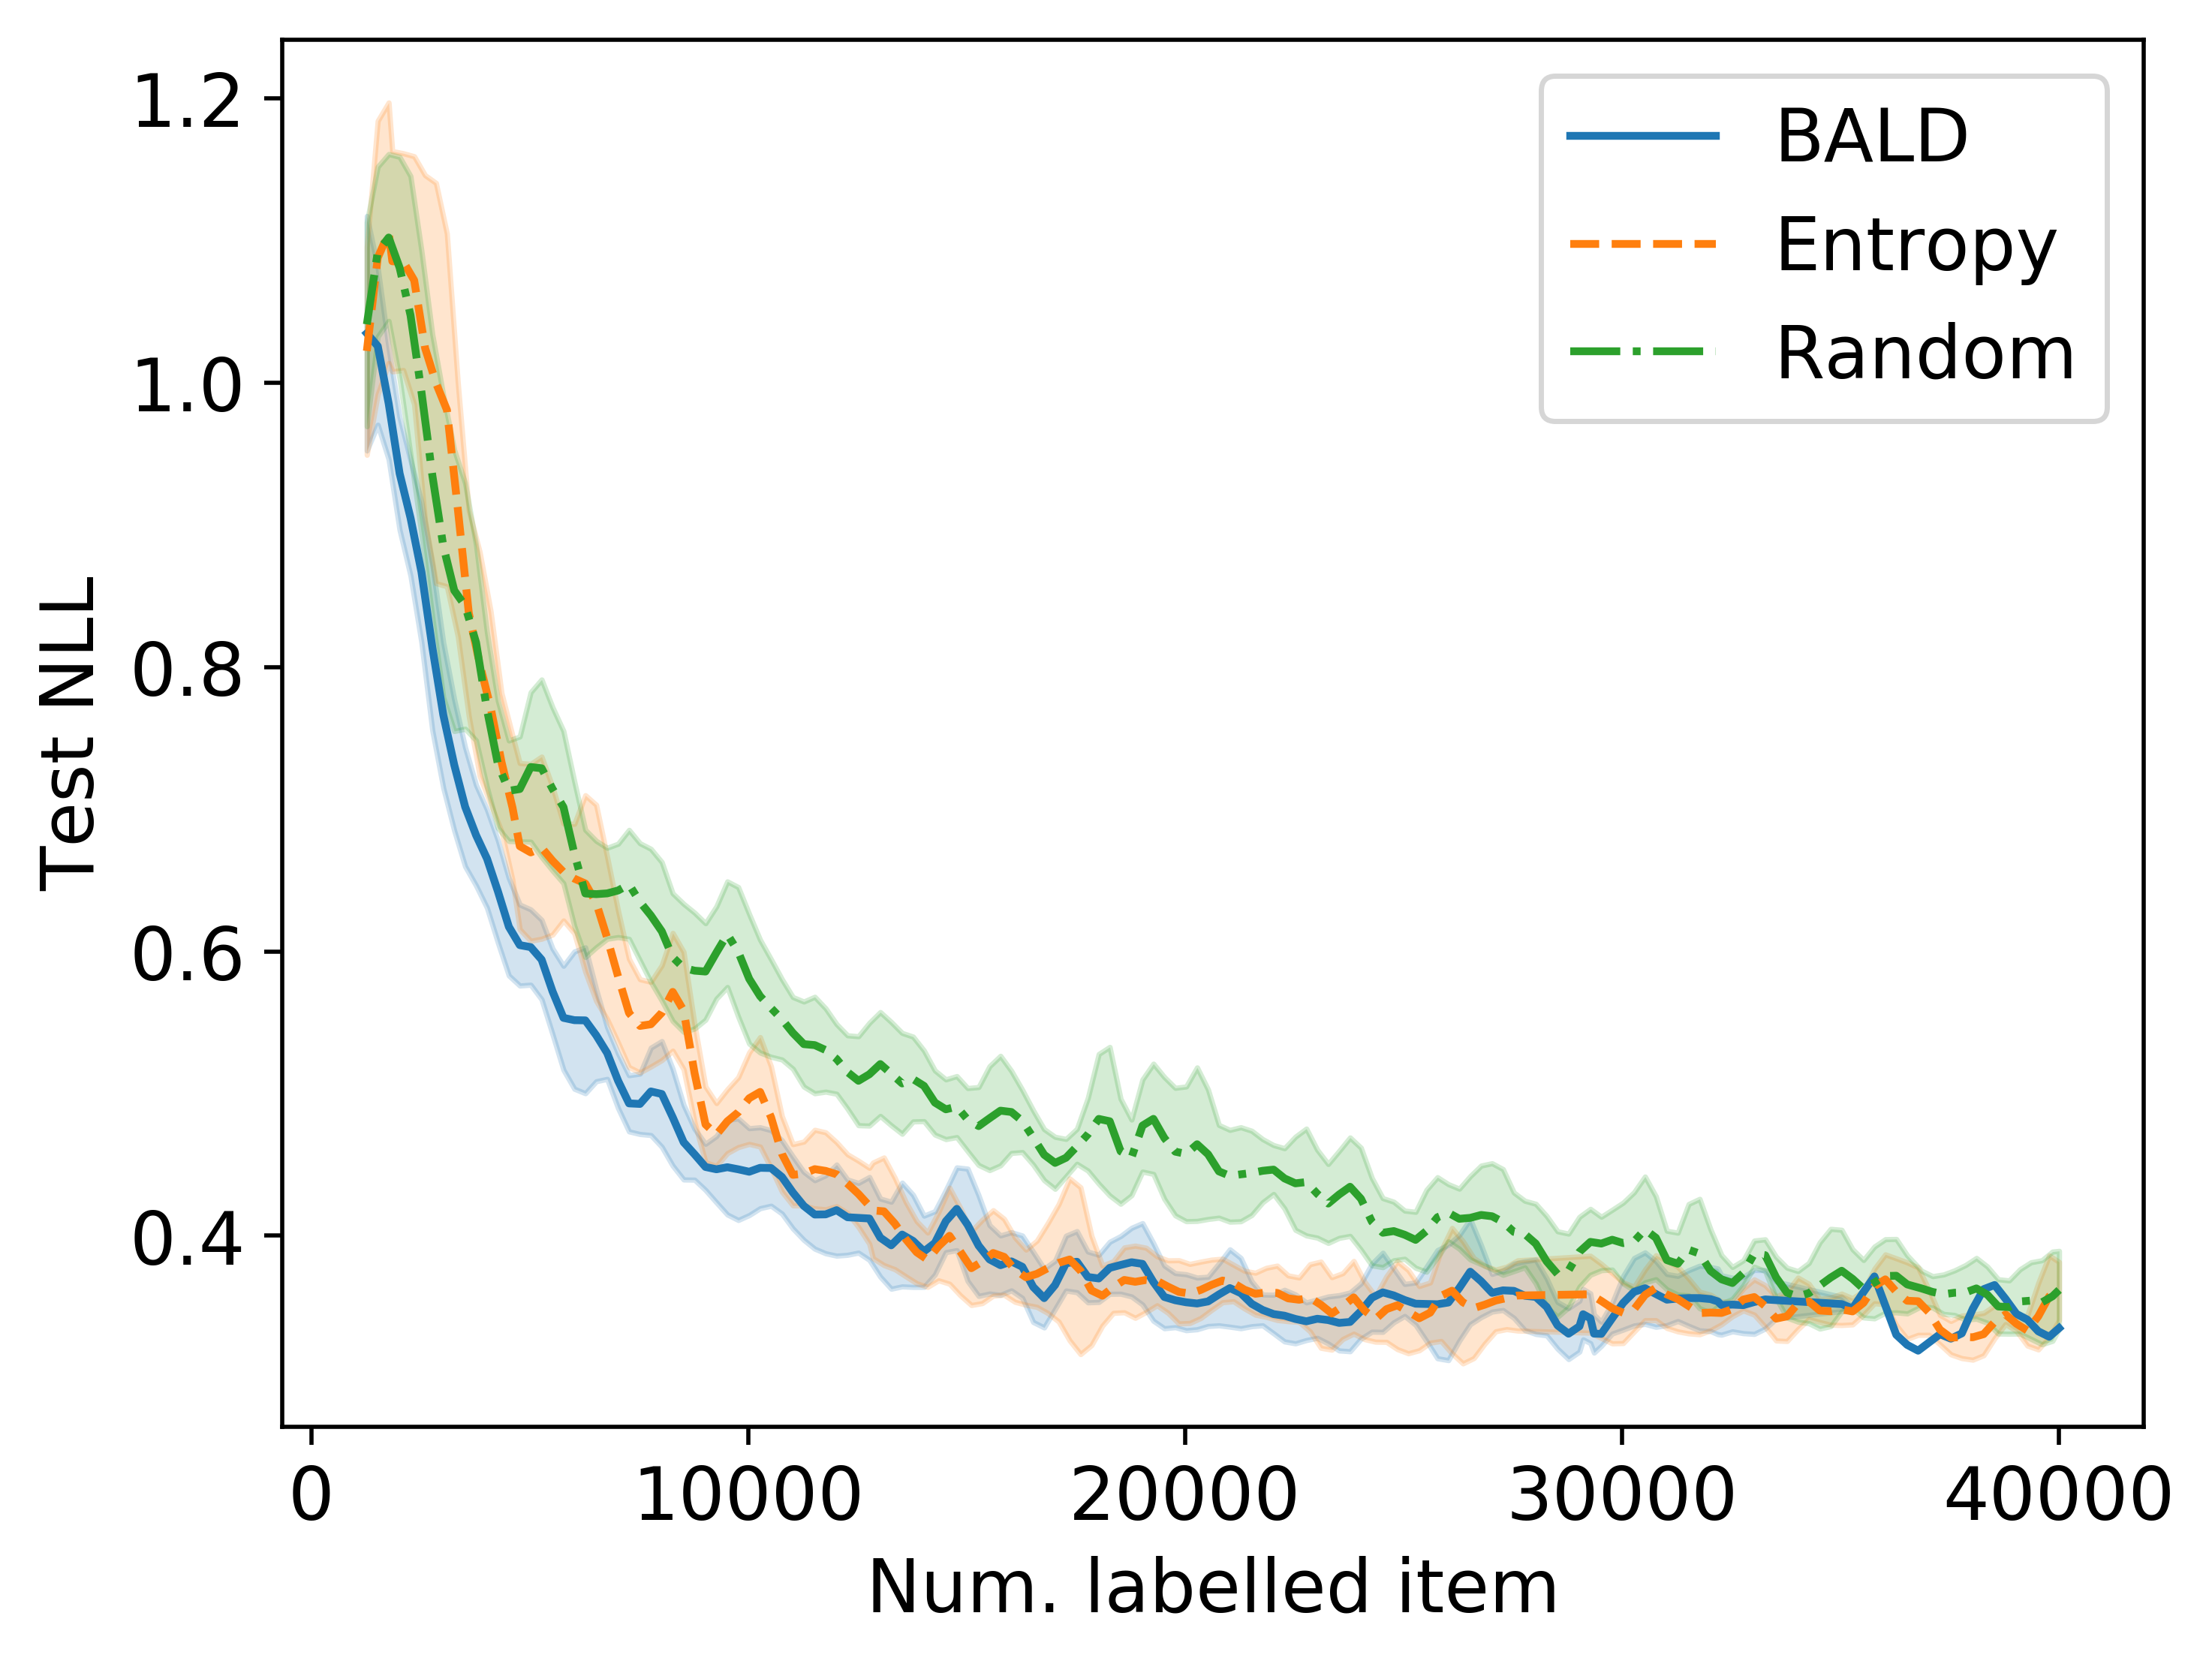
\includegraphics[width=0.4\textwidth]{fig/standard.png}
    \caption{Baselines results on CIFAR10 using MC-Dropout and VGG-16. On an academic dataset, both active learning techniques are competitive.}
    \label{fig:standard}
\end{figure}

\begin{abstract}
\vspace{-0.60cm}
   Active learning is able to reduce the amount of labelling effort by using a machine learning model to query the user for specific inputs.
   While there are many papers on new active learning techniques, these techniques rarely satisfy the constraints of a real-world project. In this paper, we analyse the main drawbacks of current active learning techniques and we present approaches to alleviate them. We do a systematic study on the effects of the most common issues of real-world datasets on the deep active learning process: model convergence, annotation error, and dataset imbalance. We derive two techniques that can speed up the active learning loop such as partial uncertainty sampling and larger query size. Finally, we present our open-source Bayesian active learning library, BaaL.
\end{abstract}

%%%%%%%%% BODY TEXT

%%%%%%%%%%%%%%%%%%%%%%%%%%%
%% See https://docs.google.com/document/d/148Rkq9R44TIT4QdDR8jsHhQ3zBIPdbVbrjEFkod4hV8/edit?usp=sharing
%%%%%%%%%%%%%%%%%%%%%%%%%%%%
\section{Introduction}
The amount of data readily available for machine learning has exploded in recent years. 
However, for data to be used for deep learning models, labelling is often a required step. 
A common problem when labelling new datasets is the required human effort to perform the annotation. In particular, tasks that require particular domain knowledge such as medical imaging, are expensive to annotate. To solve this, active learning (AL) has been proposed to only label the core set of observations useful for training.

While the active learning field includes many approaches \citep{kirsch2019batchbald, tsymbalov2019deeper, beluch2018power, maddox2019simple}, these methods are often not scalable to large datasets or too slow to be used in a more realistic environment e.g. in a production setup. In particular, active learning applied to images or text requires the usage of deep learning models which are slow to train and themselves require a noticeable huge amount of data to be effective \citep{imagenet_cvpr09, abu2016youtube}.

Furthermore, deep learning models require carefully tuned hyperparameters to be effective. In a research environment, one can fine-tune and perform hyperparameter search to find the optimal combination that gives the biggest reduction in labelling  effort. In a real-world setting, the hyperparameters are set at the beginning with no guarantee for the outcome.

Finally, in a real-world setup, the data is often not cleaned nor balanced. In particular, studies have shown that humans are far from perfect when labelling and the problem is even worse when using crowd-sourcing \citep{ipeirotis2010quality, allahbakhsh2013quality}.

Our contributions are three-fold. We perform a systematic study on the effect of the most common pathologies found in real-world datasets on active learning. Second, we propose several techniques that make active learning suitable for production. Finally, we present a case study of using active learning on a real-world dataset. 

In addition, we present our freely available Bayesian active learning library, BaaL\footnote{\url{https://github.com/ElementAI/baal}} which provides all the necessary set up and tools for active learning experiments at any scale.

\section{Problem setting}

We consider the problem of supervised learning where we observe a dataset made of $n$ pairs $D_L= \{(x_i, y_i)\}_i^{N}$ and our goal is to estimate a prediction function $p(y\mid x)$. In addition, we have $N'$ observations without label $D_U = \{x_i\}_i^{N'}$. More specifically, we consider the problem of active learning where the algorithm is summarized in \algoref{algo:al}.

\begin{algorithm}
 \KwData{$D = \{x_0, \ldots, x_n\}$}
 \KwResult{$D_L = \{(x_0, y_0), \ldots\}$}
 ~~$D_L \leftarrow$ Label randomly B points\;\\
 $D_U \leftarrow D \setminus D_L$ \;\\
\While{labelling budget is available}{
  Train model to convergence on $D_L$\;\\
  Compute uncertainty $U(x), \text{for all } x \in D_U$\;\\
  Label top-\textit{k} most uncertain samples\;
 }
 \caption{\textbf{Active learning process.} For batch active learning, the algorithm train a model on $D_L$ before estimating the uncertainty on the pool $D_U$, the most uncertain samples are labelled by a human before restarting the loop.}
 \label{algo:al}
\end{algorithm}

%-------------------------------------------------------------------------
\section{Background}\label{background}
%The goal of active learning is to reduce the labelling effort without giving up on model performance. Deep Learning models are powerful solutions given a good representation of the domain \citep{krizhevsky2012imagenet, ioffe2015batch}. Unfortunately, acquiring and labelling  data is a tedious, time-consuming and expensive task. Reducing the number of samples we need to label is key to make deep learning more affordable.
% ICML CUT In the past years, there have been different attempts of adjusting active learning for deep learning models. The most complete literature for active learning is concentrated on
Active learning has received a lot of attention in the past years, specifically on classification tasks \citep{gal2017deep}. However, some work has been done on segmentation \citep{kendall2017uncertainties}, localization \citep{miller2019evaluating}, natural language processing \citep{siddhant2018deep}, and time series \citep{peng2017acts}. In this paper, we focus our attention on image classification. %There are several challenges involved in changing the training procedure of a model to active training. 

\paragraph{Bayesian active Learning}
Current state-of-the-art techniques used in active learning relies on uncertainty estimation to perform queries~\citep{gal2017deep}.
%\todo{No evidence, needs at least a ref: For once, the more complicated the task, the harder to estimate the model uncertainty and hence, it is more challenging to achieve the state of the art model accuracy/precision with active learning.} 
%The  active learning procedure is time-consuming due to the need to retrain the model between queries. In a perfect scenario, one would imagine to have an active training framework in which the annotator could get new queries to be labelled as soon as possible, i.e. the model should be fast enough to compute the uncertainty between each sample labelled. 
A common issue highlighted in \citet{tsymbalov2019deeper, kirsch2019batchbald} is the need to retrain the model and recompute the uncertainties as often as possible. Otherwise, the next samples to be selected may be too similar to previously annotated samples. This is problematic due to the long training time of deep-learning models as well as the expensive task of uncertainty estimation.
\citet{tsymbalov2019deeper, houlsby2011bayesian} and \citet{Wilson2015DeepKL} proposed solutions to this issue, are memory expensive and time-consuming when used on large input size or large datasets.
In reality, due to the large cost of inference and retraining for large scale datasets, it is not feasible to recompute the uncertainties in a timely fashion. In consequence, multiple samples are annotated between retraining. We call this framework batch active learning.

%FRED: This needs to be moved
% The idea behind bayesian active learning is simple, the model is able to to actively “query” example(s) to be labelled. By doing that, we hope to label only the most effective samples for training the model instead of random selection. 
%CUT ICML There are, at a high level, two types of strategies for choosing data points for labelling . One is to sample data points you hope will be most representative of your dataset as a whole, in order for any model you train to quickly learn features that represent fundamental variation in the data. The other is to choose data points that will maximize the information gain from a model trained in parallel.
%CUT ICML Sampling data points at random is a naive example of the first strategy. It would sample from the data distribution which contains uninformative samples. However, there are ways to improve on this, for example by clustering the data and using this cluster structure to sample a diverse representative set of observation. \citet{sener2017active} are proposed as a way to extract a subset representative of the overall distribution of the dataset. In this paper, we will focus on the second strategy.
Machine leanings algorithms can suffer from two types of uncertainties \citep{kendall2017uncertainties}:

1) \emph{Aleatoric Uncertainty}, the uncertainty intrinsic to the data, which cannot be explained with more samples. This is due to e.g.: errors during labelling, occlusion, poor data acquisition ,or when two classes are highly confused. 

2) \emph{Epistemic Uncertainty}, the uncertainty about the underlying model. Obtaining more samples will provide more information about the underlying model and reduce the amount of epistemic uncertainty. Crucially, some samples are more informative than others. 

\paragraph{Uncertainty estimations} 
Computing the uncertainty of deep neural networks is crucial to many applications from medical imaging to loan application. Unfortunately, deep neural networks are often overconfident as they are not designed to provide calibrated predictions \citep{scalia2019evaluating,gal2016uncertainty}. Hence, researchers proposed new methods to get a trustful estimation of the epistemic uncertainty such as MC-Dropout \citep{gal2016dropout}, Bayesian neural networks \citep{blundell2015weight} or Ensembles. More recently, \citet{wilson2020bayesian} proposed to combine variational inference and ensembles. While this approach is state-of-the-art, it is far too computationally expensive to be used in the industry.

%In this paper, we will focus on MC-Dropout because it can be used with most common architectures and has a non-prohibitive inference time when optimally implemented.

In this paper, we will use MC-Dropout \citep{gal2016dropout}. In this technique proposes the Dropout layers are kept activated at test time to sample from the posterior distribution. Hence, this method can be used on any architecture that uses Dropout which makes it usable on a wide range of applications.

% Should we say that BNN estimates both aleactoric and epistemic while MCDropout + BALD just estimate epistemic (Gal et al.)

\paragraph{Acquisition functions}
Many heuristics have been proposed to extract the uncertainty value from the stochastic prediction sampling. We define  Monte-Carlo sampling from the posterior distribution $p(w\mid D)$ as:
\begin{equation*}
    p_t(y \mid x) = p(y \mid x, w_t), t \in \{1 \ldots T\}, w_t \sim p(w\mid D)
\end{equation*}

where $T$ is the number of Monte-Carlo samples. %For example, a classification task with $C$ classes, $p$ contains a matrix $C\times T$.
We compute the Bayesian model average, $\hat p(y \mid x) = \frac{1}{T} \sum_t^T p_t(y \mid x)$. When highly uncertain, $\hat p(y \mid x)$ will be close to a uniform distribution. A naive approach to estimate the uncertainty is to compute the entropy of this distribution.

% \begin{align*}
%     U(x) =& \sum_c \hat p(y = c \mid x) * \log(\hat p(y = c \mid x)).
% \end{align*}

% By assuming a Gaussian prior over the weights, we can compute 
% \begin{equation*}
%     U(X) = \E_c[Var(p(y=c \mid x))]
% \end{equation*}
% the expected variance of the model.

A more sophisticated approach is BALD~\citep{houlsby2011bayesian}, which estimates the epistemic uncertainty by computing the mutual information between the model posterior distribution and the prediction:
\begin{equation*}
    I(y, w \mid x, D_L) = H[y \mid x, D_L] - \E_{p(w \mid D_L)}(H[y \mid x, w]).
\end{equation*}


BALD compares the entropy of the mean estimator to the entropies of all estimators. The result is high when there are high disagreements between predictions, which addresses the overconfidence issue in deep learning models.

% We can combine this network with MC-Dropout such that the BALD uncertainty can be computed with:

% \begin{align*}
%     U(x) &= H[y \mid x, D_L] - \E_{p(w \mid D_L)}(H[y \mid x, w]) \\
%     &= H[y \mid x, D_L] - \frac{1}{T} \sum_t^T \sum_c^C f_c(x) \log f_c(x) \\
%     &= \hat f(x) \log \hat f(x) - \frac{1}{T} \sum_t^T \sum_c^C f_c(x) \log f_c(x). 
% \end{align*}

\section{Experiments}

In this paper, we want to demonstrate the usability of active learning in a real-world scenario. First, we analyze the effect of common pathologies in deep learning on active learning. Secondly, a common issue in active learning is the time required between steps in the active learning loop. As stated by \citet{kirsch2019batchbald}, retraining as soon as possible is crucial to obtain decorrelated samples. We investigate if a) this is the case in large-scale datasets and b) what can we do to make this faster. Implementation details can be found in Annex. Baselines for all  acquisition functions can be found in \figref{fig:standard}.

% Our methodology is as follow. We use a VGG-16 \citep{zhang2015accelerating} with an input size of $224 \times 224$. The inputs are preprocessed according to the standard preprocessing pipeline of ImageNet \citep{imagenet_cvpr09}. At each active learning step, we reset the network to its initial weights and train to convergence. We then predict on the unlabelled pool using 20 Monte-Carlo inferences. Finally, we label the 100 most uncertain elements and add them to $D_L$. For all experiments, we report the performance over 5 runs. Baselines for BALD, Entropy and Random acquisition functions can be found in \figref{fig:standard}. Beside the random baseline, BALD and Entropy are similar.





%CUT ICML We train the network on the current labelled dataset for 50 epochs using standard SGD optimizer with 0.001 learning rate, 0.9 momentum and $5e^-4$ weight decay. We then perform 20 Monte-Carlo inference passes on each unlabelled image and use the heuristic to rank samples from the most to the least informative. 
% FRED: Keep for later? To remove sampling bias\toref, we shuffle 5\% of the samples.
%CUT ICML Finally, we label the top $K$ elements and add them to $D_L$. The active learning procedure stops once we reach a plateau ie. the model is not improving anymore when we add new data.

\subsection{Pathologies}\label{pathologies}
In this section, we verify if common pathologies in deep learning hold for active learning. Problems such as annotation error or  model convergence % or imbalanced dataset (already covered in \citet{gal2017deep}, but we make a deeper study in Annex)
may be hurtful to the procedure and are often overlooked in the literature. In particular, due to the small amount of annotated data, models are more at risk than when they are trained on large datasets.


\paragraph{Effect of annotation error}
While standard datasets are of good quality, humans are far from perfect and will produce errors when labelling. This is especially true when using crowdsourcing \citep{allahbakhsh2013quality}.
Because active learning relies on the training data to train a model and there are only a few labelled samples, we make the hypothesis that active learning would be highly sensitive to noise.

To confirm this hypothesis, we introduce noise by corrupting $\lambda \%$ of the labels. We test our hypothesis on CIFAR10~\citep{krizhevsky2009learning}. In \tabref{fig:labl_noise}, we can assess that depending on $\lambda$, the active learning procedure is highly affected by labelling noise. Furthermore, when we compare to random selection, the gain of using active learning decreases when noise is involved, but it is still useful.% Furthermore, one could identify errors later in the procedure as \citet{brodley1999identifying} proposes.

\begin{table}
    \centering
    {\small
    \begin{tabular}{llll}
\toprule
Dataset size &            5000 &           10000 &           20000 \\
\midrule
     $\lambda$=               0 &                 &                 \\
     \hline
        BALD &  0.65 \std{0.01} &  0.53 \std{0.01} &  0.43 \std{0.02} \\
     Entropy &  0.68 \std{0.03} &  0.52 \std{0.02} &  0.43 \std{0.03} \\
      Random &  0.71 \std{0.02} &  0.58 \std{0.02} &  0.47 \std{0.01} \\
      \hline
     $\lambda$=            0.05 &                 &                 \\
     \hline
        BALD &  0.72 \std{0.02} &  0.57 \std{0.01} &  0.43 \std{0.02} \\
     Entropy &  0.72 \std{0.02} &  0.54 \std{0.02} &  0.41 \std{0.01} \\
      Random &  0.73 \std{0.03} &  0.61 \std{0.03} &  0.51 \std{0.02} \\
      \hline
     $\lambda$ =             0.1 &                 &                 \\
     \hline
        BALD &  0.78 \std{0.03} &  0.62 \std{0.01} &  0.48 \std{0.01} \\
     Entropy &  0.71 \std{0.02} &  0.57 \std{0.01} &  0.44 \std{0.02} \\
      Random &  0.76 \std{0.02} &  0.64 \std{0.02} &  0.54 \std{0.01} \\
\bottomrule
\end{tabular}}

    \caption{Effect of annotation error on active learning by randomly shuffling $\lambda$\% labels. The test log-likelihood is averaged over 5 runs.}
    %By randomly shuffling $\lambda$\% labels, we recreate a real-world situation. Active learning suffers greatly from this pathology and BALD even more so than Entropy. Performance averaged over 5 runs.}
    \label{fig:labl_noise}
\end{table}


\paragraph{Effect of model convergence}

Because we have no control over the training regime at each time step, it is hard to train the model to an optimal solution. With fully annotated datasets, we can fine-tune our training setup with hyper-parameter search or train for days at a time. In a production environment, we are limited in our ability to best train the model. % needs to be trained in a timely fashion. Moreover, we cannot select the best training setup, since it may change from step to step. 
In consequence, the model may be under or overfitted to the current dataset and provide flawed uncertainty estimations. %Finally, the size of the validation set is often quite small and may not be an accurate representation of the domain.

To confirm our hypothesis, we vary the number of epochs the model is trained for. As seen in \figref{fig:convergence}, underfitted models are highly affected while overfitted models suffer, but are still performant. This is due to a poor fit of the model that lead to a wrong estimation of the model uncertainty. %Note that this experiment is also a valid way to accelerate the active learning loop, but this hyperparameter would be hard to fine-tune in a real-world situation.
In Annex, we present the difference in performance between BALD and Random.

\begin{figure}
    \centering
    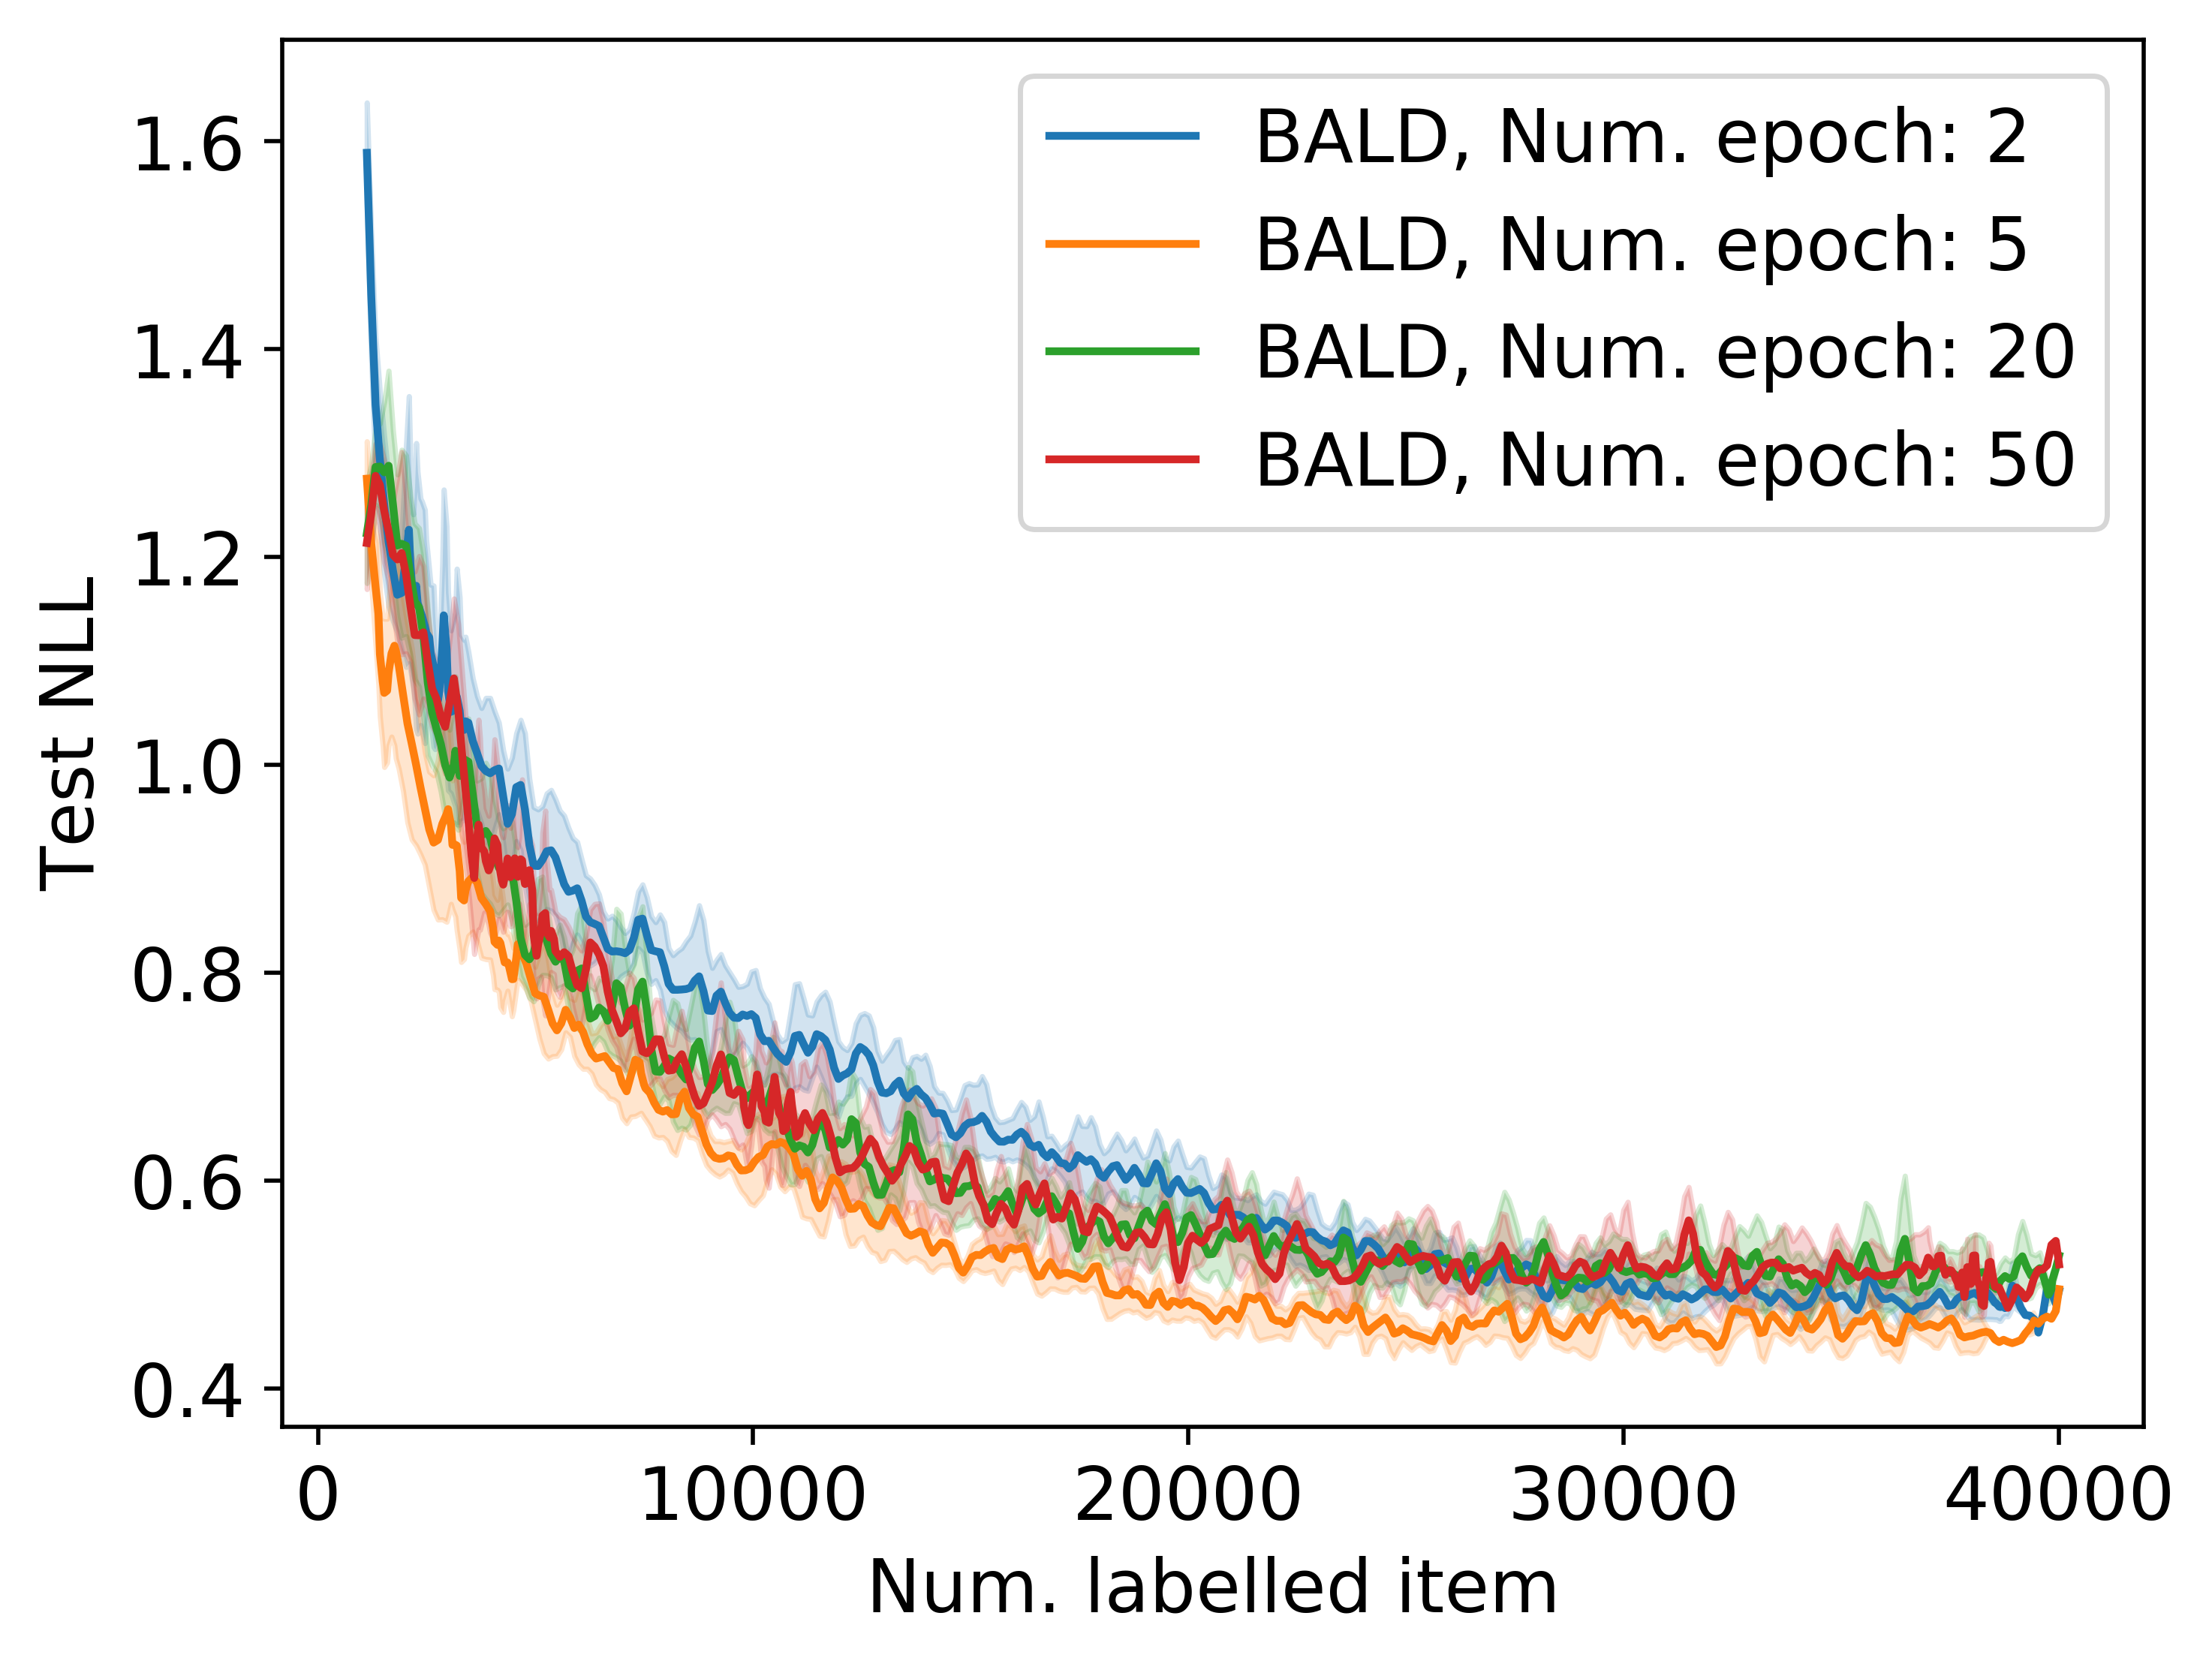
\includegraphics[width=0.35\textwidth]{fig/lrn_epoch.png}
    \caption{Effect of different training schedules. By comparing overfitted and underfitted models, we assess the impact of uncertainty quality on active learning. Performance averaged over 5 runs.}
    \label{fig:convergence}
\end{figure}


% \paragraph{Imbalanced datasets}

% How to deal with imbalanced datasets is an entire area of research \citep{krawczyk2016learning}, but little has been done to deal with it when we are not aware of the \textit{a priori} class distribution. In consequence, the active learning model may quickly overfit to the more popular classes and reduce the effectiveness of active learning procedure. From \citet{gal2017deep}, it is known that Bayesian active learning will favor underrepresented classes. But, we find the reported experiments to too simple. We  test this hypothesis in a controlled environment where we can set the amount of unrepresented classes. 

% In \tabref{fig:imbalanced}, we took the standard CIFAR100 dataset and we mimic an imbalanced dataset where few classes have a high number of examples. A class selected to be under represented sees its number of samples to be reduced by 90\%. When we increase the number of underrepresented classes, the gain of using MC-Dropout versus random sampling become more obvious. This is due to regions on the learned manifold associated with underrepresented classes to be highly uncertain. In consequence, these regions will be selected for labelling very early in the process.

% \begin{table}
%     \centering
%     \begin{tabular}{llll}
    
%     \toprule
%     Dataset size &         5000 &        10000 &        20000 \\
    
%     \hline
%   $\Delta =10$ \\
%     BALD &  4.39 \std{0.4} &  3.99 \std{0.01} &  3.57 \std{0.05} \\
%     Entropy &  4.71 \std{0.02} &  4.54 \std{0.07} &  3.94 \std{0.01} \\
%     Random &  4.52 \std{0.09} &  4.10 \std{0.03} &  3.71 \std{0.05} \\
%     \hline
%   $\Delta =25$ \\
%     BALD &  4.40 \std{0.03}	&4.04\std{0.03} &	3.61\std{0.08} \\
%     Entropy &  4.76 \std{0.02} &  4.68 \std{0.08} &   4.00 \std{0.01} \\
%     Random &  4.58 \std{0.08} &  4.18 \std{0.04} &  3.75 \std{0.01} \\
%     \hline 
%   $\Delta =50$ \\
%     BALD &  4.49 \std{0.08} &   4.07 \std{0.02} &   3.66 \std{0.04} \\
%     Entropy &  4.83 \std{0.04} &  4.60 \std{0.14} &  4.07 \std{0.28} \\
%     Random &  4.62 \std{0.03} &   4.21 \std{0.02} &   3.76 \std{0.04}
%     \end{tabular}
%     \caption{Effect of using active learning on imbalanced versions of CIFAR100. $\Delta$ is the number of class that contains 25\% of their data. From \citep{gal2017deep}, we know that BALD is robust to imbalanced datasets, but the study was not extensive. While BALD is robust to imbalanced datasets, the effect is catastrophic when using Entropy.  Performance averaged over 5 runs.}
%     \label{fig:imbalanced}
% \end{table}


% In this section, we investigated how common issues in deep learning are affecting active learning. While BALD is robust to data imbalance, it is highly affected by the annotation error or being under fitted.
In this section, we investigated the effect of two common deep learning pathologies in active learning. In summary, prior knowledge on the quality of the annotations and on how long to train the model, could help using active learning. 

\subsection{Efficient techniques for active learning}\label{techniques}

An important problem with current active learning pipelines is the delay between active learning steps. %In particular, at the beginning of the process, computing the uncertainty on the unlabelled pool of observations has a prohibitive cost. When the labelled dataset becomes large, then the cost of training the model becomes prohibitive. 
To make active learning efficient, we propose several techniques that maintain performance while speeding up the training or inference phases.

\paragraph{Query size}
An important hyper-parameter in batch active learning is to decide how many samples should be labelled at each active learning step \citep{gal2017deep, tsymbalov2019deeper}. %This parameter turns out to be vital to be set properly as \citet{tsymbalov2019deeper} as shown. 
In a real-world scenario, we can't ask the annotation team to wait between steps especially in a crowd-sourcing environment. %Of course, we do not want to label the whole pool of dataset in the next coming active learning step, and on the other extreme, we neither want to add only one sample label to the labelled subset of data. The first scenario would require labelling the whole dataset which is against the purpose of the whole framework and the latter will result in an exhaustively slow process which we obviously could not afford in a production setup. 
Therefore, there needs to be a configuration where we could benefit from a good uncertainty estimation quality and a reasonable runtime. We present our findings in \tabref{fig:query_size} where we tested this approach on CIFAR10. 
From our results, the query size does decreases performances, especially at 10,000 labels where the gap between BALD and Entropy is thinner as the query size grows.

\begin{table}
{\small
\begin{tabular}{llll}
\toprule
    Dataset size &          5000 &         10000 &         20000 \\
\midrule
\textbf{Random} &  0.71 \std{0.03} &  0.54 \std{0.01} &  0.42 \std{0.05} \\
\hline
   $\Q$=50 &                  &                  &                  \\
   \hline
            BALD &  0.59 \std{0.01} &  0.46 \std{0.05} &  0.34 \std{0.02} \\
         Entropy &  0.69 \std{0.06} &  0.55 \std{0.11} &  0.34 \std{0.00} \\
          \hline
  $\Q$=250 &                  &                  &                  \\
  \hline
            BALD &  0.61 \std{0.03} &  0.43 \std{0.01} &  0.35 \std{0.03} \\
         Entropy &  0.67 \std{0.05} &  0.49 \std{0.04} &  0.35 \std{0.00} \\
          \hline
  $\Q$=500 &                  &                  &                  \\
  \hline
            BALD &  0.61 \std{0.07} &  0.42 \std{0.02} &  0.36 \std{0.01} \\
         Entropy &  0.61 \std{0.07} &  0.47 \std{0.00} &  0.37 \std{0.00} \\
          \hline
 $\Q$=2000 &                  &                  &                  \\
 \hline
            BALD &  0.77 \std{0.05} &  0.53 \std{0.03} &  0.37 \std{0.03} \\
         Entropy &  0.87 \std{0.01} &  0.52 \std{0.07} &  0.35 \std{0.01} \\
\bottomrule
\end{tabular}}



    \centering
    \caption{Effect of increasing the query size $\Q$ on CIFAR10. Performance averaged over 5 runs. BALD is weaker when used with a large query size, making Entropy competitive.}
    \label{fig:query_size}
\end{table}

\paragraph{Limit pool size}

The most time-consuming part of active learning is the uncertainty estimation step. In particular, this step is expensive when using techniques that require Monte-Carlo sampling such as MC-Dropout or Bayesian neural networks. 
Of course, this problem is embarrassingly parallel, but for low-budget deployment, one has not access to the resources required to parallelize this task cheaply.
A simple idea to solve this is to randomly select unlabelled samples from the pool instead of using the entire pool. We test this idea by varying the number of samples selected for uncertainty estimation. 
%In \figref{fig:pool_size}, we show that there is no difference between choosing between the entire pool or less than 25\%. This shows that one can heavily speed up the inference phase by limiting the size of the pool
From our experiments (figure in Annex), we show that the performance is not affected when using less than 25\% of the pool. By doing this, we can speed up this phase by a factor of 3.

In this section, we proposed two approaches to make active learning usable in production. First, we can increase the query size higher than previously used in the literature. Second, we can select the next batch using a small subset of the pool.

% \begin{figure}
%     \centering
%     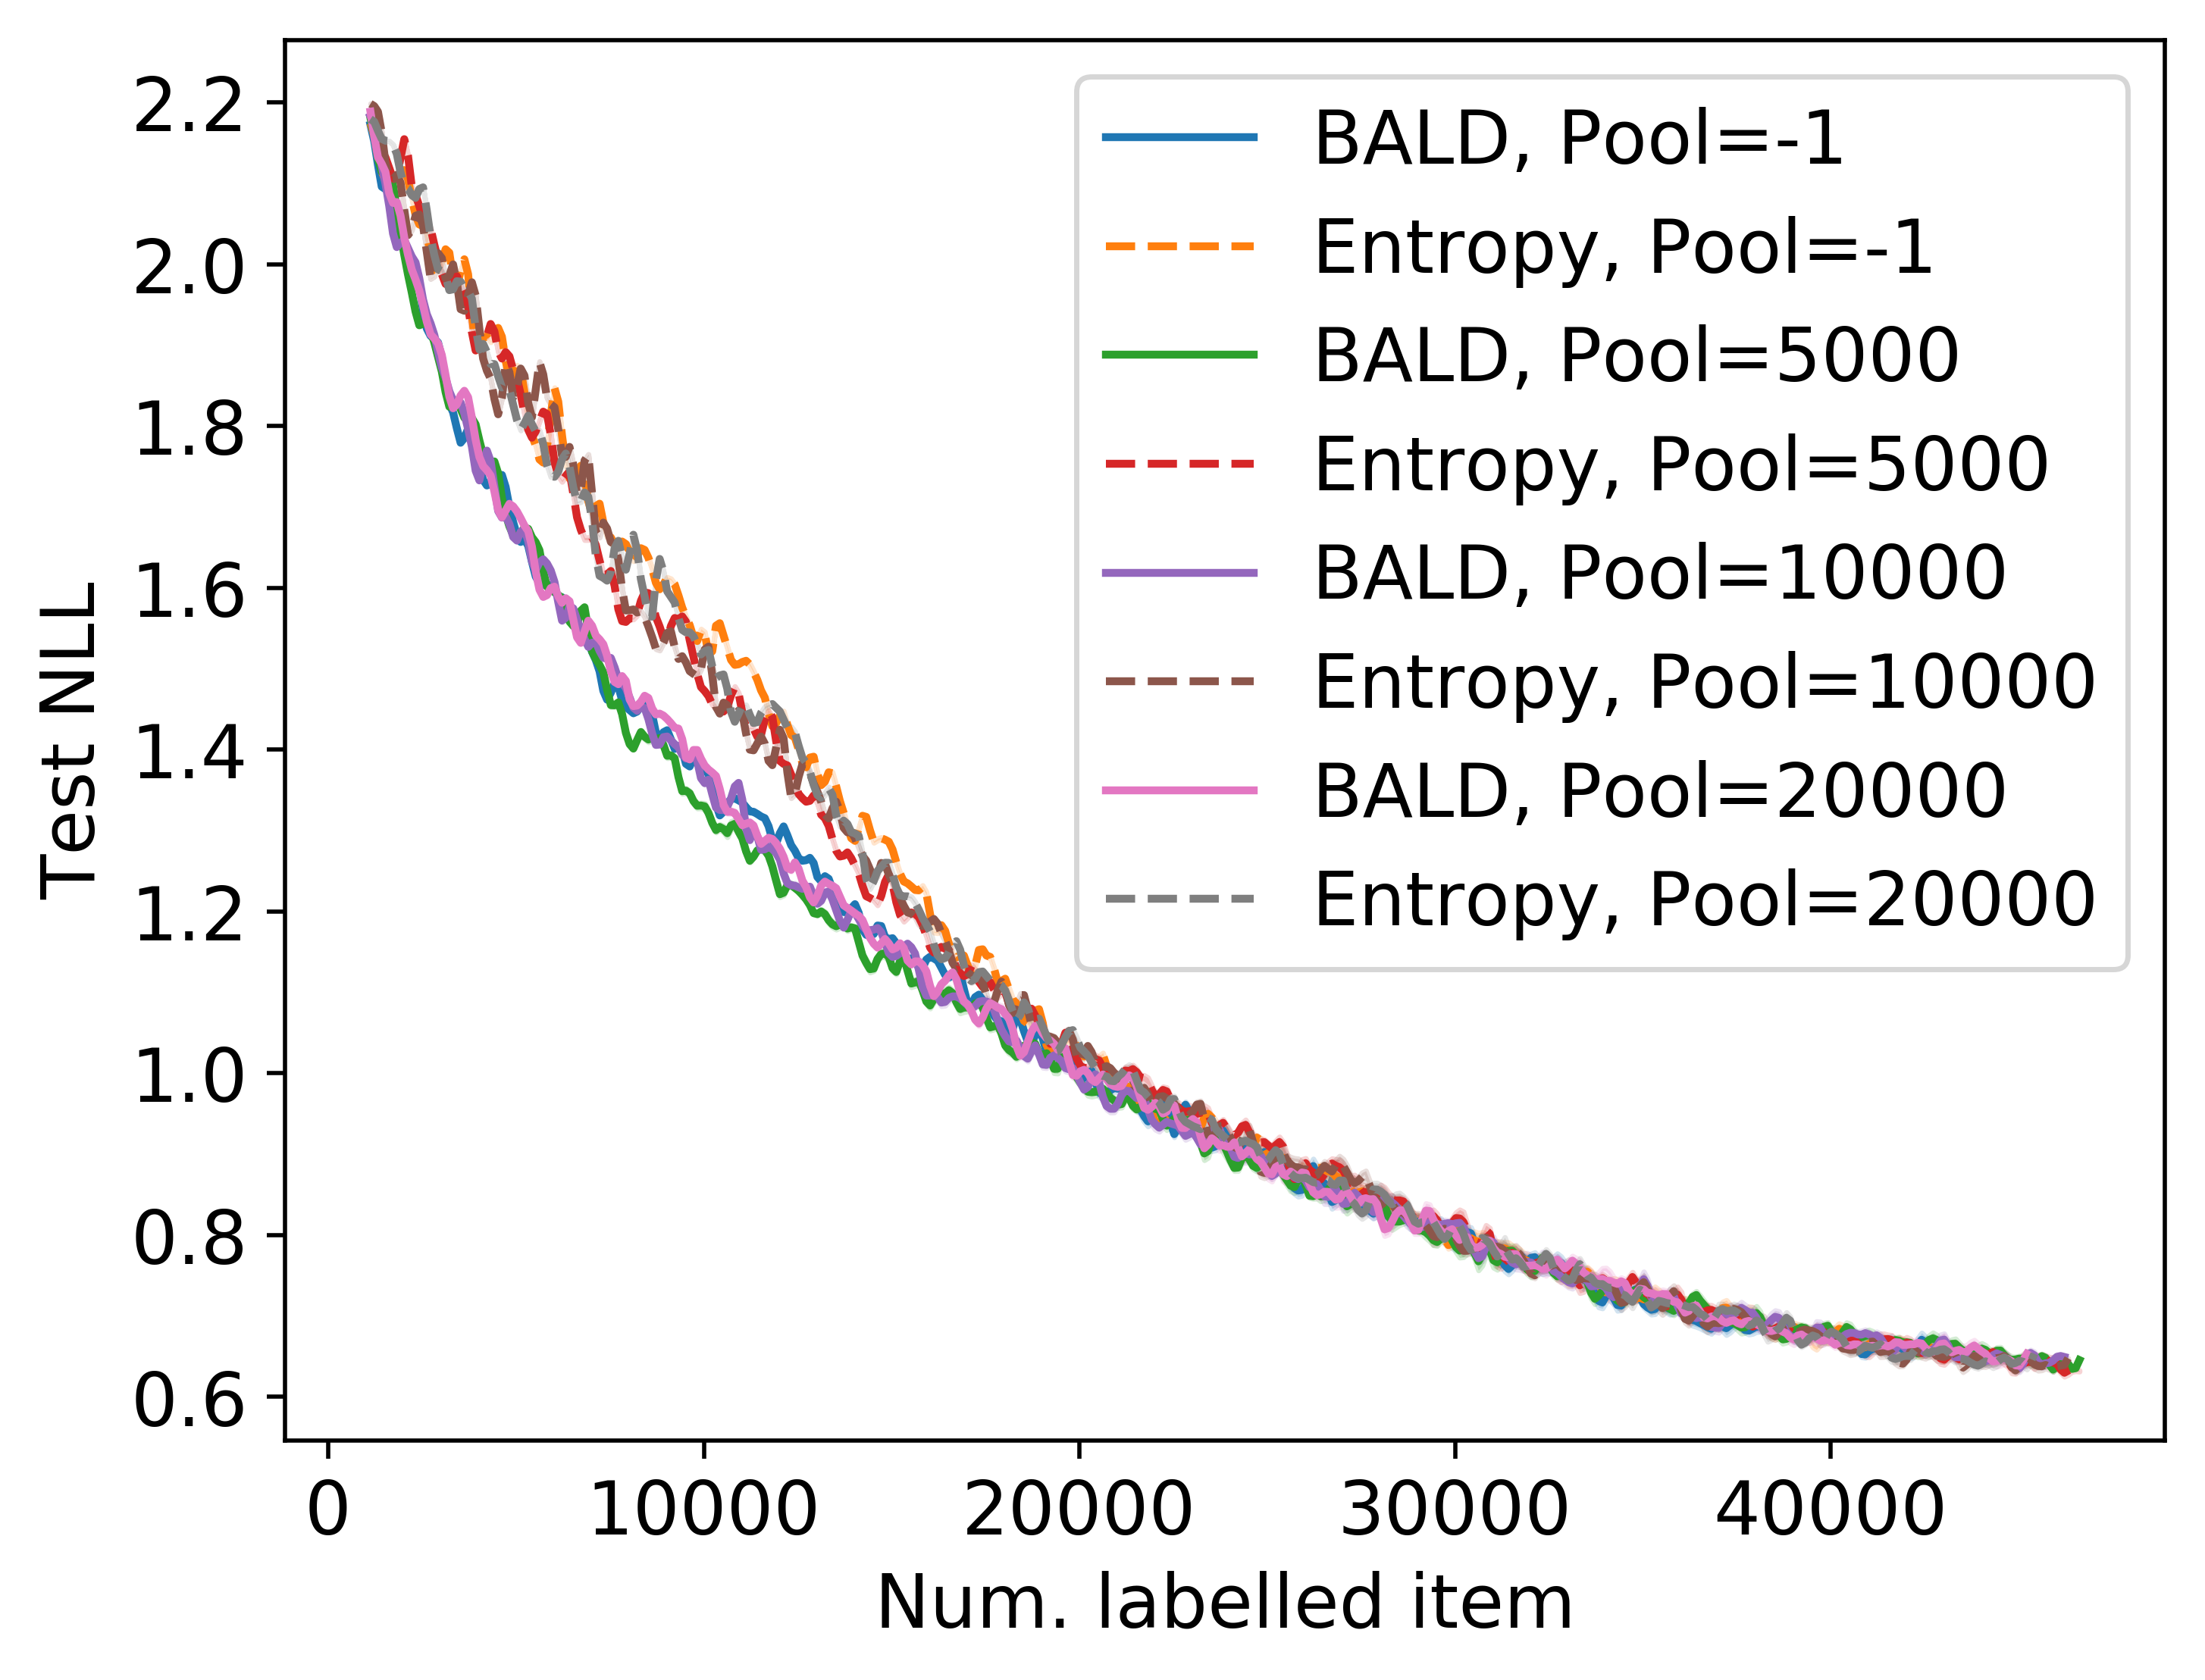
\includegraphics[width=0.4\textwidth]{fig/pol_size.png}
%     \caption{Effect of reducing the size of the pool on CIFAR10. \textbf{-1} indicates no reduction. For all heuristics, the performance is not affected by the size of the pool showing that AL can be efficient when tuned properly.  Performance averaged over 5 runs.}
%     \label{fig:pool_size}
% \end{figure}

\section{Case study: Mio-TCD}

Few datasets have been proposed to mimic a "real-world" situation where the dataset suffers from labelling noise, duplicates, or imbalanced datasets. Mio-TCD \citep{luo2018mio} has been recently proposed to showcase these issues. The dataset contains 500,000 samples split into 11 classes with heavy class imbalance. For example, the training set contains 50\% \textit{Cars} and 20\% \textit{Background}. 

\paragraph{Benefits of active learning.}
As shown in \citet{gal2017deep} (and further in Annex), active learning helps when used on imbalanced data. We can verify this, by comparing the performance of underrepresented classes in Mio-TCD. From the current leader board, we can select two difficult classes: \textit{Single-Unit Truck, and Bicycle}. We use the same setup as before, but limit the size of the pool to 20,000 samples. %Comparing the results in \figref{fig:standard}, BALD is clearly superior which further validates the need for better benchmarks in active learning.



% \subsubsection{Adding random noise to the selection}

% We first analyze the impact of the proposition of \citet{dasgupta2011two} to add noise when selecting the next samples to label.
% In this highly imbalanced dataset, we make the hypothesis that it would be highly valuable as it is likely that some classes are not represented in the initial random sampling. Furthermore, at each active learning step, the pool of unlabelled data would be ranked based on model uncertainty before selecting the samples to be labeled. In this setting, two classes can be highly confused and ,depending on the selection process, still be highly confident predictions.

% Furthermore, as \citet{lowell2019practical} has demonstrated, datasets labelled using active learning are good to train deep learning models, but not so much when training models from different paradigms. % ICML CUT new paper By adding noise to the selection, we hope to remove some part of the selection bias added to the dataset.
\begin{figure}
    \centering
    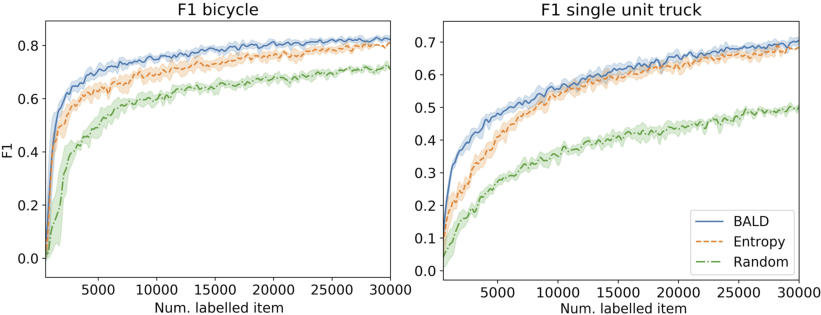
\includegraphics[width=0.5\textwidth]{fig/F1_Miotcd_top.pdf}
    \caption{Performance of different active learning procedures on Mio-TCD. While any active learning method is strong against random, BALD is especially strong at the beginning of the labelling process.  Performance averaged over 5 runs.}
    \label{fig:mioclasses}
\end{figure}
% However, what model chooses to be most valuable in the next round of training is not necessarily diverse enough and could be concentrated on part of the data which is simply harder to decode for the model. Continuing in adding samples solely based on model uncertainty feedback, could eventually teach the model to learn the most uncertain part of the data while the least uncertain part do not get any representation in the bigger scale and hence model would fail in learning the whole data distribution\cite{dasgupta2011two}. 

In \figref{fig:mioclasses}, we present the F1 scores for the two most difficult classes. One can clearly see the impact of using active learning in this setting. With active learning, underrepresented classes are quickly selected and get decent performance. In addition, the performance for the most populous class \textit{Cars} stays similar across acquisition functions (figure in Annex). 

%ICML CUT no gain actually Given the percentage of noise, we randomly swap samples from the ranked set of pool. For example, choosing to label 100 samples at each active learning step with 10\% noise means that 90 data point will be labelled based on model uncertainty decision and 10 data points will be labelled randomly. Using this method is especially useful for \textit{entropy} which is weaker than BALD. On the contrary, BALD is not affected by this method, but it does not get hurt it either.

This experiment shows that using active learning on non-academic datasets is highly beneficial and the need for the active learning community to use new benchmarks to compare methods.





\section{Conclusion}

In this paper, we have investigated the impact of uncleaned data on deep active learning models used for active learning. We also propose several techniques to make active learning usable in a real-world environment. Subsequently, we test our findings on a real-world dataset Mio-TCD, showing that active learning can be used in this setting.  As a result of this study, we introduce our newly released Bayesian active learning library which can be useful to both researchers and developers (see Annex).


In summary, we show that active learning can be used in a production setting on real data with success. We hope this work can fasten the application of active learning on real-world projects and improve the quality of annotation by getting more information per sample. Interesting areas of research include the study of the interaction between the human and the machine during a labelling task.

\clearpage
\bibliography{example_paper}
\bibliographystyle{icml2020}
% For submission, needs to be 2 documents and then concat together.
\appendix
%%%%%%%% ICML 2020 EXAMPLE LATEX SUBMISSION FILE %%%%%%%%%%%%%%%%%

\documentclass{article}
\usepackage{times}
\usepackage{epsfig}
\usepackage{graphicx}
\usepackage{amsmath}
\usepackage{amssymb}
\usepackage{times}
\usepackage{epsfig}
\usepackage{graphicx}
\usepackage{amsmath}
\usepackage{amssymb}
% Include other packages here, before hyperref.
\usepackage{xcolor}
\usepackage[ruled,vlined,onelanguage]{algorithm2e}
\usepackage{setspace}
\usepackage{collcell}
\usepackage{xr}
\usepackage{natbib}
\usepackage{multirow}
\usepackage{subcaption}
\usepackage{mathtools}
\usepackage{colortbl,dcolumn}
\usepackage{algorithm2e}

% Include other packages here, before hyperref.

% If you comment hyperref and then uncomment it, you should delete
% egpaper.aux before re-running latex.  (Or just hit 'q' on the first latex
% run, let it finish, and you should be clear).
\usepackage[pagebackref=true,breaklinks=true,letterpaper=true,colorlinks,bookmarks=false]{hyperref}

% \cvprfinalcopy % *** Uncomment this line for the final submission

\def\cvprPaperID{****} % *** Enter the CVPR Paper ID here
\def\httilde{\mbox{\tt\raisebox{-.5ex}{\symbol{126}}}}

\newcommand{\todo}[1]{{\color{blue}TODO #1}}
\newcommand{\toref}[1]{{\color{red}REF #1 }}
\newcommand{\registered}{\textsuperscript{\tiny\textregistered}}
%\newcommand{\etal}{\textit{et al.}}
\renewcommand{\eqref}[1]{\hyperref[#1]{Eq.\ \ref*{#1}}}
\newcommand{\figref}[1]{\hyperref[#1]{Fig.\ \ref*{#1}}}
\newcommand{\tabref}[1]{\hyperref[#1]{Table\ \ref*{#1}}}
\newcommand{\secref}[1]{\hyperref[#1]{Section\ \ref*{#1}}}
\newcommand{\algoref}[1]{\hyperref[#1]{Algorithm\ \ref*{#1}}}
\newcolumntype{C}[1]{>{\centering}m{#1}}
\newcommand{\N}{{\cal N}}
\newcommand{\std}[1]{ \normalfont \color{darkgray}\footnotesize{$\pm$#1} }

% SYMBOL
\newcommand{\E}{{\mathbb E}}

\hypersetup{
    colorlinks=true,
    linkcolor=blue,
    filecolor=magenta,      
    urlcolor=blue,
}

\urlstyle{same}

% Recommended, but optional, packages for figures and better typesetting:
\usepackage{microtype}
\usepackage{booktabs} % for professional tables

% hyperref makes hyperlinks in the resulting PDF.
% If your build breaks (sometimes temporarily if a hyperlink spans a page)
% please comment out the following usepackage line and replace
% \usepackage{icml2020} with \usepackage[nohyperref]{icml2020} above.
\usepackage{hyperref}

% Attempt to make hyperref and algorithmic work together better:
\newcommand{\theHalgorithm}{\arabic{algorithm}}

% Use the following line for the initial blind version submitted for review:
%\usepackage{icml2020}

% If accepted, instead use the following line for the camera-ready submission:
\usepackage[accepted]{icml2020}

% The \icmltitle you define below is probably too long as a header.
% Therefore, a short form for the running title is supplied here:
\icmltitlerunning{Bayesian active learning for production. Supplementary Material}

\begin{document}

\twocolumn[
\icmltitle{Supplementary Material}]

\section{Implementation details}
Our methodology is as follows. We train a VGG-16 \citep{zhang2015accelerating} pretrained on ImageNet~\citep{imagenet_cvpr09}. Our initial training set contains 500 samples. We estimate the uncertainty using 20 MC samples and label the 100 most uncertain elements. Following \citet{gal2017deep}, we reset the weights to their initial value between steps. 

\section{Imbalanced datasets}
 
How to deal with imbalanced datasets is an entire area of research \citep{krawczyk2016learning}, but little has been done to deal with it when we are not aware of the \textit{a priori} class distribution. In consequence, the active learning model may quickly overfit to the more popular classes and reduce the effectiveness of active learning procedure. From \citet{gal2017deep}, it is known that Bayesian active learning will favor underrepresented classes. But, we find the reported experiments to be too simple. We  test this hypothesis in a controlled environment where we can set the number of unrepresented classes. 

In \tabref{fig:imbalanced}, we took the standard CIFAR100 dataset and we mimic an imbalanced dataset where few classes have a high number of examples. A class selected to be underrepresented sees its number of samples to be reduced by 75\%. When we increase the number of underrepresented classes, the gain of using MC-Dropout versus random sampling becomes more obvious. This is due to regions on the learned manifold associated with underrepresented classes to be highly uncertain. In consequence, these regions will be selected for labelling very early in the process.

% In this section, we investigated how common issues in deep learning are affecting active learning. While BALD is robust to data imbalance, it is highly affected by the annotation error or being under fitted.


\begin{table}
    \centering
    \begin{tabular}{llll}
    
    \toprule
    Dataset size &         5000 &        10000 &        20000 \\
    
    \hline
   $\Delta =10$ \\
    BALD &  4.39 \std{0.4} &  3.99 \std{0.01} &  3.57 \std{0.05} \\
    Entropy &  4.71 \std{0.02} &  4.54 \std{0.07} &  3.94 \std{0.01} \\
    Random &  4.52 \std{0.09} &  4.10 \std{0.03} &  3.71 \std{0.05} \\
    \hline
   $\Delta =25$ \\
    BALD &  4.40 \std{0.03}	&4.04\std{0.03} &	3.61\std{0.08} \\
    Entropy &  4.76 \std{0.02} &  4.68 \std{0.08} &   4.00 \std{0.01} \\
    Random &  4.58 \std{0.08} &  4.18 \std{0.04} &  3.75 \std{0.01} \\
    \hline 
   $\Delta =50$ \\
    BALD &  4.49 \std{0.08} &   4.07 \std{0.02} &   3.66 \std{0.04} \\
    Entropy &  4.83 \std{0.04} &  4.60 \std{0.14} &  4.07 \std{0.28} \\
    Random &  4.62 \std{0.03} &   4.21 \std{0.02} &   3.76 \std{0.04} \\
    \end{tabular}
    \caption{Effect of using active learning on imbalanced versions of CIFAR100. $\Delta$ is the number of class that contains 25\% of their data. From \citep{gal2017deep}, we know that BALD is robust to imbalanced datasets, but the study was not extensive. While BALD is robust to imbalanced datasets, the effect is catastrophic when using Entropy.  Performance averaged over 5 runs.}
    \label{fig:imbalanced}
\end{table}

\section{Effect of convergence}

In \figref{fig:active_gain}, we computed the difference in performance between BALD and random. We call this measure the \textit{Active gain} $= NLL_{Random} - NLL_{BALD}$. When using an underfitted model, the gain goes negative i.e. you would be better to use random selection.

\begin{figure}
    \centering
    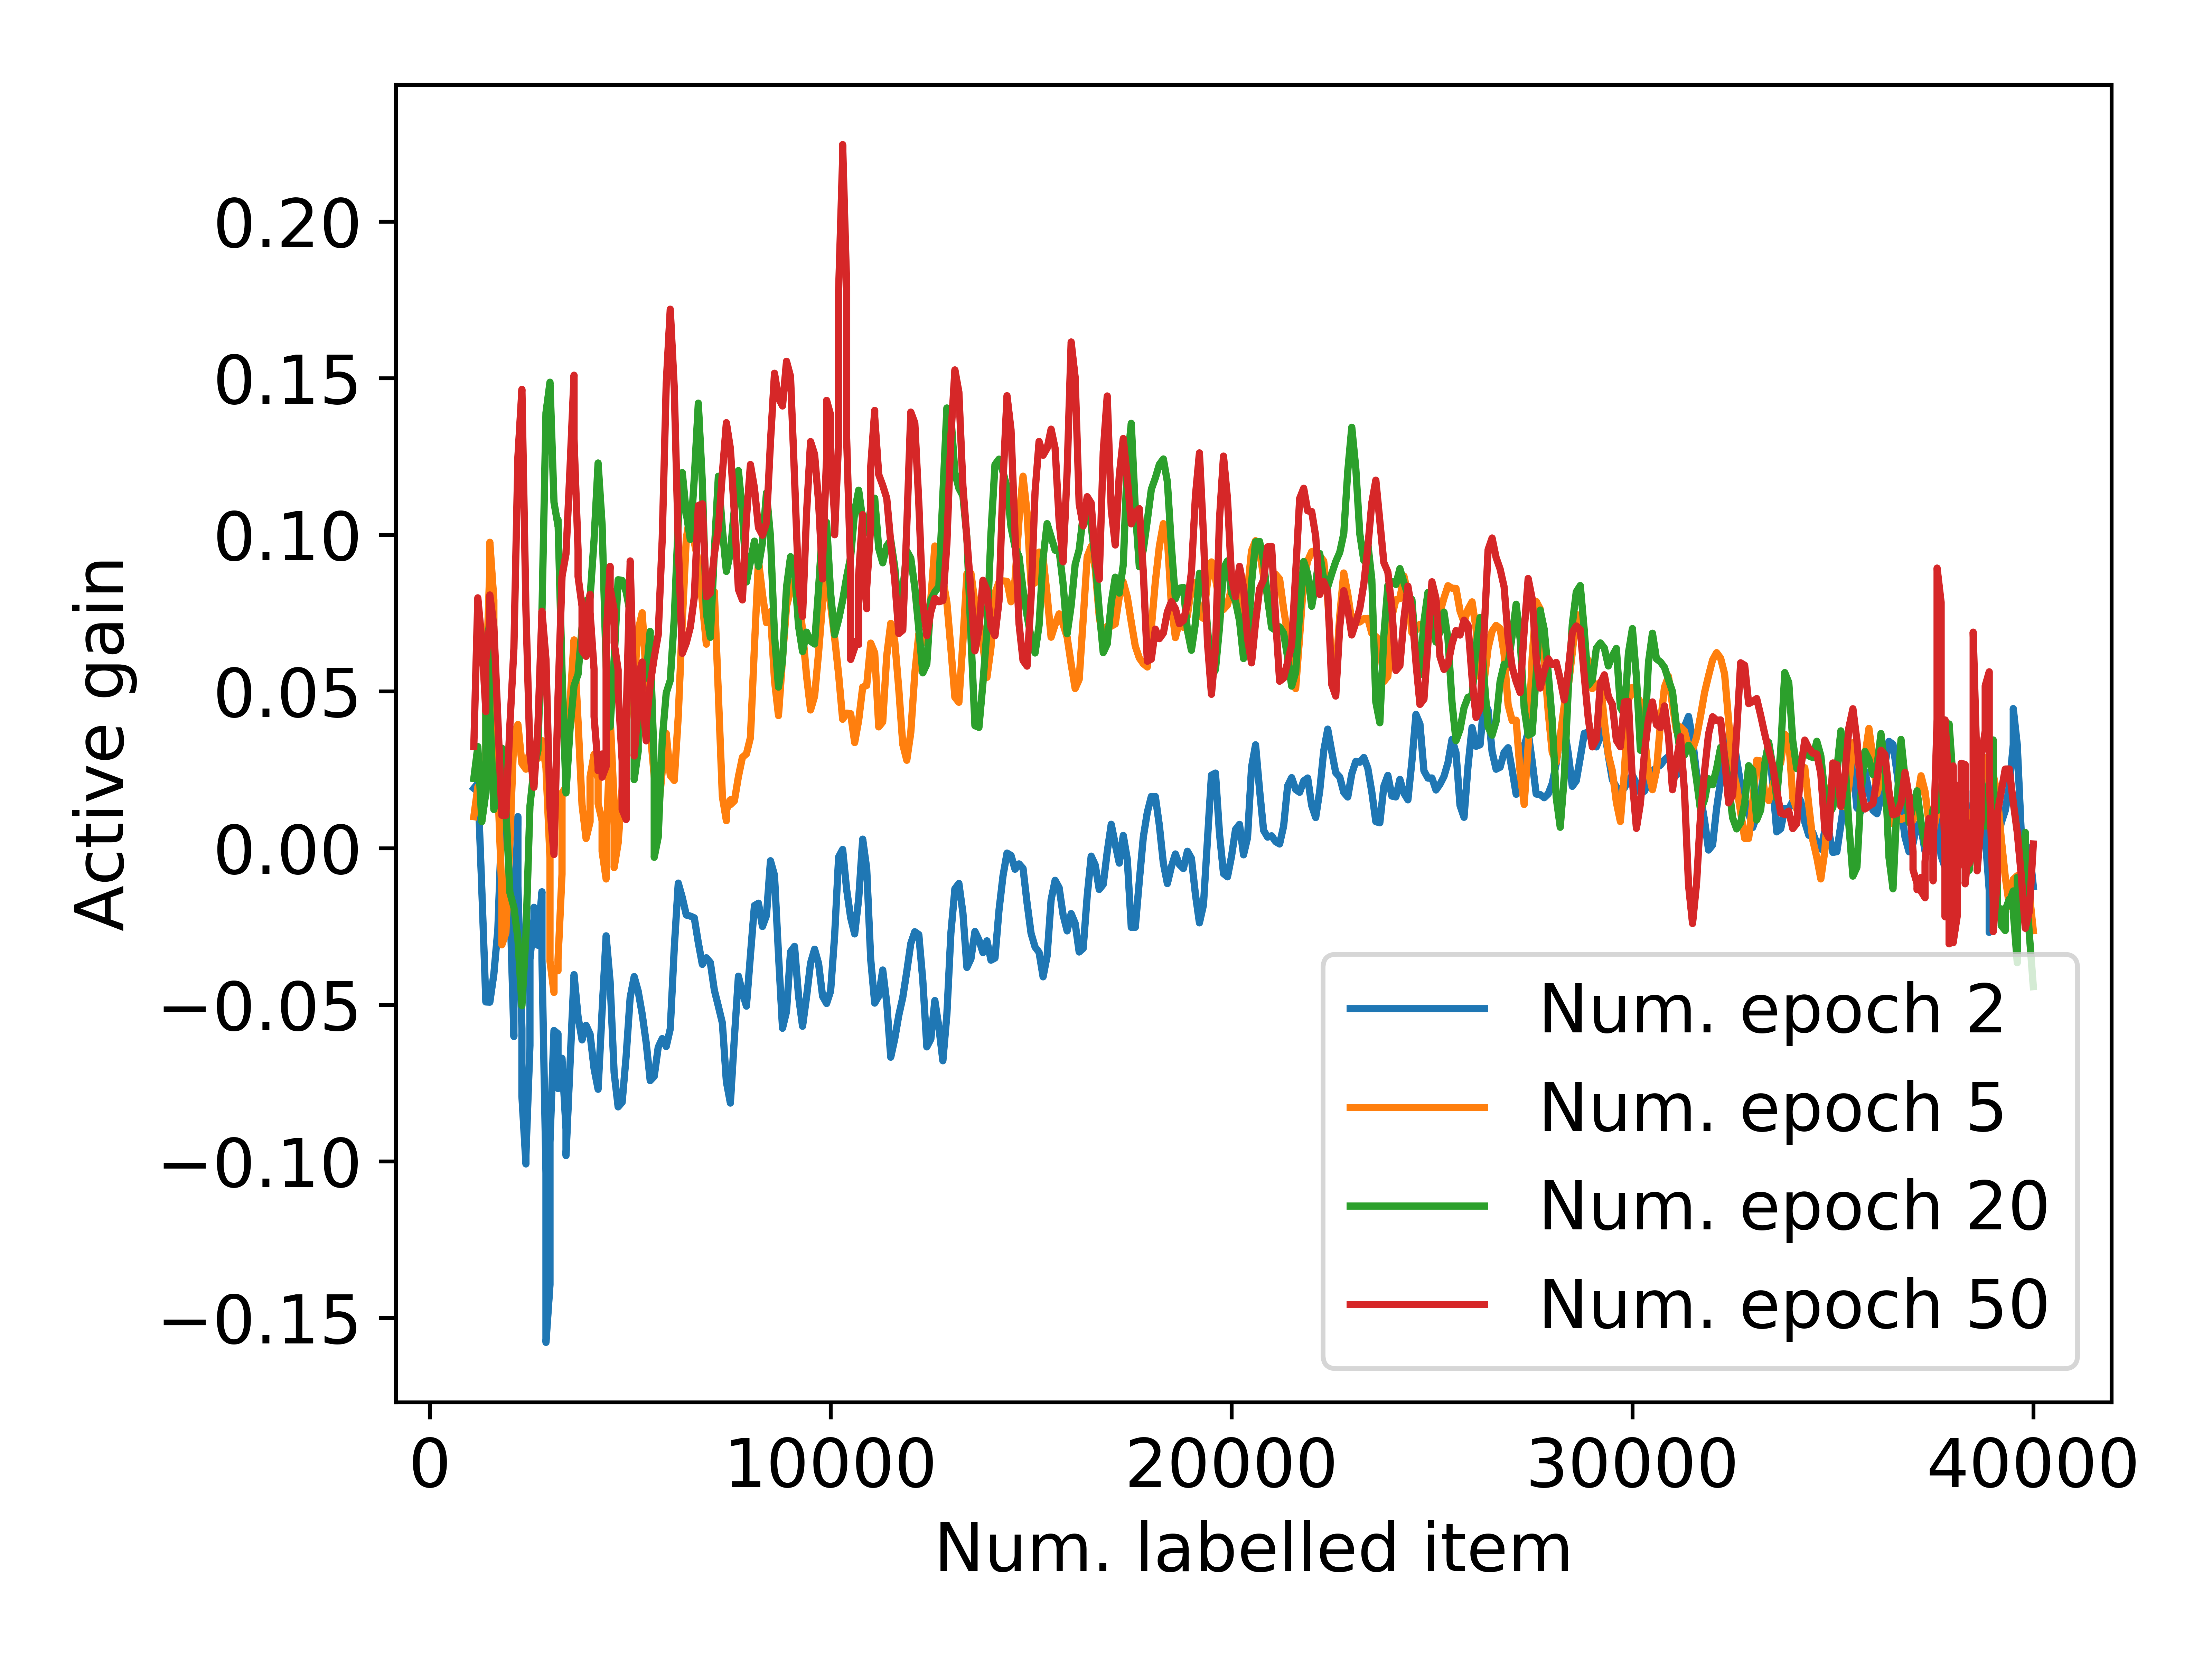
\includegraphics[width=0.5\textwidth]{fig/active_gain.png}
    \caption{Gain of using active learning when varying the number of training epochs. An underfitted model will cause harm to the model training and in this case, just using random would've been better.}
    \label{fig:active_gain}
\end{figure}

\section{Effect of reducing the pool size}
As part of the experiments, we test whether limiting the pool size would affect the performance of active learning. Our experiments in  \figref{fig:pool_size} show that whether to calculate the uncertainty for the whole pool data or a randomly selected subset, the performance of active learning is not affected. This leads to an the interesting outcome of limiting the uncertainty calculations (which is the most expensive part of an active learning loop) in production setup for faster active learning loops.

\begin{figure}
    \centering
    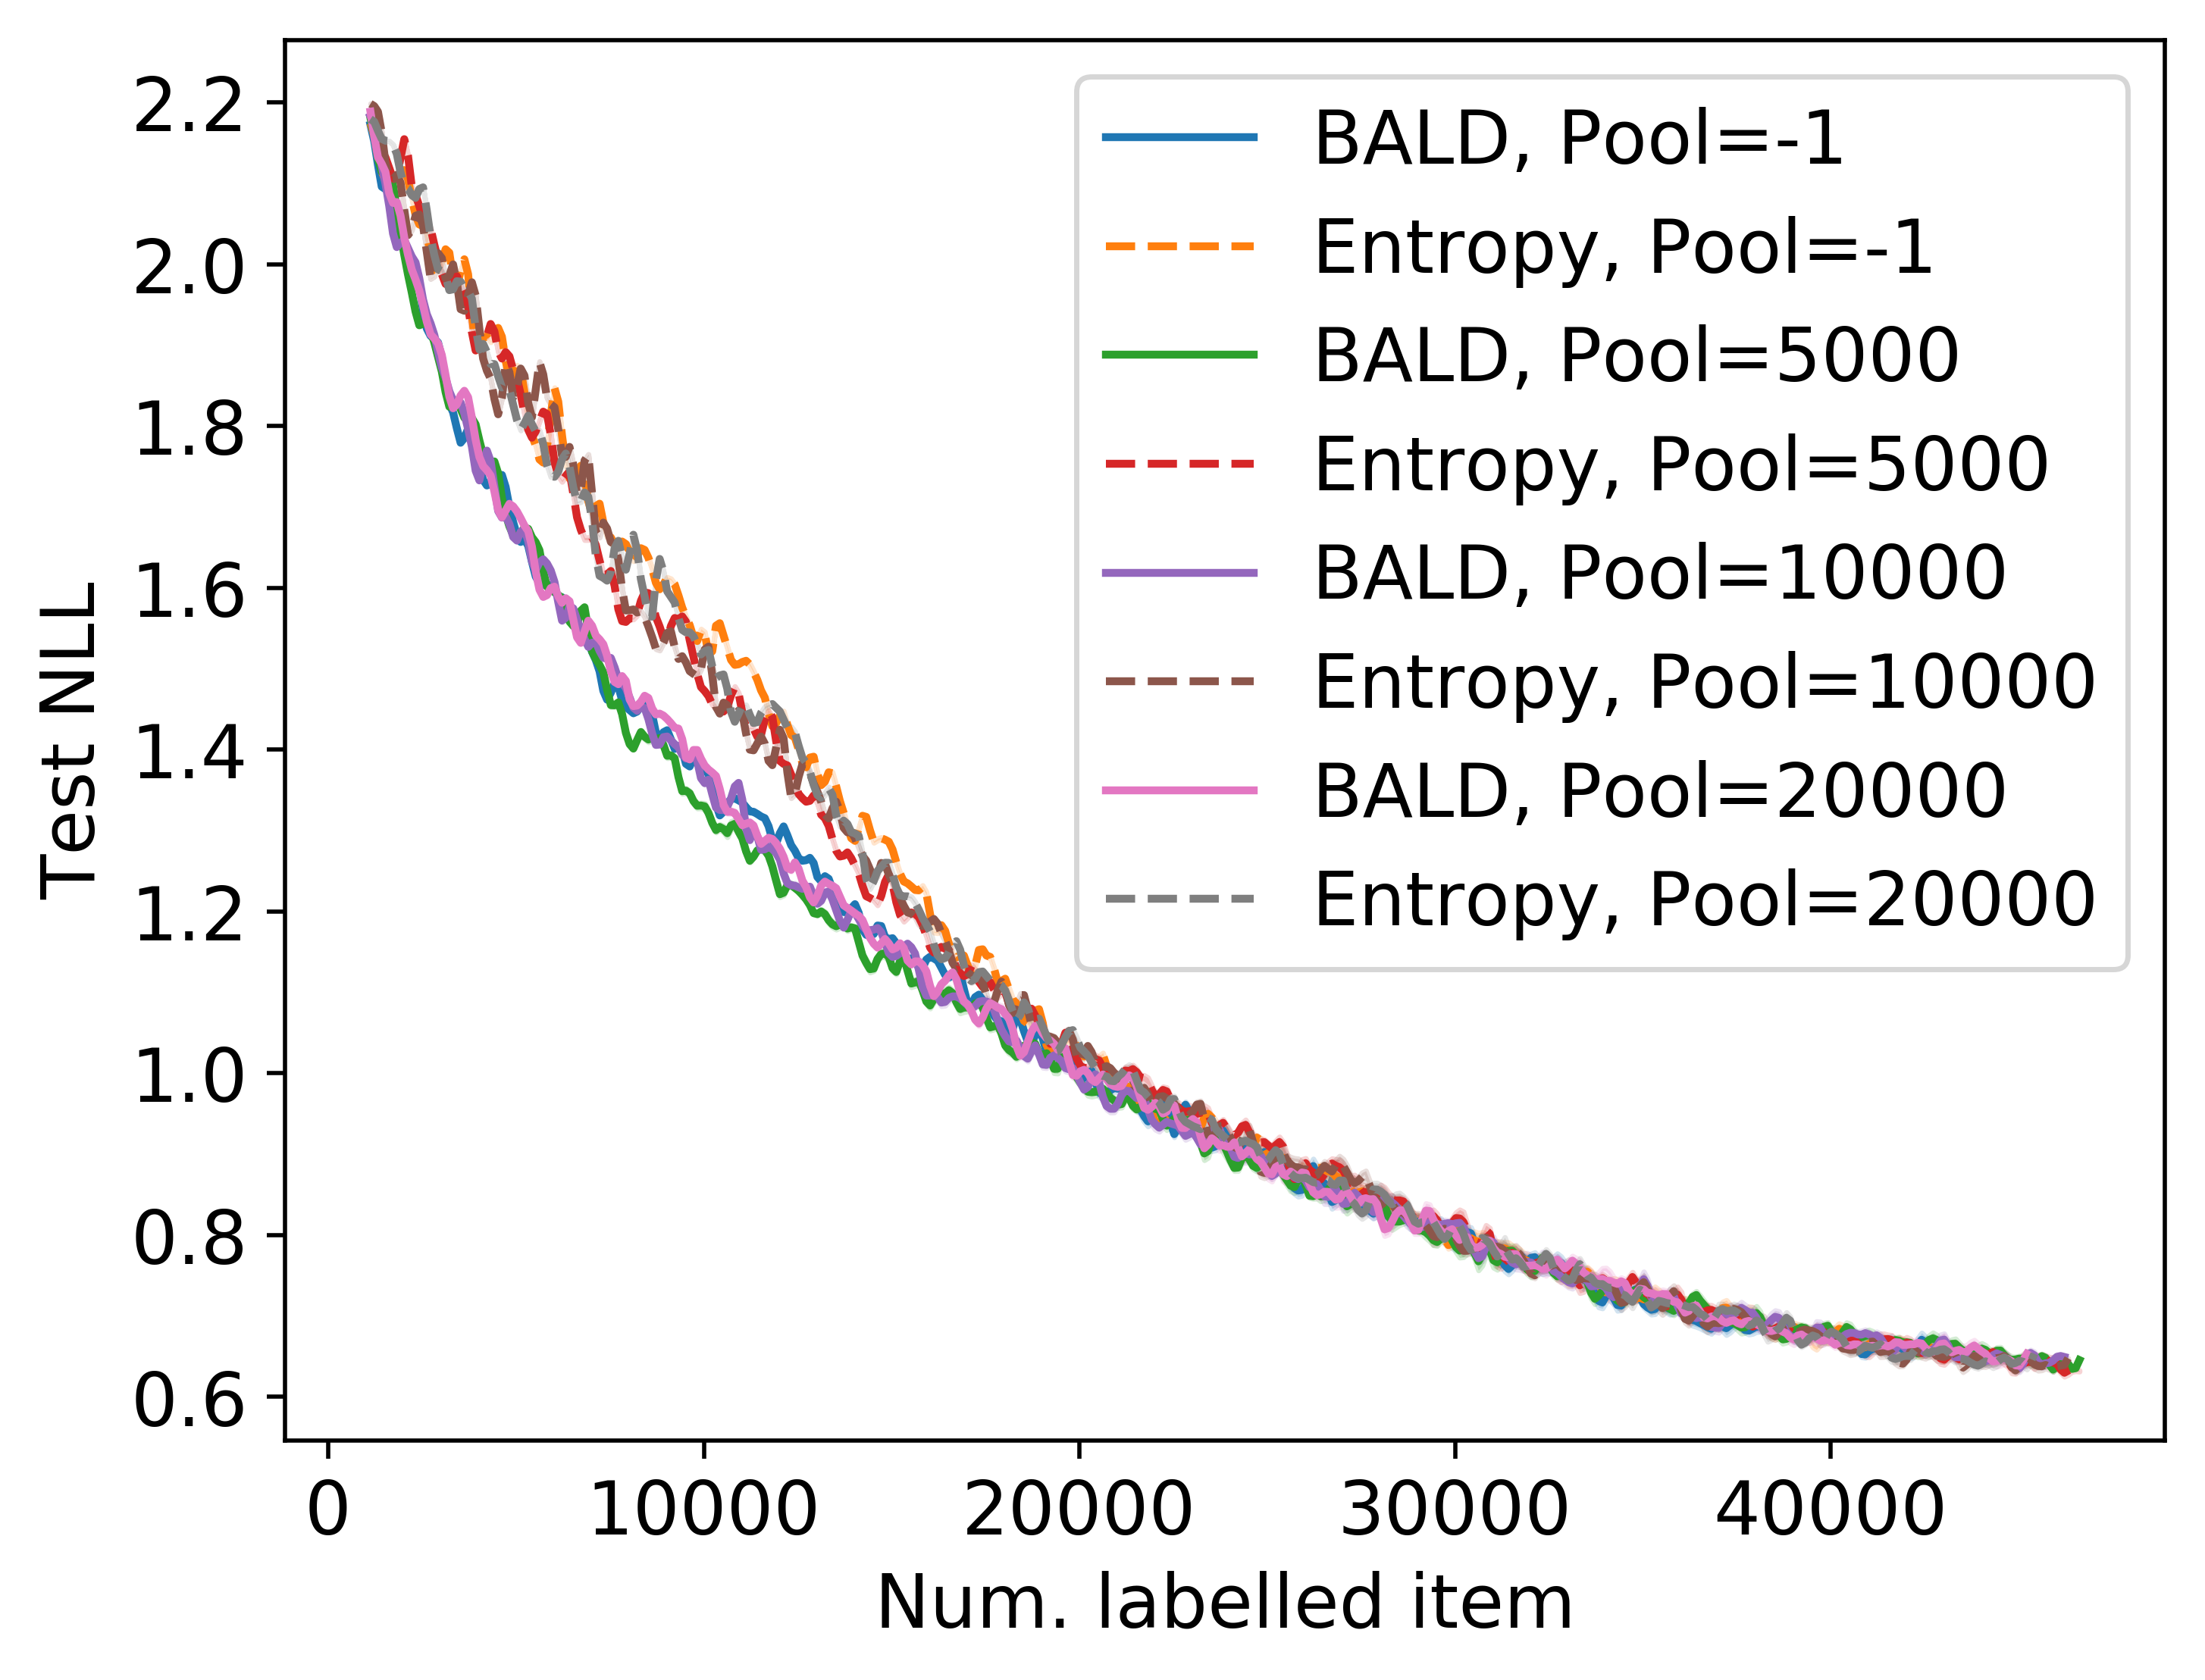
\includegraphics[width=0.4\textwidth]{fig/pol_size.png}
    \caption{Effect of reducing the size of the pool on CIFAR100. \textbf{-1} indicates no reduction. For all heuristics, the performance is not affected by the size of the pool showing that AL can be efficient when tuned properly.  Performance averaged over 5 runs.}
    \label{fig:pool_size}
\end{figure}

\begin{figure}
    \centering
    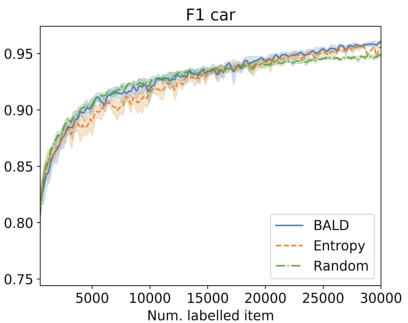
\includegraphics{fig/F1_Mio_tcd_annex.pdf}
    \caption{\textbf{F1 for the class \textit{car}}. BALD is great for underrepresented classes while not affecting more popular classes. Entropy decreases the performance on this class.}
    \label{fig:miotcd}
\end{figure}


\section{Bayesian active learning Library (BaaL)}

All the experiments in this paper have done using our publicly available Bayesian active learning library.  The goal of this library is to provide an easy to use but complete setup to test active learning on any project with few lines of code. We included features that current active learning libraries do not support. In particular, Bayesian methods such as MC-Dropout or Coresets are not widely available and there is no standard implementation of the active learning loop. Furthermore, research codebases are often hard to read and hard to maintain. Our proposed unified API could satisfy both research and industrial users.

 Our recently published open-source package named BaaL, aims at accelerating the transition from research to production. The core philosophy behind our library is to provide researchers with a well-designed API so that they focus on their novel idea and not on technical details. Our library proposes a task-agnostic system where one can mix-and-match any set of acquisition functions and uncertainty estimation methods.
The library consists of three main components:
\begin{enumerate}
    \item Dataset management to keep track and manage the labelled data $D_L$ and the unlabelled data $D_U$.
    \item Bayesian Methods i.e. MC-Dropout, MC-DropConnect and so on.
    \item Acquisition functions i.e. BALD, BatchBALD, Entropy and more.
\end{enumerate}

We provide full support for Pytorch \cite{paszke2017automatic} deep learning modules but our acquisition functions which are the most important part of active learning is implemented in  Numpy\cite{oliphant2006guide} and hence can be used on any platform. Our Data management module keeps track of what is labelled and what is unlabelled. We also provide facilitator methods to label a data point, update the pool of unlabelled data, and to randomly label a portion of the dataset. In our Bayesian module, we provide utilities to make any Pytorch model Bayesian with a single instruction. We also provide training, testing, and active learning loops that facilitate the active training procedure. Our acquisition functions are up-to-date with state-of-the-art methods. We provide easy to follow tutorials (https://baal.readthedocs.io/en/latest/) for each section of the library so that the user understands how each component works. Finally, our library is a member of Pytorch Ecosystem, which is reserved for libraries with outstanding documentation.

Our road-map has been indicated in the repository. Our current focus will include model calibration and semi-supervised learning. As more researchers contribute their methods to our library, we aim to become the standard Bayesian active learning library.

\end{document}
\end{document}



% This document was modified from the file originally made available by
% Pat Langley and Andrea Danyluk for ICML-2K. This version was created
% by Iain Murray in 2018, and modified by Alexandre Bouchard in
% 2019 and 2020. Previous contributors include Dan Roy, Lise Getoor and Tobias
% Scheffer, which was slightly modified from the 2010 version by
% Thorsten Joachims & Johannes Fuernkranz, slightly modified from the
% 2009 version by Kiri Wagstaff and Sam Roweis's 2008 version, which is
% slightly modified from Prasad Tadepalli's 2007 version which is a
% lightly changed version of the previous year's version by Andrew
% Moore, which was in turn edited from those of Kristian Kersting and
% Codrina Lauth. Alex Smola contributed to the algorithmic style files.

%%%%%%%% ICML 2020 EXAMPLE LATEX SUBMISSION FILE %%%%%%%%%%%%%%%%%

\documentclass{article}
\usepackage{times}
\usepackage{epsfig}
\usepackage{graphicx}
\usepackage{amsmath}
\usepackage{amssymb}
\usepackage{times}
\usepackage{epsfig}
\usepackage{graphicx}
\usepackage{amsmath}
\usepackage{amssymb}
% Include other packages here, before hyperref.
\usepackage{xcolor}
\usepackage[ruled,vlined,onelanguage]{algorithm2e}
\usepackage{setspace}
\usepackage{collcell}
\usepackage{xr}
\usepackage{natbib}
\usepackage{multirow}
\usepackage{subcaption}
\usepackage{mathtools}
\usepackage{colortbl,dcolumn}
\usepackage{algorithm2e}

% Include other packages here, before hyperref.

% If you comment hyperref and then uncomment it, you should delete
% egpaper.aux before re-running latex.  (Or just hit 'q' on the first latex
% run, let it finish, and you should be clear).
\usepackage[pagebackref=true,breaklinks=true,letterpaper=true,colorlinks,bookmarks=false]{hyperref}

% \cvprfinalcopy % *** Uncomment this line for the final submission

\def\cvprPaperID{****} % *** Enter the CVPR Paper ID here
\def\httilde{\mbox{\tt\raisebox{-.5ex}{\symbol{126}}}}

\newcommand{\todo}[1]{{\color{blue}TODO #1}}
\newcommand{\toref}[1]{{\color{red}REF #1 }}
\newcommand{\registered}{\textsuperscript{\tiny\textregistered}}
%\newcommand{\etal}{\textit{et al.}}
\renewcommand{\eqref}[1]{\hyperref[#1]{Eq.\ \ref*{#1}}}
\newcommand{\figref}[1]{\hyperref[#1]{Fig.\ \ref*{#1}}}
\newcommand{\tabref}[1]{\hyperref[#1]{Table\ \ref*{#1}}}
\newcommand{\secref}[1]{\hyperref[#1]{Section\ \ref*{#1}}}
\newcommand{\algoref}[1]{\hyperref[#1]{Algorithm\ \ref*{#1}}}
\newcolumntype{C}[1]{>{\centering}m{#1}}
\newcommand{\N}{{\cal N}}
\newcommand{\std}[1]{ \normalfont \color{darkgray}\footnotesize{$\pm$#1} }

% SYMBOL
\newcommand{\E}{{\mathbb E}}
\newcommand{\Q}{{\mathbb Q}}

\hypersetup{
    colorlinks=true,
    linkcolor=blue,
    filecolor=magenta,      
    urlcolor=blue,
}

\urlstyle{same}

% Recommended, but optional, packages for figures and better typesetting:
\usepackage{microtype}
\usepackage{booktabs} % for professional tables
\setlength{\abovedisplayskip}{-2pt}
\setlength{\belowdisplayskip}{-2pt}

% hyperref makes hyperlinks in the resulting PDF.
% If your build breaks (sometimes temporarily if a hyperlink spans a page)
% please comment out the following usepackage line and replace
% \usepackage{icml2020} with \usepackage[nohyperref]{icml2020} above.
\usepackage{hyperref}

% Attempt to make hyperref and algorithmic work together better:
\newcommand{\theHalgorithm}{\arabic{algorithm}}

% Use the following line for the initial blind version submitted for review:
%\usepackage{icml2020}

% If accepted, instead use the following line for the camera-ready submission:
\usepackage[]{icml2020}

% The \icmltitle you define below is probably too long as a header.
% Therefore, a short form for the running title is supplied here:
\icmltitlerunning{Bayesian active learning for production}
\begin{document}

\twocolumn[
\icmltitle{Bayesian active learning for production, a systematic study and a reusable library}

% It is OKAY to include author information, even for blind
% submissions: the style file will automatically remove it for you
% unless you've provided the [accepted] option to the icml2020
% package.

% List of affiliations: The first argument should be a (short)
% identifier you will use later to specify author affiliations
% Academic affiliations should list Department, University, City, Region, Country
% Industry affiliations should list Company, City, Region, Country

% You can specify symbols, otherwise they are numbered in order.
% Ideally, you should not use this facility. Affiliations will be numbered
% in order of appearance and this is the preferred way.
\icmlsetsymbol{equal}{*}

\begin{icmlauthorlist}
\icmlauthor{Parmida Atighehchian}{equal,eai}
\icmlauthor{Frédéric Branchaud-Charron}{equal,eai}
\icmlauthor{Alexandre Lacoste}{eai}
\end{icmlauthorlist}

\icmlaffiliation{eai}{Element AI, Montréal, Canada}

\icmlcorrespondingauthor{Frédéric Branchaud-Charron}{frederic.branchaud-charron@elementai.com}

% You may provide any keywords that you
% find helpful for describing your paper; these are used to populate
% the "keywords" metadata in the PDF but will not be shown in the document
\icmlkeywords{Machine Learning, Active Learning, Uncertainty Estimation}

\vskip 0.3in
]

% this must go after the closing bracket ] following \twocolumn[ ...

% This command actually creates the footnote in the first column
% listing the affiliations and the copyright notice.
% The command takes one argument, which is text to display at the start of the footnote.
% The \icmlEqualContribution command is standard text for equal contribution.
% Remove it (just {}) if you do not need this facility.

%\printAffiliationsAndNotice{}  % leave blank if no need to mention equal contribution
\printAffiliationsAndNotice{\icmlEqualContribution} % otherwise use the standard text.

\begin{figure}
    \centering
    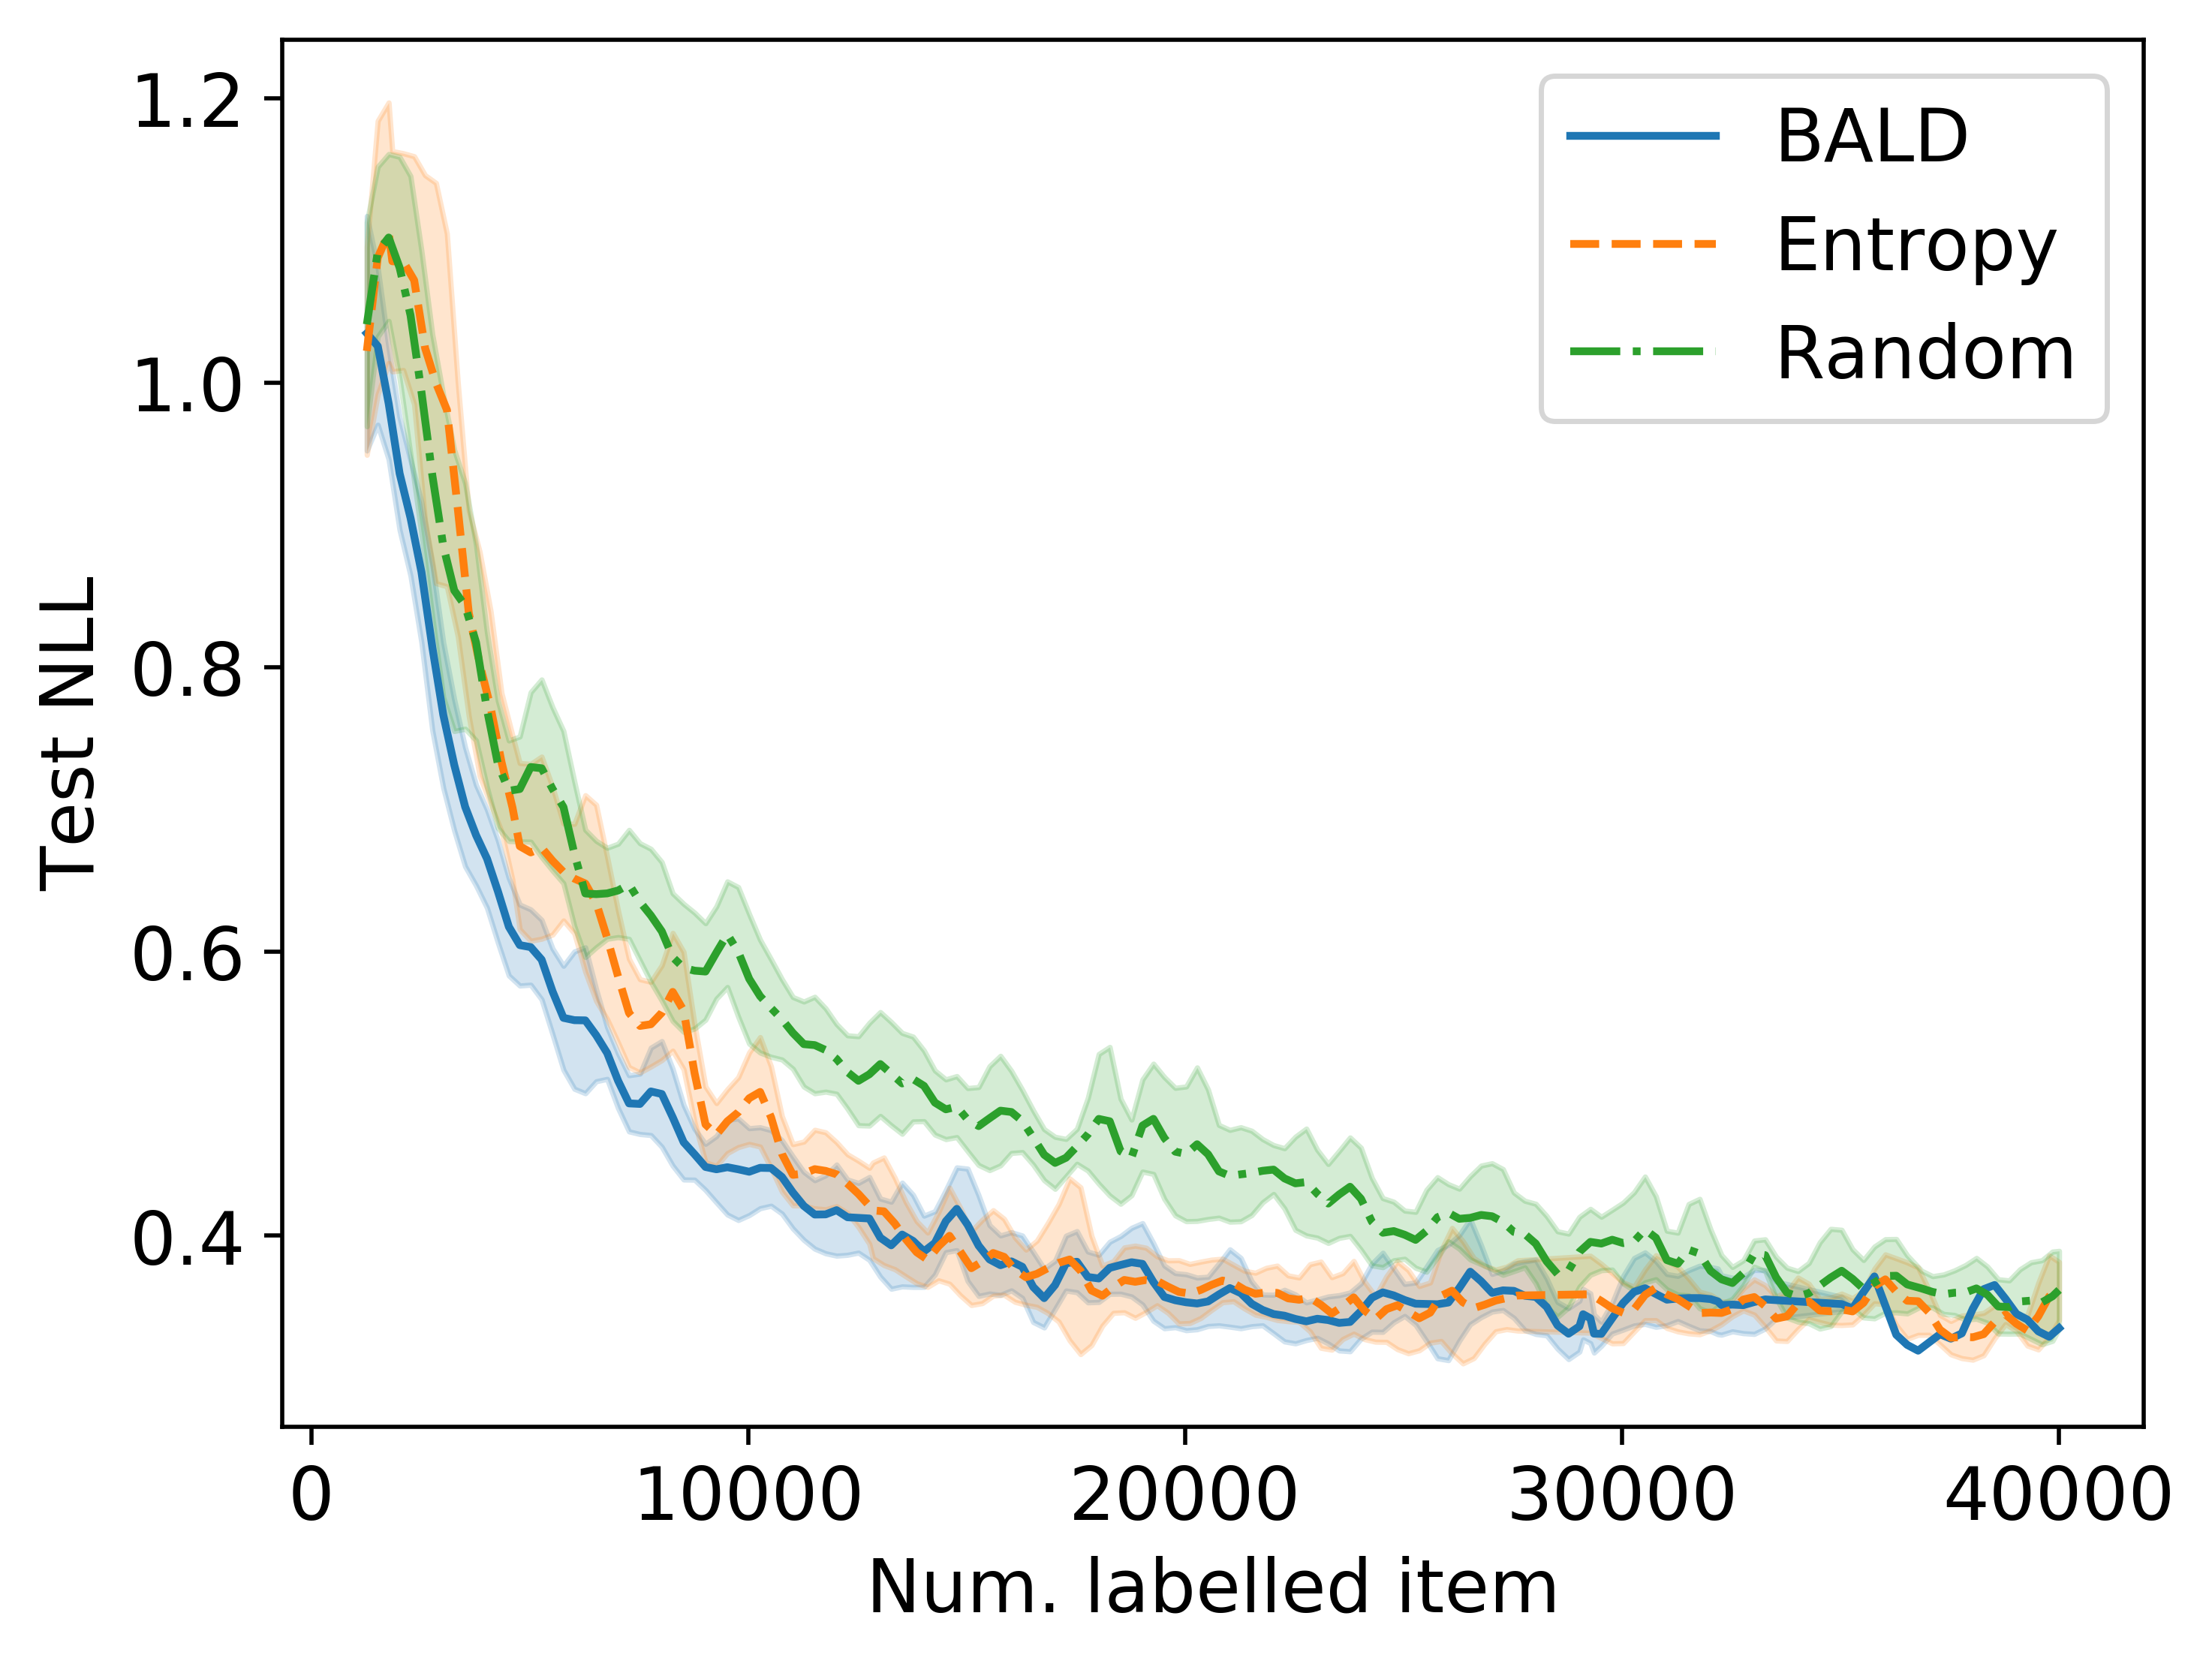
\includegraphics[width=0.4\textwidth]{fig/standard.png}
    \caption{Baselines results on CIFAR10 using MC-Dropout and VGG-16. On an academic dataset, both active learning techniques are competitive.}
    \label{fig:standard}
\end{figure}

\begin{abstract}
\vspace{-0.60cm}
   Active learning is able to reduce the amount of labelling effort by using a machine learning model to query the user for specific inputs.
   While there are many papers on new active learning techniques, these techniques rarely satisfy the constraints of a real-world project. In this paper, we analyse the main drawbacks of current active learning techniques and we present approaches to alleviate them. We do a systematic study on the effects of the most common issues of real-world datasets on the deep active learning process: model convergence, annotation error, and dataset imbalance. We derive two techniques that can speed up the active learning loop such as partial uncertainty sampling and larger query size. Finally, we present our open-source Bayesian active learning library, BaaL.
\end{abstract}

\bibliography{example_paper}
\bibliographystyle{icml2020}
% For submission, needs to be 2 documents and then concat together.
\end{document}



% This document was modified from the file originally made available by
% Pat Langley and Andrea Danyluk for ICML-2K. This version was created
% by Iain Murray in 2018, and modified by Alexandre Bouchard in
% 2019 and 2020. Previous contributors include Dan Roy, Lise Getoor and Tobias
% Scheffer, which was slightly modified from the 2010 version by
% Thorsten Joachims & Johannes Fuernkranz, slightly modified from the
% 2009 version by Kiri Wagstaff and Sam Roweis's 2008 version, which is
% slightly modified from Prasad Tadepalli's 2007 version which is a
% lightly changed version of the previous year's version by Andrew
% Moore, which was in turn edited from those of Kristian Kersting and
% Codrina Lauth. Alex Smola contributed to the algorithmic style files.

%%%%%%%% ICML 2020 EXAMPLE LATEX SUBMISSION FILE %%%%%%%%%%%%%%%%%

\documentclass{article}
\usepackage{times}
\usepackage{epsfig}
\usepackage{graphicx}
\usepackage{amsmath}
\usepackage{amssymb}
\usepackage{times}
\usepackage{epsfig}
\usepackage{graphicx}
\usepackage{amsmath}
\usepackage{amssymb}
% Include other packages here, before hyperref.
\usepackage{xcolor}
\usepackage[ruled,vlined,onelanguage]{algorithm2e}
\usepackage{setspace}
\usepackage{collcell}
\usepackage{xr}
\usepackage{natbib}
\usepackage{multirow}
\usepackage{subcaption}
\usepackage{mathtools}
\usepackage{colortbl,dcolumn}
\usepackage{algorithm2e}

% Include other packages here, before hyperref.

% If you comment hyperref and then uncomment it, you should delete
% egpaper.aux before re-running latex.  (Or just hit 'q' on the first latex
% run, let it finish, and you should be clear).
\usepackage[pagebackref=true,breaklinks=true,letterpaper=true,colorlinks,bookmarks=false]{hyperref}

% \cvprfinalcopy % *** Uncomment this line for the final submission

\def\cvprPaperID{****} % *** Enter the CVPR Paper ID here
\def\httilde{\mbox{\tt\raisebox{-.5ex}{\symbol{126}}}}

\newcommand{\todo}[1]{{\color{blue}TODO #1}}
\newcommand{\toref}[1]{{\color{red}REF #1 }}
\newcommand{\registered}{\textsuperscript{\tiny\textregistered}}
%\newcommand{\etal}{\textit{et al.}}
\renewcommand{\eqref}[1]{\hyperref[#1]{Eq.\ \ref*{#1}}}
\newcommand{\figref}[1]{\hyperref[#1]{Fig.\ \ref*{#1}}}
\newcommand{\tabref}[1]{\hyperref[#1]{Table\ \ref*{#1}}}
\newcommand{\secref}[1]{\hyperref[#1]{Section\ \ref*{#1}}}
\newcommand{\algoref}[1]{\hyperref[#1]{Algorithm\ \ref*{#1}}}
\newcolumntype{C}[1]{>{\centering}m{#1}}
\newcommand{\N}{{\cal N}}
\newcommand{\std}[1]{ \normalfont \color{darkgray}\footnotesize{$\pm$#1} }

% SYMBOL
\newcommand{\E}{{\mathbb E}}

\hypersetup{
    colorlinks=true,
    linkcolor=blue,
    filecolor=magenta,      
    urlcolor=blue,
}

\urlstyle{same}

% Recommended, but optional, packages for figures and better typesetting:
\usepackage{microtype}
\usepackage{booktabs} % for professional tables

% hyperref makes hyperlinks in the resulting PDF.
% If your build breaks (sometimes temporarily if a hyperlink spans a page)
% please comment out the following usepackage line and replace
% \usepackage{icml2020} with \usepackage[nohyperref]{icml2020} above.
\usepackage{hyperref}

% Attempt to make hyperref and algorithmic work together better:
\newcommand{\theHalgorithm}{\arabic{algorithm}}

% Use the following line for the initial blind version submitted for review:
%\usepackage{icml2020}

% If accepted, instead use the following line for the camera-ready submission:
\usepackage[accepted]{icml2020}

% The \icmltitle you define below is probably too long as a header.
% Therefore, a short form for the running title is supplied here:
\icmltitlerunning{Bayesian active learning for production. Supplementary Material}

\begin{document}

\twocolumn[
\icmltitle{Supplementary Material}]

\section{Implementation details}
Our methodology is as follows. We train a VGG-16 \citep{zhang2015accelerating} pretrained on ImageNet~\citep{imagenet_cvpr09}. Our initial training set contains 500 samples. We estimate the uncertainty using 20 MC samples and label the 100 most uncertain elements. Following \citet{gal2017deep}, we reset the weights to their initial value between steps. 

\section{Imbalanced datasets}
 
How to deal with imbalanced datasets is an entire area of research \citep{krawczyk2016learning}, but little has been done to deal with it when we are not aware of the \textit{a priori} class distribution. In consequence, the active learning model may quickly overfit to the more popular classes and reduce the effectiveness of active learning procedure. From \citet{gal2017deep}, it is known that Bayesian active learning will favor underrepresented classes. But, we find the reported experiments to be too simple. We  test this hypothesis in a controlled environment where we can set the number of unrepresented classes. 

In \tabref{fig:imbalanced}, we took the standard CIFAR100 dataset and we mimic an imbalanced dataset where few classes have a high number of examples. A class selected to be underrepresented sees its number of samples to be reduced by 75\%. When we increase the number of underrepresented classes, the gain of using MC-Dropout versus random sampling becomes more obvious. This is due to regions on the learned manifold associated with underrepresented classes to be highly uncertain. In consequence, these regions will be selected for labelling very early in the process.

% In this section, we investigated how common issues in deep learning are affecting active learning. While BALD is robust to data imbalance, it is highly affected by the annotation error or being under fitted.


\begin{table}
    \centering
    \begin{tabular}{llll}
    
    \toprule
    Dataset size &         5000 &        10000 &        20000 \\
    
    \hline
   $\Delta =10$ \\
    BALD &  4.39 \std{0.4} &  3.99 \std{0.01} &  3.57 \std{0.05} \\
    Entropy &  4.71 \std{0.02} &  4.54 \std{0.07} &  3.94 \std{0.01} \\
    Random &  4.52 \std{0.09} &  4.10 \std{0.03} &  3.71 \std{0.05} \\
    \hline
   $\Delta =25$ \\
    BALD &  4.40 \std{0.03}	&4.04\std{0.03} &	3.61\std{0.08} \\
    Entropy &  4.76 \std{0.02} &  4.68 \std{0.08} &   4.00 \std{0.01} \\
    Random &  4.58 \std{0.08} &  4.18 \std{0.04} &  3.75 \std{0.01} \\
    \hline 
   $\Delta =50$ \\
    BALD &  4.49 \std{0.08} &   4.07 \std{0.02} &   3.66 \std{0.04} \\
    Entropy &  4.83 \std{0.04} &  4.60 \std{0.14} &  4.07 \std{0.28} \\
    Random &  4.62 \std{0.03} &   4.21 \std{0.02} &   3.76 \std{0.04} \\
    \end{tabular}
    \caption{Effect of using active learning on imbalanced versions of CIFAR100. $\Delta$ is the number of class that contains 25\% of their data. From \citep{gal2017deep}, we know that BALD is robust to imbalanced datasets, but the study was not extensive. While BALD is robust to imbalanced datasets, the effect is catastrophic when using Entropy.  Performance averaged over 5 runs.}
    \label{fig:imbalanced}
\end{table}

\section{Effect of convergence}

In \figref{fig:active_gain}, we computed the difference in performance between BALD and random. We call this measure the \textit{Active gain} $= NLL_{Random} - NLL_{BALD}$. When using an underfitted model, the gain goes negative i.e. you would be better to use random selection.

\begin{figure}
    \centering
    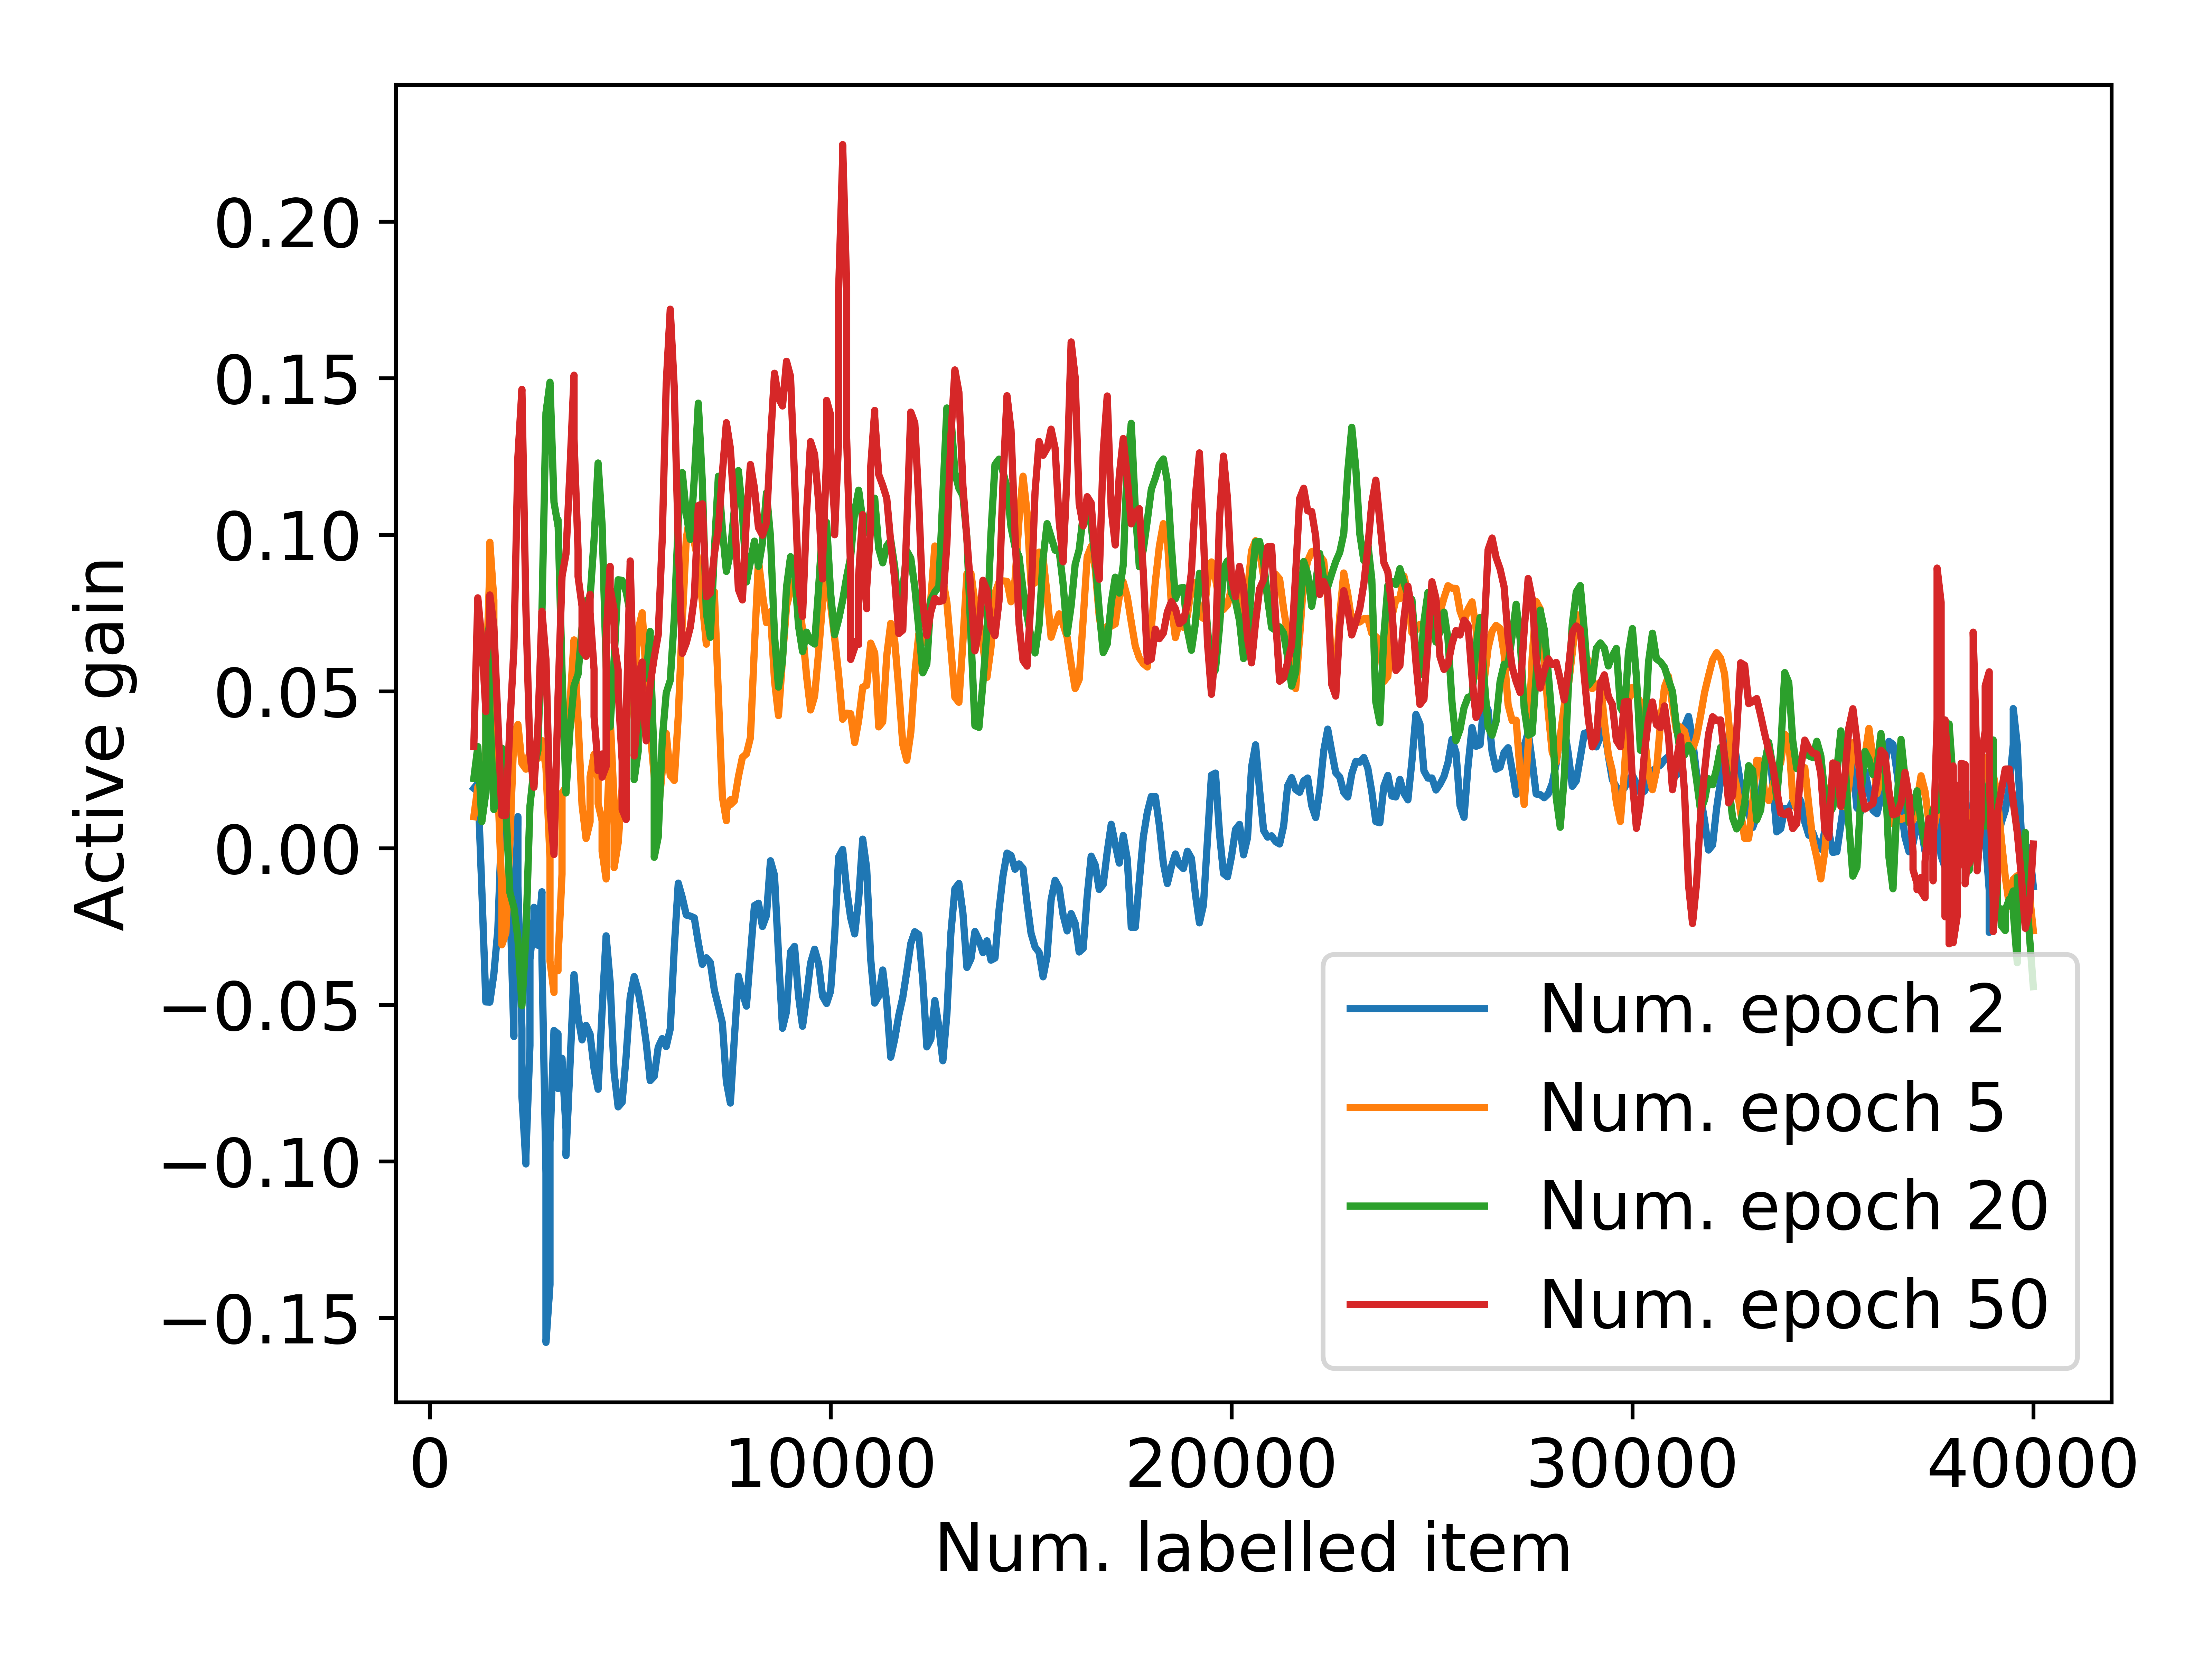
\includegraphics[width=0.5\textwidth]{fig/active_gain.png}
    \caption{Gain of using active learning when varying the number of training epochs. An underfitted model will cause harm to the model training and in this case, just using random would've been better.}
    \label{fig:active_gain}
\end{figure}

\section{Effect of reducing the pool size}
As part of the experiments, we test whether limiting the pool size would affect the performance of active learning. Our experiments in  \figref{fig:pool_size} show that whether to calculate the uncertainty for the whole pool data or a randomly selected subset, the performance of active learning is not affected. This leads to an the interesting outcome of limiting the uncertainty calculations (which is the most expensive part of an active learning loop) in production setup for faster active learning loops.

\begin{figure}
    \centering
    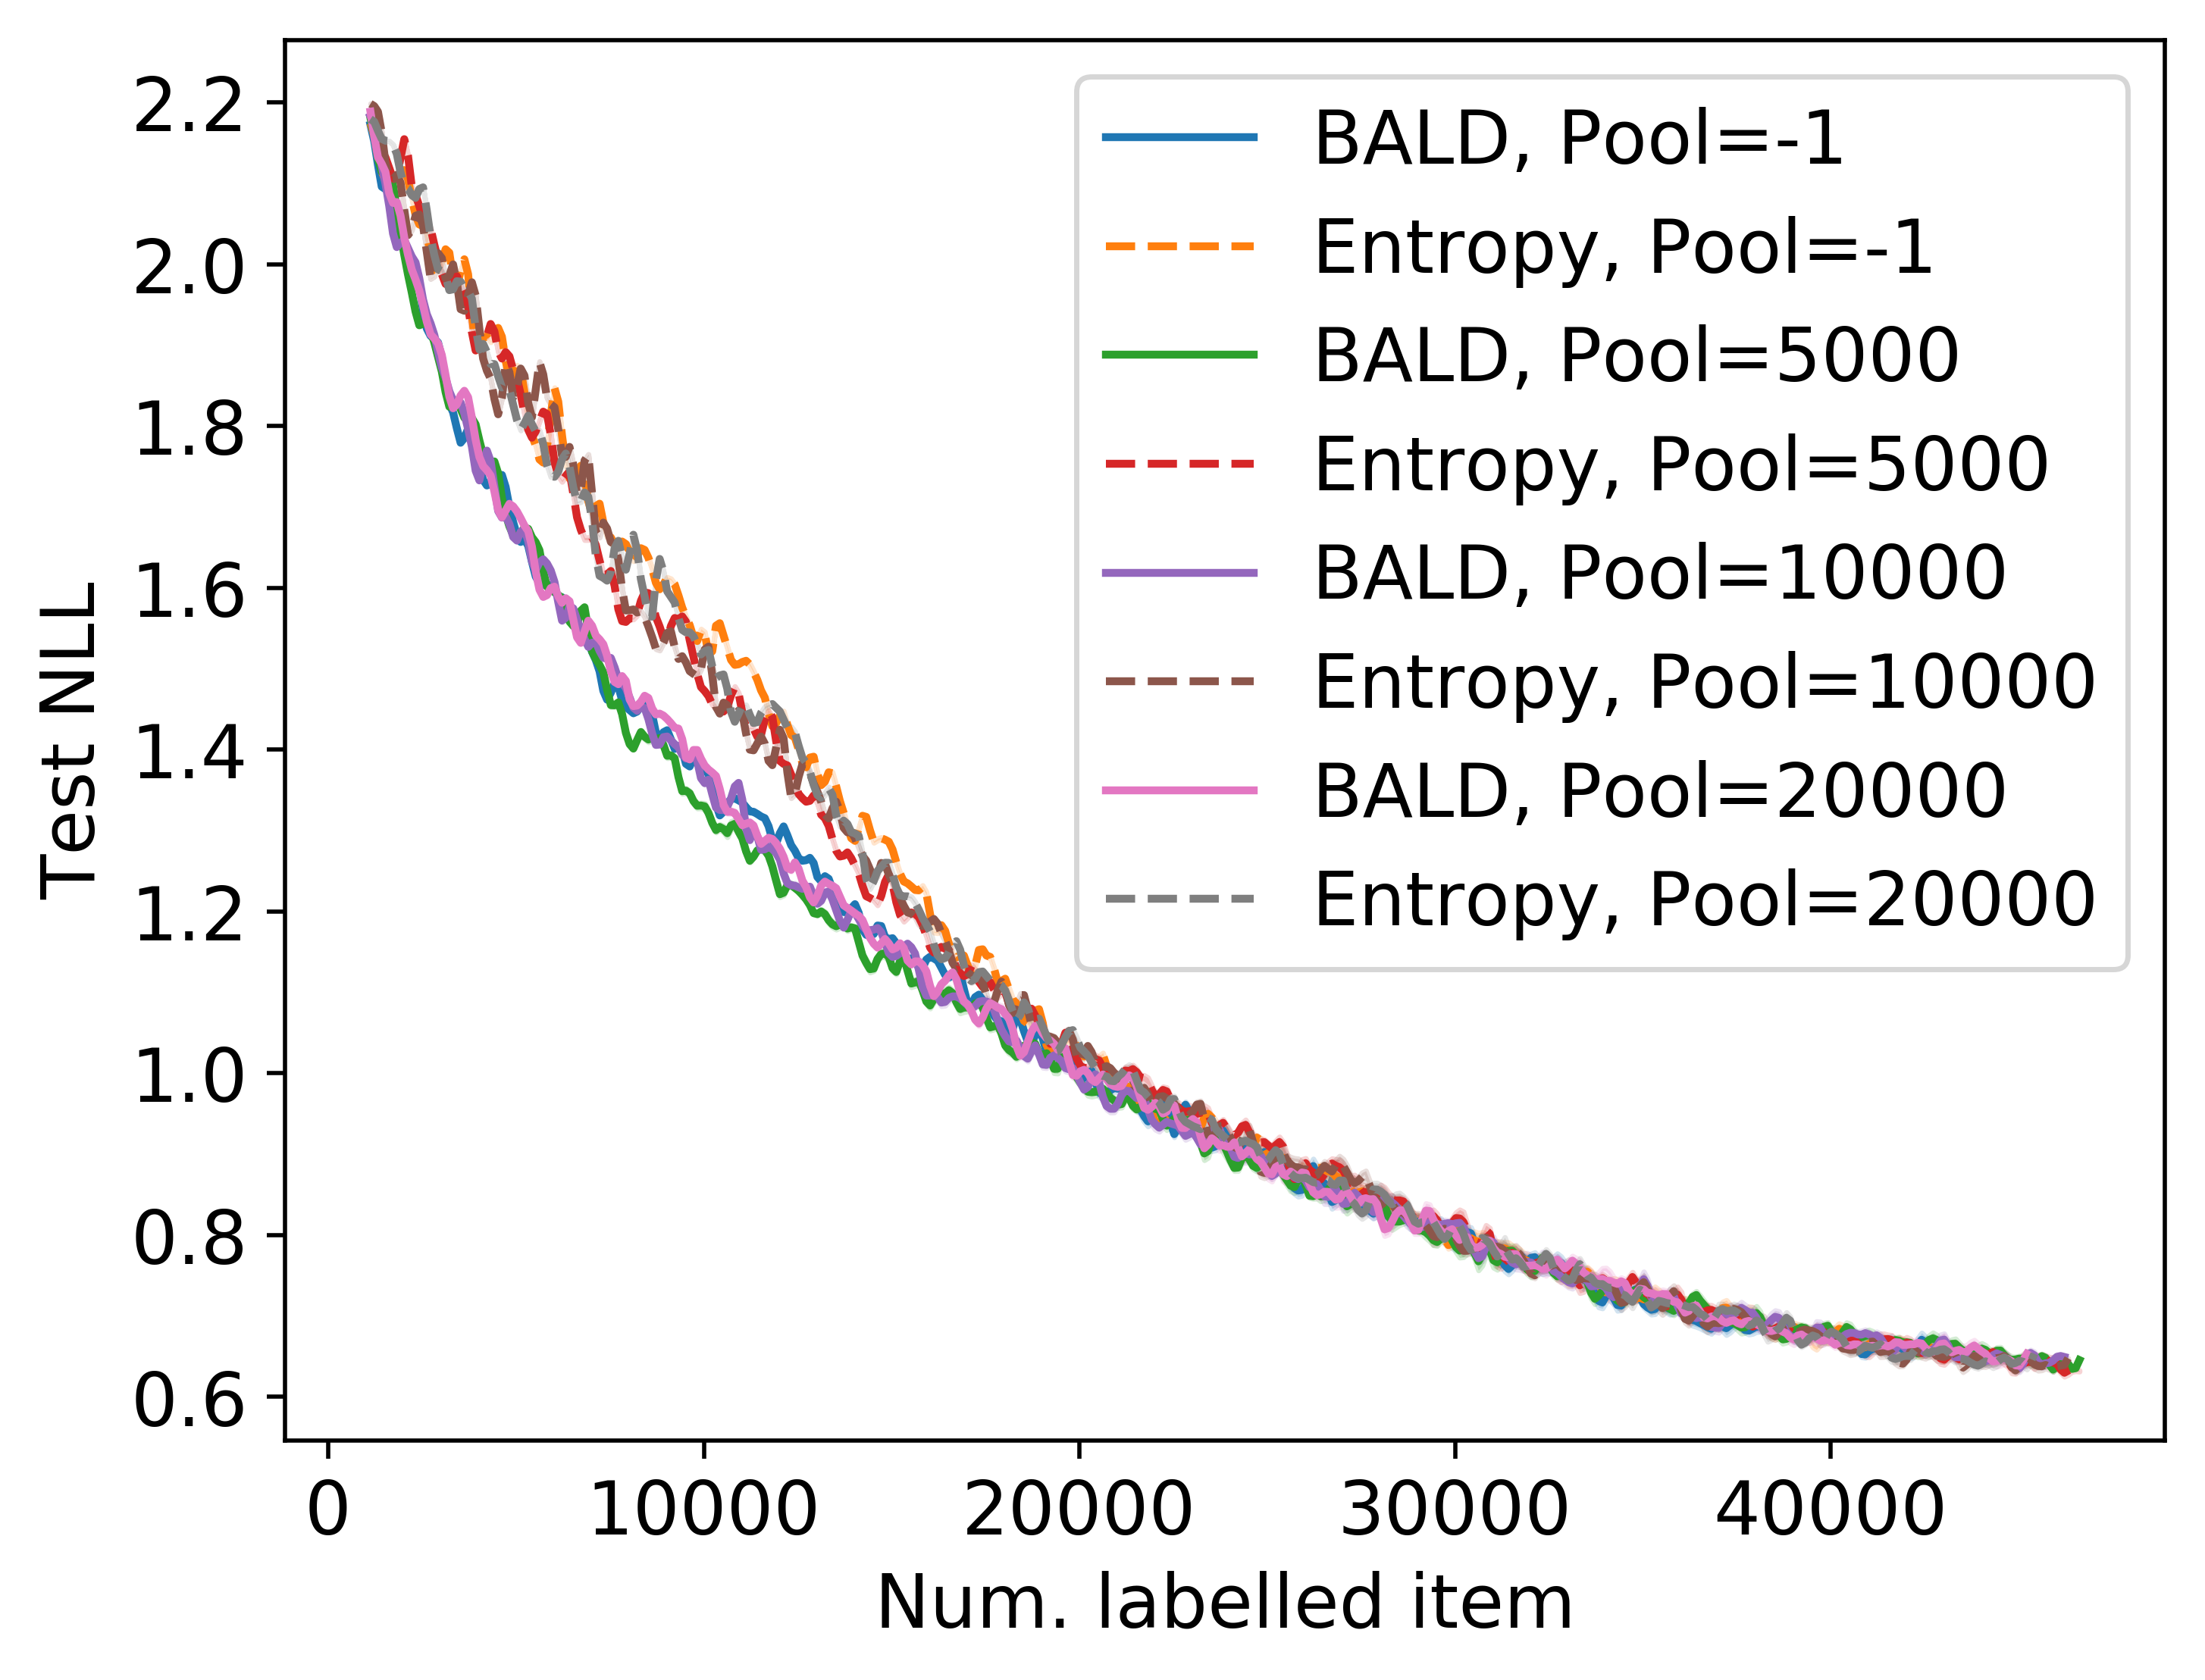
\includegraphics[width=0.4\textwidth]{fig/pol_size.png}
    \caption{Effect of reducing the size of the pool on CIFAR100. \textbf{-1} indicates no reduction. For all heuristics, the performance is not affected by the size of the pool showing that AL can be efficient when tuned properly.  Performance averaged over 5 runs.}
    \label{fig:pool_size}
\end{figure}

\begin{figure}
    \centering
    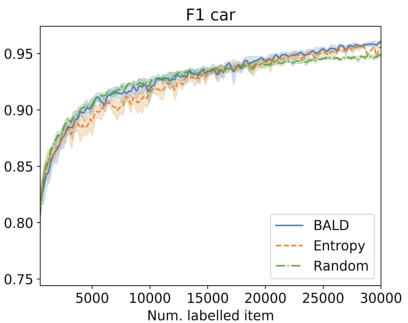
\includegraphics{fig/F1_Mio_tcd_annex.pdf}
    \caption{\textbf{F1 for the class \textit{car}}. BALD is great for underrepresented classes while not affecting more popular classes. Entropy decreases the performance on this class.}
    \label{fig:miotcd}
\end{figure}


\section{Bayesian active learning Library (BaaL)}

All the experiments in this paper have done using our publicly available Bayesian active learning library.  The goal of this library is to provide an easy to use but complete setup to test active learning on any project with few lines of code. We included features that current active learning libraries do not support. In particular, Bayesian methods such as MC-Dropout or Coresets are not widely available and there is no standard implementation of the active learning loop. Furthermore, research codebases are often hard to read and hard to maintain. Our proposed unified API could satisfy both research and industrial users.

 Our recently published open-source package named BaaL, aims at accelerating the transition from research to production. The core philosophy behind our library is to provide researchers with a well-designed API so that they focus on their novel idea and not on technical details. Our library proposes a task-agnostic system where one can mix-and-match any set of acquisition functions and uncertainty estimation methods.
The library consists of three main components:
\begin{enumerate}
    \item Dataset management to keep track and manage the labelled data $D_L$ and the unlabelled data $D_U$.
    \item Bayesian Methods i.e. MC-Dropout, MC-DropConnect and so on.
    \item Acquisition functions i.e. BALD, BatchBALD, Entropy and more.
\end{enumerate}

We provide full support for Pytorch \cite{paszke2017automatic} deep learning modules but our acquisition functions which are the most important part of active learning is implemented in  Numpy\cite{oliphant2006guide} and hence can be used on any platform. Our Data management module keeps track of what is labelled and what is unlabelled. We also provide facilitator methods to label a data point, update the pool of unlabelled data, and to randomly label a portion of the dataset. In our Bayesian module, we provide utilities to make any Pytorch model Bayesian with a single instruction. We also provide training, testing, and active learning loops that facilitate the active training procedure. Our acquisition functions are up-to-date with state-of-the-art methods. We provide easy to follow tutorials (https://baal.readthedocs.io/en/latest/) for each section of the library so that the user understands how each component works. Finally, our library is a member of Pytorch Ecosystem, which is reserved for libraries with outstanding documentation.

Our road-map has been indicated in the repository. Our current focus will include model calibration and semi-supervised learning. As more researchers contribute their methods to our library, we aim to become the standard Bayesian active learning library.

\end{document}
